% ------------------------------------------------------------------------------
% Este fichero es parte de la plantilla LaTeX para la realización de Proyectos
% Final de Grado, protegido bajo los términos de la licencia GFDL.
% Para más información, la licencia completa viene incluida en el
% fichero fdl-1.3.tex

% Copyright (C) 2012 SPI-FM. Universidad de Cádiz
% ------------------------------------------------------------------------------

\documentclass[a4paper,11pt]{book}

% PAQUETES
\usepackage{./estilo/paquetes}
\usepackage{./estilo/colores}
\usepackage{./estilo/comandos}


%Para la indentación al principio de cada párrafo
\setlength{\parindent}{20pt}
\setlength{\parskip}{\baselineskip}

% Ruta al directorio de imágenes
\graphicspath{{./img/}} 

% METADATOS
\title{APERTURA DE DATOS EN APLICACIONES DJANGO}
\author{Iván Ruíz Rube y Juan Manuel Dodero Beardo}
\date{Noviembre 2012}

% Estilo de las citas en latex
\hypersetup{
    citecolor=blue,        % color of links to bibliography
}

\begin{document}

%Para añadir la bibliografía sin necesidad de ser citada
\nocite{*}

%Si ponemos esto, elimina los numeros de pagina y todos los estilos
%\pagestyle{empty}

% PORTADAS
% ------------------------------------------------------------------------------
% Este fichero es parte de la plantilla LaTeX para la realización de Proyectos
% Final de Grado, protegido bajo los términos de la licencia GFDL.
% Para más información, la licencia completa viene incluida en el
% fichero fdl-1.3.tex

% Copyright (C) 2012 SPI-FM. Universidad de Cádiz
% ------------------------------------------------------------------------------


\begin{titlepage}

  \begin{center}

    
\includegraphics[width=0.3\textwidth]{logo-uca.png} \\
    
    \vspace{2.5cm}
    
    \LARGE{\textbf{ESCUELA SUPERIOR DE INGENIERÍA}} \\
    
    \vspace{1.0cm}
    
    \Large{\textbf{INGENIERÍA INFORMÁTICA}} \\
    
    \vspace{3.0cm}
    
    \Large{APERTURA DE DATOS EN PROYECTOS DJANGO} \\
    
    \vspace{2.5cm}
    
    \Large{José Manuel Llerena Carmona} \\
  
    \vspace{0.5cm}

    \large{diciembre de 2013}
    
  \end{center}
\end{titlepage}

\cleardoublepage

% ------------------------------------------------------------------------------
% Este fichero es parte de la plantilla LaTeX para la realización de Proyectos
% Final de Grado, protegido bajo los términos de la licencia GFDL.
% Para más información, la licencia completa viene incluida en el
% fichero fdl-1.3.tex

% Copyright (C) 2012 SPI-FM. Universidad de Cádiz
% ------------------------------------------------------------------------------


\begin{center}

  
\includegraphics[width=0.3\textwidth]{logo-uca.png} \\

  \vspace{2.5cm}

  \Large{ESCUELA SUPERIOR DE INGENIERÍA} \\

  \vspace{1.0cm}

  \large{INGENIERÍA EN INFORMÁTICA} \\

  \vspace{2.0cm}

  \large{APERTURA DE DATOS EN PROYECTOS DJANGO} \\

  \vspace{2.5cm}

\end{center}

\begin{itemize}
\item \large{Departamento: Ingeniería Informática}
\item \large{Directores del proyecto: Iván Ruíz Rube y Juan Manuel Dodero Beardo}
\item \large{Autor del proyecto: José Manuel Llerena Carmona}
\end{itemize}

\vspace{0.2cm}

\begin{flushright}
  \large{Cádiz, diciembre de 2013} \\

  \vspace{2.5cm}
  \begin{tabular}{ccc}
  \large{Fdo: Iván Ruíz Rube} & \large{Fdo: Juan M. Dodero Beardo} & \large{Fdo: José M. Llerena Carmona}\\
  \end{tabular}
\end{flushright}

\cleardoublepage

% PRELIMINARES
% ------------------------------------------------------------------------------
% Este fichero es parte de la plantilla LaTeX para la realización de Proyectos
% Final de Grado, protegido bajo los términos de la licencia GFDL.
% Para más información, la licencia completa viene incluida en el
% fichero fdl-1.3.tex

% Copyright (C) 2012 SPI-FM. Universidad de Cádiz
% ------------------------------------------------------------------------------

\thispagestyle{empty}

\noindent \textbf{\begin{Large}\textit{Agradecimientos}\end{Large}} 
\newline
\newline
\noindent\textit{A mis padres, por haberme dado la oportunidad de estudiar, ya
que sin ellos nunca lo podría haber conseguido.}

\noindent\textit{A mi novia Isabel, por haber estado siempre a mi lado
apoyándome.}

\noindent\textit{A mis tutores Don Iván Ruíz Rube y Don Juan Manuel Dodero
Beardo, a los que les agradezco sinceramente toda la ayuda y consejos que me han
prestado.}

\newpage

% ------------------------------------------------------------------------------
% Este fichero es parte de la plantilla LaTeX para la realización de Proyectos
% Final de Grado, protegido bajo los términos de la licencia GFDL.
% Para más información, la licencia completa viene incluida en el
% fichero fdl-1.3.tex

% Copyright (C) 2012 SPI-FM. Universidad de Cádiz
% ------------------------------------------------------------------------------

\thispagestyle{empty}

\noindent \textbf{\begin{Large}Resumen\end{Large}} 
\newline
\newline
\noindent Hoy en día es mucha la información que circula a través de internet, y
aunque la gran mayoría sea comprensible por el ser humano, las máquinas no
disponen de la capacidad de razonamiento necesario para comprender en muchos de
los casos de qué trata dicha información o con qué está relacionada. De esta
forma, mediante el marcado de nuestros datos haciendo uso de vocabularios
específicos, podemos dotar a nuestro contenido web de un mayor valor semántico
(web semántica), de tal forma que estemos indicando explícitamente qué es la
información que estamos publicando.

\noindent En el presente proyecto titulado Apertura de datos en aplicaciones
Django, se ha desarrollado una herramienta para el framework de desarrollo web
Django, el cual se encuentra desarrollado bajo el lenguaje de programación
Python. Esta herramienta o plugin, se encargará de facilitar al usuario la
publicación controlada de los datos de sus proyectos Django en internet,
haciendo uso de los vocabularios u ontologías disponibles en internet para tal
finalidad.

\noindent En la web están disponibles multitud de ontologías disponibles para
los usuarios que deseen hacer uso de ellas. Cada una de ellas relacionadas con
una temática diferente o con muchas temáticas a la vez, como por ejemplo puede
ser, la música, la ingeniería, el cine, electrónica, etc\ldots

\noindent A día de hoy, multitud de organizaciones, tanto públicas como privadas,
usuarios y software están adaptando sus productos a la web semántica para la
apertura de sus datos. Un ejemplo bastante claro es el Open Government (o
gobierno abierto), donde se defiende que los temas del Gobierno y
Administración Pública se abran a los ciudadanos, de tal forma que se transmita
transparencia en sus gestiones. También en el ámbito del comercio, aplicaciones
bastante populares de comercio electrónico, están adaptando o han adaptado sus
aplicaciones para la publicación de sus datos, confiriendo de esta forma una
mayor proyección de los productos.

\noindent A raíz de todo esto comentado, surge la idea de realizar una
herramienta para un framework de desarrollo web cada vez más usado, que permita
adaptar los proyectos existentes a la publicación de datos, sin necesidad de
redesarrollar los proyectos por completo.

\noindent Por lo tanto, la herramienta que se ha desarrollado en el presente
proyecto, permitirá a partir de sus datos realizar un etiquetado de los mismos
para luego publicar estos en internet. Para desarrollar esto, la presente
herramienta ofrece al usuario las siguientes funcionalidades:
\begin{itemize}
    \item Captación de los datos de los que está compuesto nuestro proyecto
        Django.
    \item Carga de espacios de nombres y ontologías definidas en la web que
        sirvan para el propósito de los datos que se desean publicar.
    \item Posibilidad de elegir qué datos van a ser publicados y cuales no lo
        serán.
    \item Componente para la interrelación de los espacios de nombres y los datos de nuestro proyecto.
    \item Componente para la publicación de nuestros datos en diferentes
        formatos existentes.
\end{itemize}

\noindent {\bf Palabras clave:} OpenData, LinkedData, RDF, RDFa, Microdata,
ontología, namespace, \mbox{RDF/Ntriples}, RDF/Turtle, XML, Django, Python, SPARQL,
D2Rq.

\newpage


\frontmatter

% INDICES
\tableofcontents
\listoffigures
\listoftables

\mainmatter

% PROLEGÓMENO
\part{Prolegómeno}
%\null\vfill
%\noindent La primera parte de la memoria del PFC debe contener una introducción y una planificación del proyecto.\\

%La introducción es un capítulo que, a modo de resumen, debe contener una breve descripción del contexto de la disciplina en la que el proyecto tiene aplicación, la motivación para su desarrollo, una explicación de la situación actual previa al proyecto y de otros sistemas existentes, en su caso, y la problemática existente que se pretende solucionar. Al final del capítulo introductorio se deben enunciar claramente los objetivos y el alcance del proyecto.\\

%El segundo capítulo debe incluir una planificación del proyecto. La planificación deberá ajustarse a las prácticas de ingeniería en general, y de la ingeniería del software en particular. Deberá tener en cuenta los plazos, los entregables (documentos y software), los recursos (humanos y de equipamiento inventariable) y el método de ingeniería de software a emplear.
%\\

\chapter{Introducción}
% ------------------------------------------------------------------------------
% Este fichero es parte de la plantilla LaTeX para la realización de Proyectos
% Final de Grado, protegido bajo los términos de la licencia GFDL.
% Para más información, la licencia completa viene incluida en el
% fichero fdl-1.3.tex

% Copyright (C) 2012 SPI-FM. Universidad de Cádiz
% ------------------------------------------------------------------------------

A lo largo del siguiente documento, se describirán las motivaciones que han
llevado a la realización del proyecto, así como los objetivos, estructura,
requisitos y demás características técnicas, implementación y pruebas del mismo,
además de los manuales necesarios para su utilización.

Como punto inicial, en el presente capitulo se describen la motivaciones para la
realización del proyecto, los objetivos y cómo se encuentra estructurada la
documentación.

\section{Motivación}

Actualmente existe una gran cantidad de datos distribuidos por toda la red, pero
éstos no se encuentran publicados ni organizados de forma que otros usuarios u
organizaciones puedan hacer uso de ellos, o mejor dicho, de forma que otras
aplicaciones externas puedan entenderlos. Especificando un formato común para
publicar dicha información, se podrían obtener grandes cantidades de información
en la web, a disposición de cualquier usuario u organización que la desease.

Hoy en día muchos Gobiernos (OpenGovernment) están abriendo parte de sus datos
en la Web, beneficiando así a multitud de usuarios, los cuales pueden captar
estos datos y generar estadísticas, informes, estudios, generando transparencia
en la gestión del gobierno. O como en el caso del comercio electrónico, si un
comerciante abre sus datos en la Web, los buscadores pondrán enlazar mucho mejor
sus productos, y ofrecer mejores resultados de búsqueda para su Web de comercio
electrónico. Como conclusión, podemos decir que la apertura de datos, es
beneficiosa en multitud de casos totalmente distintos, tanto como el marketing,
investigación, gobierno, etc\ldots

A raíz de todo esto, surgen multitud de vocabularios (ontologías) donde se
definen una serie de entidades y propiedades de las mismas, con las cuales
podemos relacionar nuestros datos. También existen multitud de estándares los
cuales nos permiten realizar la publicación de los datos en un formato conocido.
Por lo que, cuando vayamos a abrir nuestros datos podremos darle una estructura
conocida por todos, de forma que aquella persona que vaya a hacer uso de ellos,
pueda conocer a qué hacen referencia los mismos. De esta forma, conseguimos
darle un significado semántico a los datos que estamos mostrando en nuestra web.
Además, podremos definir relaciones entre los distintos datos, tanto los
pertenecientes a nuestros proyectos como de otras fuentes externas, lo cual se
conoce como LinkedData.

\section{Descripción del sistema actual}

En la actualidad, para el framework de desarrollo de aplicaciones web Django, no
existen aplicaciones (o éstas ofrecen pocas funcionalidades o se encuentran
obsoletas) que permitan realizar la apertura de datos de proyectos Django a
través de un menú de configuración intuitivo, haciendo uso de cualquiera de las
diferentes ontologías disponibles en internet para el marcado de los datos, como
pueden ser por ejemplo:
\begin{itemize}
    \item \textbf{Schema \cite{schema}:} proporciona un vocabulario para
        marcar los contenidos web, el cual es reconocido por los principales
        buscadores, como son: Google, Bing, Yahoo o Yandex.
    \item \textbf{FOAF \cite{foaf}:} acrónimo de Friend Of A Friend, define
        una ontología para la publicación de relaciones entre personas y datos
        en internet.
    \item \textbf{Good relations \cite{GoodRelations}:} similar a los
        anteriores, define un vocabulario específico para el comercio
        electrónico. Dicho vocabulario, ya ha sido incluido en la especificación
        de Schema.
\end{itemize}

Por otro lado, actualmente si que existen herramientas de este tipo realizadas
para otros frameworks de desarrollo de aplicaciones Web, como puede ser el caso
de una gema realizada para el framework Ruby on Rails, bajo el nombre de
EasyData\footnote{El proyecto se encuentra alojado en el repositorio
\url{https://github.com/jnillo/Linked_data}}, desarrollada también en la
Universidad de Cádiz, que ha obtenido buenos resultados. Al igual que
también conocidas aplicaciones de comercio electrónico realizadas en PHP, como
puede ser Magento o Prestashop, también están siguiendo esta tendencia y se
están adaptando al espacio de la Web semántica, vista las ventajas que ofrece.
Por lo tanto, a raíz de la utilidad del mismo y que prueba de ello cada vez más
tecnologías se están adaptando, sería interesante disponer de una herramienta de
este tipo, en un framework como Django, que cada vez está más presente en el
total de aplicaciones existentes en la Web.

\section{Objetivos y alcance del proyecto}
\label{sec:objetivos}

El objetivo principal del presente proyecto es el de proporcionar al
desarrollador de aplicaciones Django, una herramienta (conocida a partir de
ahora como EasyData/Django) la cual le permita realizar la apertura
\textbf{controlada} de los datos de su proyecto Django. Esto es el producto
final que se obtendrá al finalizar dicho proyecto, pero este proyecto se puede
desgranar en objetivos más específicos o subobjetivos, donde la unión de estos
formen la totalidad del proyecto. Estos objetivos más específicos, se pueden
dividir en tres, los cuales son:


%%%TABLA - Objetivo 001
\begin{center}
\begin{longtable}{||p{3.4cm}|p{12cm}||}
%primera parte de la tabla
 \hline \hline \bf OBJ-001 &  \bf Resolver modelos de la aplicación \\
\hline
\endfirsthead
%primera parte de la tabla por pagina
\hline \multicolumn{2}{|r|}{{Continuación de la tabla}} \\ \hline
 \hline \bf OBJ-001 &  \bf Resolver modelos de la aplicación \\
\hline
\endhead
% ultima parte de la tabla por pagina
\hline \multicolumn{2}{|l|}{{Continúa en la siguiente página}} \\ \hline
\endfoot
% ultima parte de la tabla
\endlastfoot
% DATOS
 \hline \bf Autor & José Manuel Llerena Carmona \\
 \hline \bf Descripción & Un primer objetivo será realizar una parte software,
             que sea capaz mediante introspección, de obtener los distintos
             modelos, junto con los fields y relaciones y los tipos de estos dos
             últimos que componen el proyecto Django donde se encuentra
             instalado nuestro proyecto. Esta estructura se almacenará, para
             posteriormente poder realizar la configuración de cómo se va a
             llevar a cabo la publicación de los datos.\\
 \hline \bf Subobjetivos & 
             \begin{itemize}
                 \item Confeccionar una estructura de base de datos, que
                        permita almacenar la estructura de modelos que forman el
                        proyecto Django donde se encuentra nuestra aplicación.
                 \item Desarrollar una porción de software, la cual sea capaz de
                        obtener la estructura de los modelos del proyecto Django
                        donde nos encontramos, y almacenar esta estructura en la
                        base de datos confeccionada anteriormente.
             \end{itemize}\\
\hline
\hline
\caption{\label{tab:obj001} Objetivo - 001 - Resolver modelos de la aplicación} 
\end{longtable}
\end{center}


%%%TABLA - Objetivo 002
\begin{center}
\begin{longtable}{||p{3.4cm}|p{12cm}||}
%primera parte de la tabla
 \hline \hline \bf OBJ-002 &  \bf Interfaz de configuración \\
\hline
\endfirsthead
%primera parte de la tabla por pagina
\hline \multicolumn{2}{|r|}{{Continuación de la tabla}} \\ \hline
 \hline \bf OBJ-002 &  \bf Interfaz de configuración \\
\hline
\endhead
% ultima parte de la tabla por pagina
\hline \multicolumn{2}{|l|}{{Continúa en la siguiente página}} \\ \hline
\endfoot
% ultima parte de la tabla
\endlastfoot
% DATOS
 \hline \bf Autor & José Manuel Llerena Carmona \\
 \hline \bf Descripción & Un segundo objetivo consistirá en proporcionar al
             usuario una aplicación Web de configuración, donde podrá detallar
             cómo se va a realizar la apertura de datos de su proyecto. En este
             apartado, el usuario deberá de indicar con qué entidades de los
             vocabularios disponibles en la aplicación, se relacionan los
             modelos de su proyecto, y con qué propiedades de dichas entidades,
             se relacionan los atributos y relaciones de cada uno de los modelos.
             Además se podrá especificar para cada uno de los modelos, cuales
             serán visibles y cuales no (no todos los datos son susceptibles de
             ser publicados, ya que todo proyecto puede contener datos sensibles
             o que se encuentren protegidos por leyes de protección de datos).\\
 \hline \bf Subobjetivos &
             \begin{itemize}
                 \item Proporcionar un apartado dentro del proyecto, donde el
                        usuario sea capaz de cargar los diferentes vocabularios
                        u ontologías que va a utilizar para la publicación de
                        los datos.
                 \item Proporcionar un apartado donde se listen los distintos
                        modelos que componen al proyecto Django, de tal forma
                        que para cada uno de los modelos, pudiésemos especificar
                        con qué entidades de las propuestas por las distintas
                        organizaciones se corresponden.
                 \item Un apartado más dónde para cada modelo, se pudiera
                        realizar la correspondencia (mapeo) de cada uno de los
                        fields del modelo con las propiedades de la entidad
                        asociada al modelo o cualquier otra disponible en el
                        namespace.
                 \item Un último apartado, donde para cada modelo y field o
                        relación de nuestros modelos, podamos indicar si estos
                        son visibles o no.
             \end{itemize}\\
\hline
\hline
\caption{\label{tab:obj002} Objetivo - 002 - Interfaz de configuración} 
\end{longtable}
\end{center}


%%%TABLA - Objetivo 003
%TODO: si se puede, desgranar también este apartado, cuando sepa mejor las posibles formas de mostrar los datos que se van a emplear.
\begin{center}
\begin{longtable}{||p{3.4cm}|p{12cm}||}
%primera parte de la tabla
 \hline \hline \bf OBJ-003 &  \bf Publicación de datos \\
\hline
\endfirsthead
%primera parte de la tabla por pagina
\hline \multicolumn{2}{|r|}{{Continuación de la tabla}} \\ \hline
 \hline \bf OBJ-003 &  \bf Publicación de datos \\
\hline
\endhead
% ultima parte de la tabla por pagina
\hline \multicolumn{2}{|l|}{{Continúa en la siguiente página}} \\ \hline
\endfoot
% ultima parte de la tabla
\endlastfoot
% DATOS
 \hline \bf Autor & José Manuel Llerena Carmona \\
 \hline \bf Descripción & Un tercer y último objetivo sería el de proporcionar
             al usuario, una serie de herramientas, las cuales le permitan
             realizar la publicación de los datos de su proyecto. Estas le
             permitirían al usuario utilizar los distintos tipos de notaciones
             más comúnmente usados, como pueden ser RDF/XML, RDF/Turtle,
             RDF/Ntriples, Microdata o RDFa.\\
\hline
\hline
\caption{\label{tab:obj003} Objetivo - 003 - Publicación de datos} 
\end{longtable}
\end{center}


Por lo tanto, como conclusión a todo lo comentado, el alcance del proyecto será
el de proporcionar al usuario, una aplicación Django, que le permita realizar la
apertura de los datos de forma controlada de sus proyectos Django en la Web.
Para ello, la aplicación le proporcionará al usuario, la posibilidad de usar la
mayor parte de los formatos permitidos en la Web semántica para la publicación
de datos en internet. Así como también le permitirá la carga de las diferentes
ontologías existentes en la web, de tal forma que la aplicación se adaptará a
cualquier nuevo espacio de nombres que pueda surgir en un futuro.

\newpage

\section{Definiciones}

\begin{description}
    \item[Framework] \hfill \\
        en el ámbito del desarrollo software, se entiende por framework a una
        plataforma software para desarrollar aplicaciones, la cual sirve como
        base para el desarrollo.
    \item[Modelo] \hfill \\
        es uno de los componentes del patron Modelo-Vista-Controlador. El modelo
        se encarga de representar y gestionar toda la información con la que el
        sistema trabaja.
    \item[Vista] \hfill \\
        es otro de los componentes del patron Modelo-Vista-Controlador. En el
        caso de Django, la vista hace referencia al controlador, aunque exista
        otro componente con el nombre de vista. Las vistas en Django se encarga
        de responder a eventos y tratar la información realizando peticiones a
        los modelos. Las vistas pueden utilizar las plantillas, para mostrar los
        datos generados en ellas.
    \item[Plantilla] \hfill \\
        es otro de los componentes del patron Modelo-Vista-Controlador. En el
        caso de Django, la plantilla hace referencia a la vista del patrón MVC.
        La plantilla se encarga de presentar los datos en un formato adecuado
        para la interacción.
    \item[Ontología o Namespace] \hfill \\
        dentro de la aplicación que se va a desarrollar, se conoce por ontología
        o namespace, a cada uno de los vocabularios definidos que están
        disponibles para que los usuarios realicen el marcado del contenido de
        sus datos.
    \item[Python] \hfill \\
        \cite{python} es el lenguaje de programación que se va a utilizar para el desarrollo
        del proyecto. Este lenguaje de programación es multiparadigma, ya que
        permite la utilización de diferentes paradigmas de programación
        (orientado a objetos, funcional o imperativa). Este lenguaje de
        programación también se caracteriza por ser multiplataforma y de código
        abierto. Para más información se puede consultar la web oficial de
        \href{http://es.wikipedia.org/wiki/Python}{Python}.
    \item[Django] \hfill \\
        se trata de un framework de desarrollo web de código abierto, el cual se
        utilizará para la realización del proyecto. Este framework está escrito
        en el lenguaje de programación Python y está basado en el modelo MVC
        (Modelo Vista Controlador).
    \item[RDF] \hfill \\
        \cite{rdfdoc} es el acrónimo de Resource Description Framework. Está diseñado por el
        World Wide Web Consistorium como un modelo de datos para metadatos. Se
        usa para la descripción conceptual y modelado de la información para
        recursos web.
    \item[RDFa] \hfill \\
        es el acrónimo de Resource Description Framework in Attributes. Se trata
        de una serie de extensiones para lenguajes HTML, XHTML y ciertos
        documentos basados en XML recomendadas por W3C, de forma que se permita
        dotar de contenido semático a los documentos web.
    \item[Microdata] \hfill \\
        es una especificación HTML de WHATWG (Web Hypertext Application
        Technology Working Group), para enlazar metadatos al contenido existente
        en páginas web.
    \item[Web semántica] \hfill \\
        es un conjunto de actividades promovidas por el W3C con la finalidad de
        crear tecnologías que permitan la publicación de datos legibles por
        aplicaciones informáticas.
\end{description}

\section{Organización del documento}

Este documento tiene como finalidad, describir todo el proceso de desarrollo de
la aplicación Django para la apertura de datos de proyectos y su posterior
publicación, empezando por la descripción de los objetivos iniciales y
requisitos esenciales que deberá reunir dicho proyecto. Se mostrará una
planificación del desarrollo del proyecto, incluyendo costes estimados y
diagramas de Gantt que ilustren el avance del proyecto en el tiempo.

En este documento también se plasmará todo el ciclo de vida de desarrollo, desde
la fase de análisis y diseño de los requisitos del proyecto, definiendo los
distintos casos de usos, diagramas con la organización de los datos, actores
implicados o diagramas de secuencia e interacción que pudieran resultar del
mismo. Siguiendo por la implementación del mismo y las pruebas realizadas, las
cuales verifiquen la calidad y robustez del mismo. Además, en este documento
también se comentarán las posibles mejoras o ampliaciones futuras que pudieran
considerarse.

Por último, proporcionará al usuario tanto un manual de uso, como un manual de
instalación y explotación del mismo, de tal forma que cualquier usuario sin
conocimientos previos de la aplicación, pueda hacer uso de ella y sacarle el
máximo partido posible.


\chapter{Planificación}
% ------------------------------------------------------------------------------
% Este fichero es parte de la plantilla LaTeX para la realización de Proyectos
% Final de Grado, protegido bajo los términos de la licencia GFDL.
% Para más información, la licencia completa viene incluida en el
% fichero fdl-1.3.tex

% Copyright (C) 2012 SPI-FM. Universidad de Cádiz
% ------------------------------------------------------------------------------


En esta sección se describen todos los aspectos relativos a la planificación del
proyecto: metodología, organización, costes, planificación y gestión de riesgos.

\section{Metodología de desarrollo}

Como metodología de desarrollo para la elaboración del proyecto, nos hemos
basado en el modelo de ciclo de vida de desarrollo en espiral. Este modelo de
desarrollo se centra en dividir el proyecto en segmentos más pequeños y
proporcionar más facilidad de cambio en el proceso de desarrollo. En este
modelo, se combinan las principales características del desarrollo
iterativo, con las del desarrollo en cascada, de forma que en cada uno de las
iteraciones en la espiral, recoge todas fases del modelo en cascada, de
tal forma, que al final de cada iteración, obtenemos una porción de software,
y en las sucesivas iteraciones se obtienen versiones incrementales de la misma
pieza software. Tal y como explicamos en el capítulo anterior, nuestro proyecto
lo hemos dividido en varias piezas software ``independientes'', de tal forma
haciendo uso de este modelo, nos permitirá realizar el desarrollo por partes,
obteniendo en cada una de las iteraciones de la espiral, una de las piezas
software definidas anteriormente.

Para el modelo de ciclo de vida de desarrollo en espiral, se definen cuatro
fases, las cuales son las que se repiten en cada una de las iteraciones de la
espiral. Estas fases son las siguientes:
\begin{itemize}
    \item \textbf{Definición de objetivos:} Exceptuando la planificación inicial,
           que es llevada a cabo al comienzo del proyecto, en esta fase en cada
           una de las iteraciones de la espiral se especifican y analizan los
           requisitos que deberá cumplir el componente software, al final de la
           iteración para cumplir cada uno de los objetivos en los que hemos
           dividido el proyecto.
    \item \textbf{Análisis de riesgos:} En esta fase se evalúan los posibles
           riesgos y eventos no deseados que puedan surgir durante la ejecución
           de la iteración, para que en la fase de desarrollo y pruebas, se
           puedan evaluar los mismos y buscar las alternativas posibles para
           solventarlos.
    \item \textbf{Desarrollo y pruebas:} En este apartado se realizan las
           tareas propias que su nombre indica, se lleva a cabo el diseño e
           implementación de los requisitos especificados, y se prueban los
           mismos. Además, en este apartado, como se acaba de comentar, se
           evalúan las posibles alternativas para solventar los posibles riesgos
           existentes. Al final de esta fase, se obtiene la nueva versión
           incremental del software.
    \item \textbf{Planificación:} En esta fase se revisan el producto obtenido,
           y se decide si se continúa con la siguiente iteración.
\end{itemize}


\section{Planificación del proyecto}
A continuación se va a realizar una estimación temporal del tiempo que se
empleará en la elaboración del proyecto. Para ello, vamos a dividir el proyecto
en una serie de fases, las cuales según la complejidad y extensión de las
mismas, se le asignará un tiempo estimado para su finalización.

\subsection{Especificación de las Fases}

Las fases en las que vamos a dividir nuestro proyecto para realizar la
estimación temporal, son las siguientes:

\begin{itemize}
    \item \textbf{Estudio inicial:} este apartado hace referencia al estudio
           de la propuesta de proyecto, redacción del proyecto y motivaciones
           del mismo. Comprende desde las primeras reuniones con los tutores del
           proyecto donde se propone el mismo, hasta el momento de la asignación
           de este.
    \item \textbf{Preparación del entorno:} esta parte se refiere a todas las
           tareas realizadas para la preparación del entorno de trabajo para
           elaborar el proyecto. Desde la solicitud de apertura de un espacio de
           trabajo y un repositorio SVN para alojar el proyecto, hasta la
           selección e instalación de las herramientas necesarias para realizar
           el mismo, como pueden ser el IDE, el sistema de control de versiones,
           servidores o configuración de la máquina.
    \item \textbf{Fase de Análisis\footnote{\label{pie}Estos apartados se
           repetirán varias veces a lo largo del desarrollo del proyecto, ya que
           al hacer uso de una metodología de desarrollo en espiral, en cada una
           de las iteraciones de la metodología, tendremos que volver a revisar
           cada uno de los requisitos, para determinar si se cumplen o si estos
           se adaptan a los requisitos verdaderos de la aplicación, y continuar
           con la implementación y/o corrección de los requisitos existentes y
           realizar las pruebas de los mismos.}:} el apartado de fase de
           análisis, se corresponde totalmente con la fase de análisis del ciclo
           de vida del software. Aquí se especifican los requisitos funcionales
           y no funcionales que debe de poseer la aplicación, los distintos
           actores que pueden intervenir en él, se detallan los casos de uso y
           se hace una especificación de los datos que manejará nuestra
           aplicación.
    \item \textbf{Fase de Diseño$^{\ref{pie}}$:} dentro del ciclo de vida del
           software, esta fase es la que aparece justo a continuación de la fase
           de análisis. Es esta fase se baja un nivel de abstracción más,
           respecto de la fase anterior. Aquí se detallará a nivel de
           operaciones, como se llevarán a cabo las distintas funciones que debe
           cumplir nuestro software. Además, se proporcionará un diagrama de
           persistencia de los datos que maneja nuestra aplicación en una base
           de datos.
    \item \textbf{Implementación$^{\ref{pie}}$: } esta fase hace referencia a
           el apartado más técnico del desarrollo del producto. En esta fase se
           pasa de la especificación en papel, a la codificación del mismo en el
           lenguaje de programación seleccionado. Esta fase es de las más
           extensas y a su vez de las más importantes, ya que es donde se
           obtendrá el producto software final.
    \item \textbf{Pruebas$^{\ref{pie}}$: } esta fase, no menos importante que
           la de implementación, se llevará a cabo a la vez que la
           implementación. La fase de pruebas, será la responsable del control
           de calidad, de tal forma que en ella se descubran los posibles
           errores tanto de codificación como de funcionamiento de la aplicación.
           En esta fase se asegurará que el software contenga unos mínimos de
           calidad, seguridad y fiabilidad.
    \item \textbf{Documentación: } Este apartado abarca todo el ciclo de vida
           del desarrollo del proyecto, y en él se detallarán todas y cada una
           de estas fases. Esta fase abarcará desde el momento inicial del
           proyecto, hasta el final del mismo. Este apartado además de los
           detalles técnicos de la aplicación, incluirá los manuales de usuario,
           las instrucciones de instalación y despliegue, las estimaciones de
           tiempo y conclusiones.
\end{itemize}

\subsection{Diagrama de Gantt Inicial}

En el diagrama de Gantt de la Figura \ref{fig:GanttInicial}, se pueden
apreciar cada una de las fases comentadas anteriormente, expresadas en función
del tiempo que se estima que se empleará en cada una de ellas:

\subsection{Diagrama de Gantt con los tiempos reales}

A continuación también se muestra el diagrama de gantt (Figuras
\ref{fig:GanttFinal1} y \ref{fig:GanttFinal2}), el cual se ha obtenido una vez
finalizado el proyecto, con los tiempos reales utilizados, de forma que se pueda
realizar una comparación, con los tiempos que se estimaron en un principio.

Tal y como se puede apreciar en las figuras, los tiempos estimados de duración
del proyecto se han ajustado bastante bien a los tiempos que finalmente se han
necesitado para la ejecución del proyecto. Inicialmente se estimó una duración
total de 12 meses, desde octubre de 2012 hasta octubre de 2013, habiéndose
excedido el proyecto únicamente en un mes (finalizado en noviembre de 2013).

\newpage

\begin{figure}[H]
    \begin{center}
        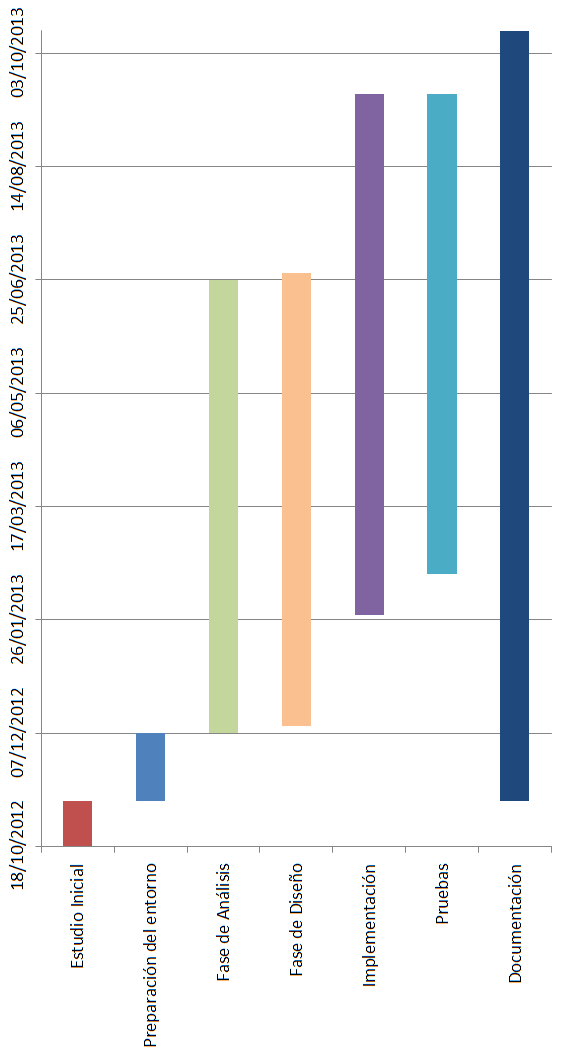
\includegraphics[width=0.7\textwidth]{diagrama_gantt.png}
    \end{center}
    \caption{Diagrama de Gantt con estimación temporal}
    \label{fig:GanttInicial}
\end{figure}

\begin{figure}[H]
    \begin{center}
        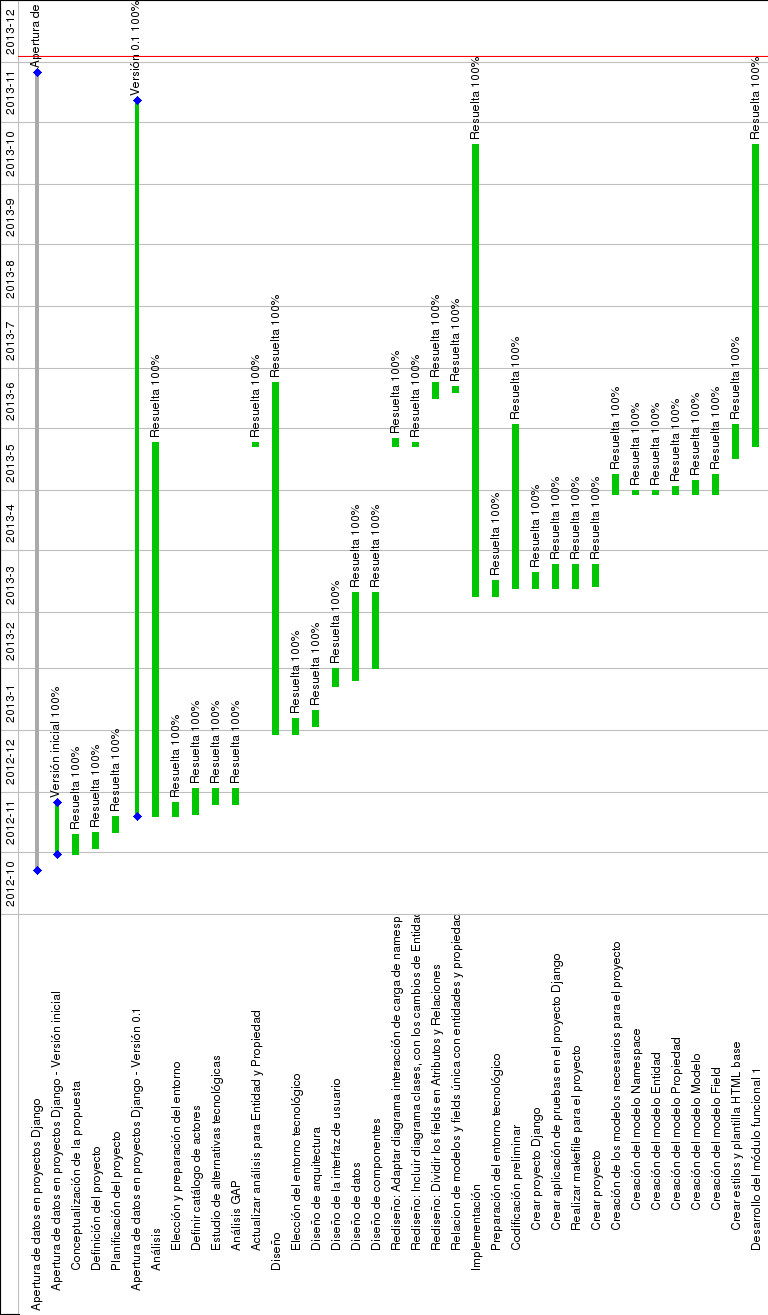
\includegraphics[width=0.85\textwidth]{gantt1.png}
    \end{center}
    \caption{Diagrama de Gantt con los tiempos finales (Parte 1)}
    \label{fig:GanttFinal1}
\end{figure}

\begin{figure}[H]
    \begin{center}
        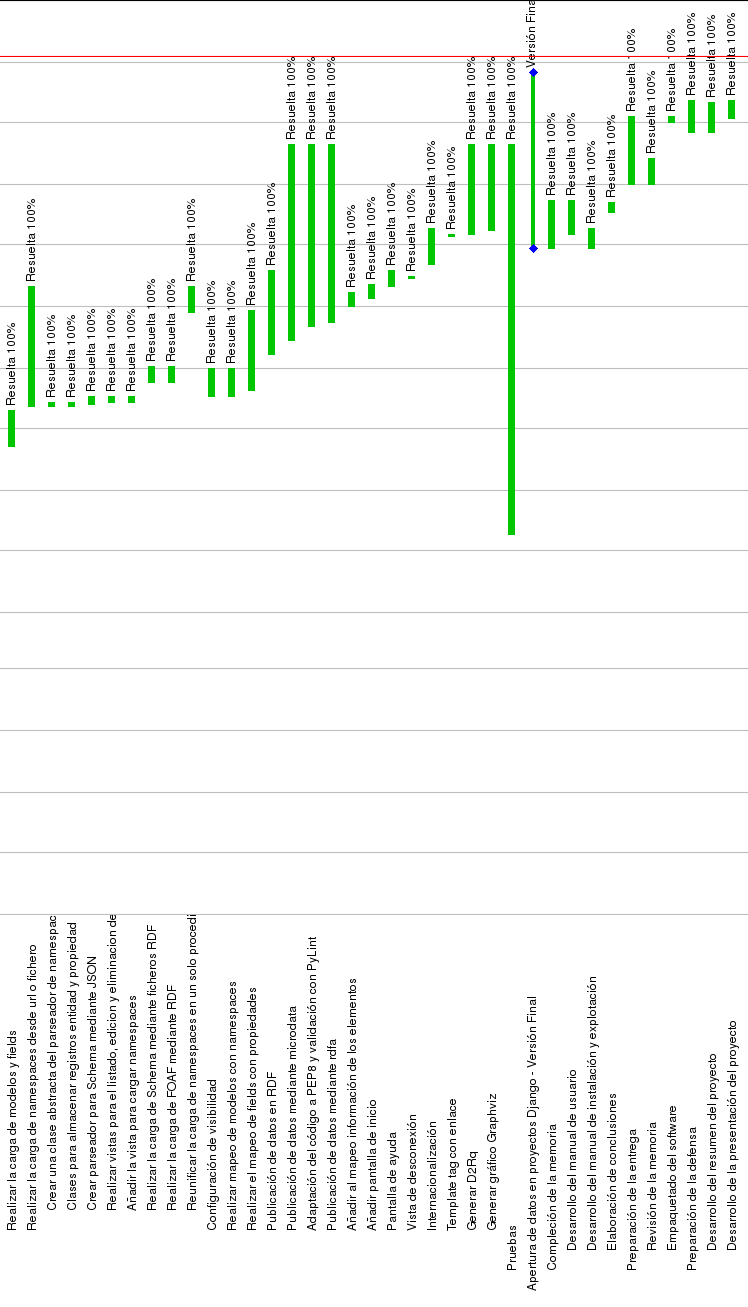
\includegraphics[width=0.85\textwidth]{gantt2.png}
    \end{center}
    \caption{Diagrama de Gantt con los tiempos finales (Parte 2)}
    \label{fig:GanttFinal2}
\end{figure}

\section{Organización}

\section{Roles existentes}

El conjunto de personas que componen a la organización involucrada en el
desarrollo del proyecto, son las siguientes:
\begin{itemize}
    \item \textbf{Desarrollador:} El desarrollador del proyecto, es el alumno
           que está llevando a cabo dicho proyecto informático. Desempeña los
           papeles de analista informático, de desarrollador informático e
           ingeniero de test. Sus funciones son las de analizar y diseñar el
           software, así como de desarrollar el mismo cumpliendo las
           especificaciones, realizar los tests de calidad oportunos y
           documentar todo el proceso de desarrollo.
    \item \textbf{Tutores:} Los tutores del proyectos, tienen como cometido
           guiar al alumno en el desarrollo del mismo. Se puede decir que
           realizan un papel similar al cliente que contrata la realización del
           software, se encargan de proponer el desarrollo del proyecto y de
           proponer los objetivos que debe cumplir el mismo. Además, también
           ayudan al alumno en el proceso de desarrollo, aportando ideas y
           posibles soluciones.
\end{itemize}

Durante el desarrollo del proyecto, el alumno como se acaba de indicar, será el
indicado de realizar todo el proceso del ciclo de vida del software.
Puntualmente, mantendrá reuniones con los tutores del proyecto, de forma que
estos puedan tener una visión del avance del proyecto a lo largo del tiempo. Los
tutores del proyecto, en cada una de estas reuniones, podrán aportar posibles
ideas, o nuevos objetivos que deba cumplir el software, guiando al alumno en la
consecución del mismo.

\section{Recursos inventariables}

En todo proyecto informático, además del factor humano, entran en escena otra
serie de factores, como son los tecnológicos, los cuales servirán al alumno en
la consecución de sus objetivos. En la Tabla \ref{tab:inventario}, se muestra
un inventario de las herramientas, tanto hardware como software, utilizadas
para la elaboración del proyecto:

\begin{center}
    \tablefirsthead{%
        \hline
        \multicolumn{1}{|c|}{\textbf{Recurso inventariable}} &
        \multicolumn{2}{c|}{\textbf{Descripción}} \\
        \hline
    }
    \tablehead{%
        \hline
        \multicolumn{3}{|l|}{\small\sl continuación de la página anterior}\\
        \hline
        \multicolumn{1}{|c|}{\textbf{Elemento inventariable}\hspace{5.5mm}} &
        \multicolumn{2}{c|}{\textbf{Descripción}} \\
        \hline
    }
    \tabletail{%
        \hline
        \multicolumn{3}{|r|}{\small\sl continua en la siguiente página}\\
        \hline
    }
    \tablelasttail{\hline}
    \bottomcaption{Tabla con inventario de materiales}
    \label{tab:inventario}
    \begin{supertabular}{|l@{\hspace{6.5mm}}|l@{\hspace{5.5mm}}|l@{\hspace{5.5mm}}|}
        \multirow{5}{3.5cm}{Hardware} & Procesador & AMD Athlon II x3 460\\
        & Memoria RAM & 8GB DDR3\\
        & Tarjeta Gráfica & NVIDIA GeForce GTX 550 Ti\\
        & Disco Duro & Seagate 1TB SATA3 7200rpm\\
        & Grabadora DVD & LG GH24NS90 DVD 24X\\
        & Monitor & Samsung SyncMaster 2243LNX\\
        \hline
        Sistema operativo & \multicolumn{2}{l|}{Linux Mint 14 Nadia}\\
        \hline
        Editor de textos & \multicolumn{2}{l|}{Gedit 3.4.1}\\
        \hline
        Python & \multicolumn{2}{l|}{Versión 2.7}\\
        \hline
        Django & \multicolumn{2}{l|}{Versión 1.4.0}\\
        \hline
        iPython & \multicolumn{2}{l|}{Interprete interactivo de Python}\\
        \hline
        Dia & \multicolumn{2}{l|}{Software para la generación de gráficos.}\\
        \hline
        Gimp & \multicolumn{2}{l|}{Software para la edición de imágenes.}\\
        \hline
        ConceptDraw Office & \multicolumn{2}{l|}{Software para la generación de diagramas.}\\
        \hline
        Apache & \multicolumn{2}{l|}{Servidor web.}\\
    \end{supertabular}
\end{center}

Para los recursos de tipo software, se ha intentado usar en todo momento
software de tipo libre, de tal forma que se reduzcan los costes al máximo.


\section{Costes}

Para llevar a cabo una estimación de los costes de producción, a parte de tener
una estimación del tiempo y recursos necesarios para llevar a cabo el proyecto,
también es necesario conocer el precio unitario de cada uno de estos recursos.
Si bien, los recursos materiales es de un coste conocido, ya que conocemos de
cuales de ellos necesitamos disponer, y el coste de los mismos. Respecto a
materiales como puede ser el ordenador personal, mobiliario, y demás elementos
de los que debe de poseer cualquier empresa, no deben de tenerse en cuenta su
coste total, ya que estos no son específicos para un puesto en concreto, sino
que se mantendrán en la empresa y su precio se amortizará a lo largo del tiempo.
Normalmente el tiempo de amortización de los mismos, se estima en tres años, por
lo que al haber estimado una duración de un año para el proyecto, contemplaremos
solo un 33\% del precio de los mismos. De esta forma, si suponemos que
conociendo que el coste del equipo informático es de 500\euro, nos quedará un
coste total de 165\euro.

Para estimar el costo de los recursos humanos que intervendrán en el desarrollo
del proryecto software, deberemos de tener en cuenta tanto el número de personas
implicadas, como la duración del proyecto, como el sueldo que habría que
abonarle a cada uno de los participantes en el proyecto. Este proyecto, al
tratarse de un proyecto de pequeña envergadura, será realizado únicamente por
una persona, que trabajará durante 12 meses, que son los que se han estimado
para la duración del proyecto.

En la siguiente Tabla (\ref{tab:costorecursos}) se reflejan los distintos
recursos necesarios para elaborar el proyecto, con los costos y unidades
necesarias asociados de los mismos:

\begin{table}[H]
    \begin{center}
        \begin{tabular}{||c|p{7.5cm}|c||}
            \hline
            \hline
            \textbf{Recurso} & \textbf{Descripción} & \textbf{Coste} \\
            \hline
            \hline
            Ingeniero Informático & Es el encargado de realizar tanto la
            documentación del proyecto, como la implementación del mismo.
            & 1 persona/mes \\
            \hline
            Ordenador Personal & Es el equipo que utilizará el ingeniero
            informático en su puesto de trabajo. & 165\euro \\
            \hline
            Local y mobiliario & Son los gastos del local y derivados del mismo
            (luz, agua, mesa, etc\ldots) donde se va a realizar el proyecto.
            & 30\euro/mes \\
            \hline
            Material de oficina & Hace referencia a papel, bolígrafos,
            etc\ldots & 50\euro \\
            \hline
            \hline
        \end{tabular}
    \end{center}
    \caption{Tabla de costos de los recursos}
    \label{tab:costorecursos}
\end{table}

Una vez conocemos todos los recursos implicados en la elaboración del proyecto,
es necesario tener una estimación del sueldo promedio de un programador
informático en España. Infojobs posee una herramienta \cite{salarioinfo}, la
cual nos permite consultar el sueldo promedio según el puesto de trabajo que
desempeñe el trabajador. Tal y como se puede observar, el salario medio de un
ingeniero informático en España, ronda la cuantía de los \EUR{17567} anuales.
Aunque, para la realización de este proyecto, no se va a tener una dedicación
total, sino que se tratará de una dedicación parcial (aproximadamente una cuarta
parte de lo que dedicaría un trabajador normal), por lo que del total de horas
mensuales que un trabajador normal dispone (alrededor de unas 152 horas),
estimamos que se emplearán aproximadamente unas 38 horas mensuales, de tal forma
que calculando la proporción, nos queda un coste total de \EUR{366} por mes,
para la dedicación que va a tener el ingeniero al proyecto. Finalmente podemos
decir que, si el proyecto tiene un tiempo estimado de 12 meses, y el trabajador
percibirá una cantidad de \EUR{366} cada uno de los meses, el coste total del
trabajador será de \EUR{4.392}.

De esta forma, una vez que conocemos tanto la cantidad como el costo de todos
los recursos implicados en la elaboración del proyecto (tanto humanos como
materiales) y conocemos también la estimación temporal que hicimos
anteriormente, podemos estimar un costo total para el proyecto, el cual se
refleja en la Tabla \ref{tab:costetotal}:

\begin{table}[H]
    \begin{center}
        \begin{tabular}{||c|c|c|c||}
            \hline
            \hline
            \textbf{Unidades} & \textbf{Recurso} & \textbf{Coste unitario} & \textbf{Coste total} \\
            \hline
            \hline
            12 & Ingeniero informático & 366\euro & 4.392\euro \\
            \hline
            1 & Ordenador personal & 165\euro & 165\euro \\
            \hline
            12 & Local & 30\euro & 360\euro \\
            \hline
            1 & Material de oficina & 50\euro & 50\euro \\
            \hline
            \multicolumn{3}{||r|}{\textbf{Total}} & \textbf{4.967\euro} \\
            \hline
            \hline
        \end{tabular}
    \end{center}
    \caption{Tabla de coste total}
    \label{tab:costetotal}
\end{table}

Los costes finales se han calculado en función de 12 meses, ya que en la
planificación que se ha hecho anteriormente y que podemos apreciar en el
diagrama de Gantt (Figura \ref{fig:GanttInicial}), el coste temporal total
comprendía desde Octubre de 2012 hasta Septiembre de 2013, lo que hace un total
de 12 meses.

\section{Gestión de riesgos}

Dentro de todo proyecto, pueden darse a lugar una serie de riesgos, los cuales
complicarían o retrasaría los plazos fijados en la planificación del mismo.
Dentro de estos riesgos, pueden entrar en juego distintos factores, ya sean
humanos o de cualquier otro tipo de índole. En este apartado, vamos a hacer una
descripción de los posibles riesgos que podrían tener lugar, los cuales
comprometiesen el cumplimiento de la planificación. Para la descripción de estos
posibles riesgos, nos vamos a basar en los descritos en el MAGERIT V3
\cite{mageritv3} para determinar los riesgos de tipo genérico que se puedan dar,
y además citaremos otra serie de riesgos específicos del proyecto, los cuales
también retrasarían los plazos estimados en la planificación. Todos estos
riesgos deben de estar descritos dentro de la política de protección de datos de
cualquier empresa.
\begin{itemize}
    \item \textbf{Riesgos de tipo genéricos.}
    \begin{itemize}
        \item \textbf{Errores del administrador (E.2):} equivocaciones de personas
               con responsabilidades de instalación y operación.
        \item \textbf{Destrucción de información (E.18):} perdida de la
               información almacenada del proyecto.
        \item \textbf{Pérdida de equipos (E.25):} la pérdida de equipos provoca
               directamente la carencia de un medio para prestar los servicios,
               es decir una indisponibilidad. 
        \item \textbf{Indisponibilidad del personal (E.28):} ausencia accidental
               del puesto de trabajo: enfermedad, alteraciones del orden público,
               etc\ldots
        \item \textbf{Daños por agua (I.2):} escapes, fugas, inundaciones:
               posibilidad de que el agua acabe con los recursos del sistema.
        \item \textbf{Contaminación mecánica (I.3):} vibraciones, polvo, suciedad,
               \ldots
        \item \textbf{Avería de origen físico o lógico (I.5):} fallos en los
               equipos y/o fallos en los programas. Puede ser debida a un defecto de
               origen o sobrevenida durante el funcionamiento del sistema.
        \item \textbf{Corte del suministro eléctrico (I.6):} cese de la
               alimentación de potencia.
    \end{itemize}
    \item \textbf{Riesgos de tipo específicos del proyecto.}
    \begin{itemize}
        \item \textbf{Cambios en la especificación de los vocabularios:} si se
            introdujesen cambios a la hora de la especificación de los
            vocabularios, haciendo uso de una nomenclatura diferente, habría que
            modificar el parseador de ficheros XML que se encargue de dicha
            función, añadiendo la nueva nomenclatura.
        \item \textbf{Cambios en la estructura de la base de datos:} si por la
            aparición de nuevas necesidades o por deficiencias en la estuctura
            actual se debiesen hacer cambios en la base de datos, se debería de
            volver nuevamente al apartado de diseño, para definir la nueva
            estructura de la misma, determinar los sistemas donde afectarán
            dichos cambios y si fuese necesario, definir herramientas de
            migración de los datos a las nuevas estructuras, para evitar la
            pérdida de datos.
        \item \textbf{Modificación de funcionalidades existentes:} si alguna de
            las funcionalidades especificadas en el proyecto se modificasen, se
            debería de volver al apartado de análisis y diseño, para modificar
            los diagramas de caso de uso e interacción de dicha funcionalidad,
            para posteriormente pasar a la modificación de la funcionalidad.
    \end{itemize}
\end{itemize}

Para la subsanación de los riesgos que provocan una pérdida de datos, o un
deterioro de los mismos, como son los riesgos marcados con los códigos E.2,
E.18, E.25, I.2, I.3, I.5 e I.6, se hará uso de un sistema de control de 
versiones (en
nuestro caso se hace uso del sistema subversion), el cual permita en todo
momento mantener una copia de cada una de las versiones que existen del proyecto,
garantizando la disponibilidad e integridad de los datos. Asímismo, este
sistema de control de versiones, se encontrará en otra máquina ajena a la
máquina donde se está desarrollando el proyecto, y en un edificio distinto. De
esta forma, evitamos posibles pérdidas de información por causas naturales,
subidas de tensión, o deterioro de componentes físicos de la máquina donde se
está realizando el proyecto.

En el ámbito de los riesgos provocados por causas humanas, debidas a la
indisponibilidad del persona, al tratarse de un equipo de desarrollo bastante
reducido, compuesto únicamente por una persona, las precauciones que se han
tomando, han sido las de contemplar las posibles bajas por enfermedad o
indisponibilidad por parte del personal, dentro de los plazos estipulados de
realización del proyecto, intentando ajustar los plazos siempre todo lo posible,
pero dando siempre cierto margen en los tiempos (teniendo siempre en cuenta que
los costes y tiempos se encuentren siempre dentro de límites razonables), de tal
forma que un posible contratiempo de este tipo, no altere de sobremanera los
tiempos de entrega, prologándolos demasiado en el tiempo.



% DESARROLLO
\part{Desarrollo}
%\null\vfill
%\noindent En esta parte se debe describir el desarrollo del proyecto siguiendo la metodología empleada. Sus capítulos no deben ser una descripción exhaustiva de todos los documentos, diagramas, código fuente y, en general, entregables generados, sino más bien una explicación resumida del desarrollo, estructurada según las etapas principales del proceso de ingeniería. Deben seleccionarse aquellos diagramas, fragmentos de código y secciones de los entregables que sean más significativos para dicha explicación. La totalidad de los entregables resultado del proyecto se ubicarán en los anexos y/o en el material en CD/DVD que acompañe al proyecto.


\chapter{Análisis de Requisitos}
% ------------------------------------------------------------------------------
% Este fichero es parte de la plantilla LaTeX para la realización de Proyectos
% Final de Grado, protegido bajo los términos de la licencia GFDL.
% Para más información, la licencia completa viene incluida en el
% fichero fdl-1.3.tex

% Copyright (C) 2012 SPI-FM. Universidad de Cádiz
% ------------------------------------------------------------------------------

En esta sección se presenta el catálogo de requisitos del sistema de
información. Para ello se detallarán los actores del sistema, los requisitos
funcionales, los requisitos de información, los requisitos no funcionales y las
reglas de negocio. Luego se describen las diferentes alternativas tecnológicas y
el análisis de la brecha entre los requisitos planteados y la solución base
seleccionada.

\section{Catálogo de actores}

Dentro del funcionamiento de la aplicación, intervienen una serie de actores,
los cuales son los encargados de activar cada una de las operaciones de las que
dispone la aplicación. Estos actores, los cuales intervienen dentro de los casos
de uso de la aplicación, son los que se describen a continuación:

\subsection{Administrador del sistema}

%%%TABLA - Actor Administrador del sistema
\begin{center}
\begin{longtable}{||p{3.4cm}|p{12cm}||}
%primera parte de la tabla
 \hline \hline \bf ACT-001 &  \bf Administrador del sistema \\
\hline
\endfirsthead
%primera parte de la tabla por pagina
\hline \multicolumn{2}{|r|}{{Continuación de la tabla}} \\ \hline
 \hline \bf ACT-001 &  \bf Administrador del sistema \\
\hline
\endhead
% ultima parte de la tabla por pagina
\hline \multicolumn{2}{|l|}{{Continúa en la siguiente página}} \\ \hline
\endfoot
% ultima parte de la tabla
\endlastfoot
% DATOS
 \hline \bf Descripción & El actor administrador representa a toda
             aquella persona con acceso a la aplicación, que cuente con permisos
             de superusuario. Este actor es el encargado de la configuración y
             administración de la aplicación.\\
\hline
\hline
\caption{\label{tab:act001} Actor - 001 - Administrador del sistema} 
\end{longtable}
\end{center}


\subsection{Usuario externo}

%%%TABLA - Actor Usuario externo
\begin{center}
\begin{longtable}{||p{3.4cm}|p{12cm}||}
%primera parte de la tabla
 \hline \hline \bf ACT-002 &  \bf Usuario externo \\
\hline
\endfirsthead
%primera parte de la tabla por pagina
\hline \multicolumn{2}{|r|}{{Continuación de la tabla}} \\ \hline
 \hline \bf ACT-002 &  \bf Usuario externo \\
\hline
\endhead
% ultima parte de la tabla por pagina
\hline \multicolumn{2}{|l|}{{Continúa en la siguiente página}} \\ \hline
\endfoot
% ultima parte de la tabla
\endlastfoot
% DATOS
 \hline \bf Descripción & El actor Usuario externo (persona o sistema)
             representa a toda aquella persona externa al proyecto donde va a
             ser usada la aplicación, de forma que vaya a hacer uso de los
             recursos públicos de ella, cuando acceda a la misma.\\
\hline
\hline
\caption{\label{tab:act002} Actor - 002 - Usuario externo} 
\end{longtable}
\end{center}


\section{Requisitos funcionales}

A continuación se realiza una descripción de los distintos requisitos
funcionales que deberá de cumplir la aplicación. Se van a describir cada uno de
estos requisitos funcionales como casos de uso, donde mostraremos los actores
implicados en el desarrollo de los mismos, así como las precondiciones,
postcondiciones y los posibles escenarios alternativos que se puedan dar.

Primeramente vamos a mostrar los diagramas de Casos de Uso, para posteriormente
pasar a la descripción de cada uno de estos. Los casos de usos los dividiremos
en dos grupos, aquellos que pertenecen al subsistema del administrador (las
operaciones que el administrador y solo el administrador debe poder hacer) y el
subsistema perteneciente al usuario externo (estas operaciones podrán ser
realizadas por cualquier usuario).

\subsection{Diagramas de Casos de Uso}

\subsubsection{Casos de Uso del Usuario externo}

\begin{figure}[H]
    \begin{center}
        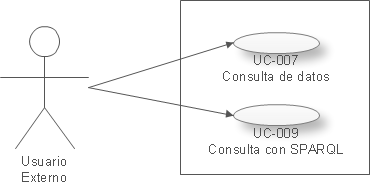
\includegraphics[width=0.6\textwidth]{diagramas_cu/CU_UExterno.png}
    \end{center}
    \caption{Diagrama de CU del Usuario externo}
    \label{fig:DCUAdministrador}
\end{figure}

\subsubsection{Casos de Uso del Administrador}

\begin{figure}[H]
    \begin{center}
        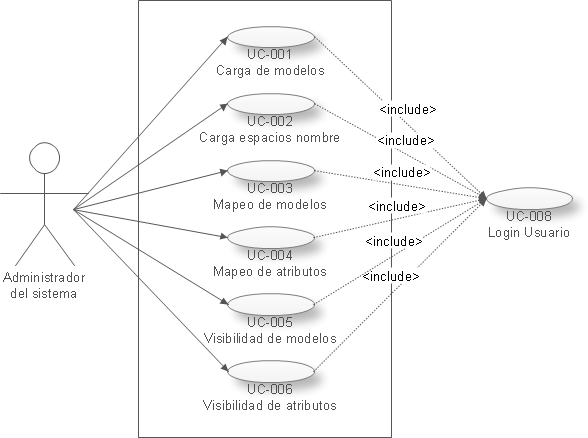
\includegraphics[width=0.8\textwidth]{diagramas_cu/CU_Administrador.png}
    \end{center}
    \caption{Diagrama de CU del Administrador}
    \label{fig:DCUAdministrador}
\end{figure}


\subsection{Descripción de los Casos de Uso}

En este apartado, realizamos una descripción a fondo de cada uno de los Casos de
Uso mostrados anteriormente. Para cada uno de ellos, indicamos los actores que
intervienen en el, la descripción del mismo, posibles flujos alternativos que
puedan darse, y así como la descripción de precondiciones y postcondiciones que
deberán de cumplirse.

\subsubsection{Carga de modelos}

%%%TABLA - Caso de uso 001
\begin{center}
\begin{longtable}{||p{3.4cm}|p{12cm}||}
%primera parte de la tabla
 \hline \hline \bf UC-001 &  \bf Carga de modelos \\
\hline
\endfirsthead
%primera parte de la tabla por pagina
\hline \multicolumn{2}{|r|}{{Continuación de la tabla}} \\ \hline
 \hline \bf UC-001 &  \bf Carga de modelos \\
\hline
\endhead
% ultima parte de la tabla por pagina
\hline \multicolumn{2}{|l|}{{Continúa en la siguiente página}} \\ \hline
\endfoot
% ultima parte de la tabla
\endlastfoot
% DATOS
 \hline \bf Descripción & Carga de modelos y fields del proyecto Django
             donde se va a usar la aplicación.\\
 \hline \bf Referencia & Tabla \ref{tab:caso001}\\
\hline
\hline
\caption{\label{tab:caso001-red} Descripción Caso de Uso - 001 - Carga de modelos} 
\end{longtable}
\end{center}


\subsubsection{Carga de espacios de nombres}

%%%TABLA - Caso de uso 002
\begin{center}
\begin{longtable}{||p{3.4cm}|p{12cm}||}
%primera parte de la tabla
 \hline \hline \bf UC-002 &  \bf Carga de espacios de nombres \\
\hline
\endfirsthead
%primera parte de la tabla por pagina
\hline \multicolumn{2}{|r|}{{Continuación de la tabla}} \\ \hline
 \hline \bf UC-002 &  \bf Carga de espacio de nombres \\
\hline
\endhead
% ultima parte de la tabla por pagina
\hline \multicolumn{2}{|l|}{{Continúa en la siguiente página}} \\ \hline
\endfoot
% ultima parte de la tabla
\endlastfoot
% DATOS
 \hline \bf Descripción & Se debe de realizar una serie de procedimientos los
             cuales permitan a la aplicación cargar la estructura de los
             diferentes namespaces existentes, además de permitir actualizar y
             eliminar estos.\\
 \hline \bf Referencia & Tabla \ref{tab:caso002}\\
\hline
\hline
\caption{\label{tab:caso002-red} Descripción Caso de Uso - 002 - Carga de espacios de nombres}
\end{longtable}
\end{center}


\subsubsection{Mapeo de modelos}

%%%TABLA - Caso de uso 003
\begin{center}
\begin{longtable}{||p{3.4cm}|p{12cm}||}
%primera parte de la tabla
 \hline \hline \bf UC-003 &  \bf Mapeo de modelos \\
\hline
\endfirsthead
%primera parte de la tabla por pagina
\hline \multicolumn{2}{|r|}{{Continuación de la tabla}} \\ \hline
 \hline \bf UC-003 &  \bf Mapeo de modelos \\
\hline
\endhead
% ultima parte de la tabla por pagina
\hline \multicolumn{2}{|l|}{{Continúa en la siguiente página}} \\ \hline
\endfoot
% ultima parte de la tabla
\endlastfoot
% DATOS
 \hline \bf Descripción & Este caso de uso describe el procedimiento mediante
             el cual el administrador del sistema, describe en la aplicación la
             relación de cada uno de los modelos del proyecto Django, con las
             entidades de los distintos namespaces que existen en la
             aplicación.\\
 \hline \bf Referencia & Tabla \ref{tab:caso003}\\
\hline
\hline
\caption{\label{tab:caso003-red} Descripción Caso de Uso - 003 - Mapeo de \mbox{modelos}} 
\end{longtable}
\end{center}


\subsubsection{Mapeo de los atributos}

%%%TABLA - Caso de uso 004
\begin{center}
\begin{longtable}{||p{3.4cm}|p{12cm}||}
%primera parte de la tabla
 \hline \hline \bf UC-004 &  \bf Mapeo de los atributos \\
\hline
\endfirsthead
%primera parte de la tabla por pagina
\hline \multicolumn{2}{|r|}{{Continuación de la tabla}} \\ \hline
 \hline \bf UC-004 &  \bf Mapeo de los atributos \\
\hline
\endhead
% ultima parte de la tabla por pagina
\hline \multicolumn{2}{|l|}{{Continúa en la siguiente página}} \\ \hline
\endfoot
% ultima parte de la tabla
\endlastfoot
% DATOS
 \hline \bf Descripción & Este caso de uso describe el procedimiento mediante
             el cual el administrador del sistema, describe en la aplicación la
             relación de cada uno de los atributos de los modelos del proyecto
             Django, con las propiedades de las entidades de los distintos
             namespaces que existen en la aplicación.\\
 \hline \bf Referencia & Tabla \ref{tab:caso004}\\
\hline
\hline
\caption{\label{tab:caso004-red} Descripción Caso de Uso - 004 - Mapeo de los atributos} 
\end{longtable}
\end{center}


\subsubsection{Establecer visibilidad de modelos}

%%%TABLA - Caso de uso 005
\begin{center}
\begin{longtable}{||p{3.4cm}|p{12cm}||}
%primera parte de la tabla
 \hline \hline \bf UC-005 &  \bf Establecer visibilidad de modelos \\
\hline
\endfirsthead
%primera parte de la tabla por pagina
\hline \multicolumn{2}{|r|}{{Continuación de la tabla}} \\ \hline
 \hline \bf UC-005 &  \bf Establecer visibilidad de modelos \\
\hline
\endhead
% ultima parte de la tabla por pagina
\hline \multicolumn{2}{|l|}{{Continúa en la siguiente página}} \\ \hline
\endfoot
% ultima parte de la tabla
\endlastfoot
% DATOS
 \hline \bf Descripción & Este caso de uso describe el procedimiento que debe
             de seguir el administrador del sistema, para especificar aquellos
             modelos del proyecto Django de los que podrán publicarse los datos.\\
 \hline \bf Referencia & Tabla \ref{tab:caso005}\\
\hline
\hline
\caption{\label{tab:caso005-red} Descripción Caso de Uso - 005 - Establecer visibilidad de modelos} 
\end{longtable}
\end{center}


\subsubsection{Establecer visibilidad de los atributos}

%%%TABLA - Caso de uso 006
\begin{center}
\begin{longtable}{||p{3.4cm}|p{12cm}||}
%primera parte de la tabla
 \hline \hline \bf UC-006 &  \bf Establecer visibilidad de los atributos\\
\hline
\endfirsthead
%primera parte de la tabla por pagina
\hline \multicolumn{2}{|r|}{{Continuación de la tabla}} \\ \hline
 \hline \bf UC-006 &  \bf Establecer visibilidad de los atributos \\
\hline
\endhead
% ultima parte de la tabla por pagina
\hline \multicolumn{2}{|l|}{{Continúa en la siguiente página}} \\ \hline
\endfoot
% ultima parte de la tabla
\endlastfoot
% DATOS
 \hline \bf Descripción & Este caso de uso describe el procedimiento que debe
             de seguir el administrador del sistema, para especificar aquellos
             atributos de los modelos del proyecto Django de los que podrán
             publicarse los datos.\\
 \hline \bf Referencia & Tabla \ref{tab:caso006}\\
\hline
\hline
\caption{\label{tab:caso006-red} Descripción Caso de Uso - 006 - Establecer visibilidad atributos} 
\end{longtable}
\end{center}


\subsubsection{Publicación de los datos}

%%%TABLA - Caso de uso 007
\begin{center}
\begin{longtable}{||p{3.4cm}|p{12cm}||}
%primera parte de la tabla
 \hline \hline \bf UC-007 &  \bf Consulta de datos \\
\hline
\endfirsthead
%primera parte de la tabla por pagina
\hline \multicolumn{2}{|r|}{{Continuación de la tabla}} \\ \hline
 \hline \bf UC-007 &  \bf Consulta de datos \\
\hline
\endhead
% ultima parte de la tabla por pagina
\hline \multicolumn{2}{|l|}{{Continúa en la siguiente página}} \\ \hline
\endfoot
% ultima parte de la tabla
\endlastfoot
% DATOS
 \hline \bf Descripción & Muestra los datos por pantalla usando los estándares
    RDF/XML, RDF/Ntriples, RDF/Turtle, RDFa o Microdata, existentes para la
    publicación de datos en internet.\\
 \hline \bf Referencia & Tabla \ref{tab:caso007}\\
\hline
\hline
\caption{\label{tab:caso007-red} Descripción Caso de Uso - 007 - Consulta de datos} 
\end{longtable}
\end{center}


\subsubsection{Inicio de sesión}

%%%TABLA - Caso de uso 008
\begin{center}
\begin{longtable}{||p{3.4cm}|p{12cm}||}
%primera parte de la tabla
 \hline \hline \bf UC-008 &  \bf Inicio de sesión \\
\hline
\endfirsthead
%primera parte de la tabla por pagina
\hline \multicolumn{2}{|r|}{{Continuación de la tabla}} \\ \hline
 \hline \bf UC-008 &  \bf Inicio de sesión \\
\hline
\endhead
% ultima parte de la tabla por pagina
\hline \multicolumn{2}{|l|}{{Continúa en la siguiente página}} \\ \hline
\endfoot
% ultima parte de la tabla
\endlastfoot
% DATOS
 \hline \bf Descripción & Realiza el login del usuario dentro de la aplicación
        web.\\
 \hline \bf Referencia & Tabla \ref{tab:caso008}\\
\hline
\hline
\caption{\label{tab:caso008-red} Descripción Caso de Uso - 008 - Inicio de sesión} 
\end{longtable}
\end{center}


\subsubsection{Consulta con SPARQL}

%%%TABLA - Caso de uso 009
\begin{center}
\begin{longtable}{||p{3.4cm}|p{12cm}||}
%primera parte de la tabla
 \hline \hline \bf UC-009 &  \bf Consulta con SPARQL \\
\hline
\endfirsthead
%primera parte de la tabla por pagina
\hline \multicolumn{2}{|r|}{{Continuación de la tabla}} \\ \hline
 \hline \bf UC-009 &  \bf Consulta con SPARQL \\
\hline
\endhead
% ultima parte de la tabla por pagina
\hline \multicolumn{2}{|l|}{{Continúa en la siguiente página}} \\ \hline
\endfoot
% ultima parte de la tabla
\endlastfoot
% DATOS
 \hline \bf Descripción & Debe de permitirse al usuario realizar consultas sobre
        los datos utilizando el lenguaje SPARQL.\\
 \hline \bf Referencia & Tabla \ref{tab:caso009}\\
\hline
\hline
\caption{\label{tab:caso009-red} Descripción Caso de Uso - 009 - Consulta con SPARQL} 
\end{longtable}
\end{center}


\subsection{Diagramas de Secuencia}

Una vez hemos descrito cada uno de los casos de uso que deberá incluir la
aplicación, el siguiente paso es plasmar gráficamente el comportamiento de
estos. De esta forma, se muestran a continuación, los diagramas de secuencia de
cada uno de los casos de uso de la aplicación.

\newpage

\subsubsection{UC-001 }

\begin{figure}[H]
    \begin{center}
        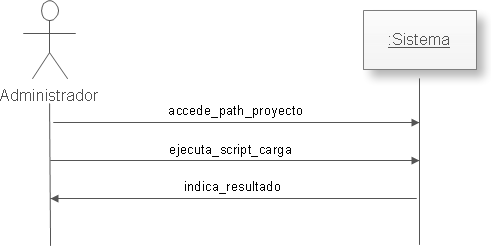
\includegraphics[width=0.75\textwidth]{diagramas_secuencia/DiagramasSecuencia-001.png}
    \end{center}
    \caption{Diagrama de Secuencia CU-001}
    \label{fig:DSCU-001}
\end{figure}

\subsubsection{UC-002 }

\begin{figure}[H]
    \begin{center}
        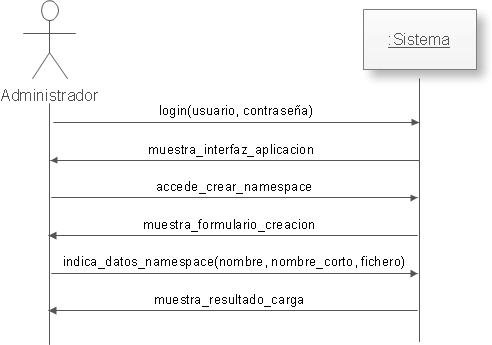
\includegraphics[width=0.7\textwidth]{diagramas_secuencia/DiagramasSecuencia-002.png}
    \end{center}
    \caption{Diagrama de Secuencia CU-002}
    \label{fig:DSCU-002}
\end{figure}

\subsubsection{UC-003 }

\begin{figure}[H]
    \begin{center}
        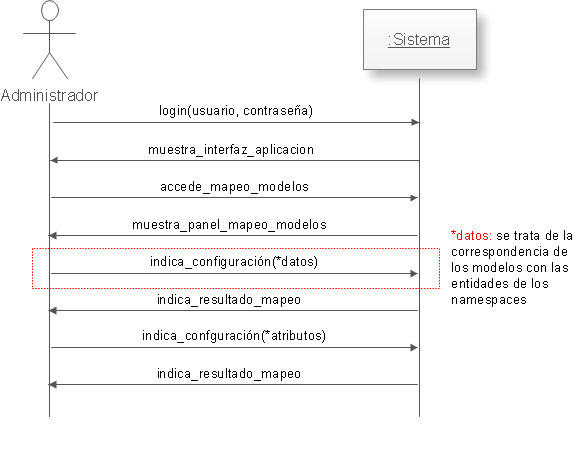
\includegraphics[width=0.7\textwidth]{diagramas_secuencia/DiagramasSecuencia-003.png}
    \end{center}
    \caption{Diagrama de Secuencia CU-003}
    \label{fig:DSCU-003}
\end{figure}

\subsubsection{UC-004 }

\begin{figure}[H]
    \begin{center}
        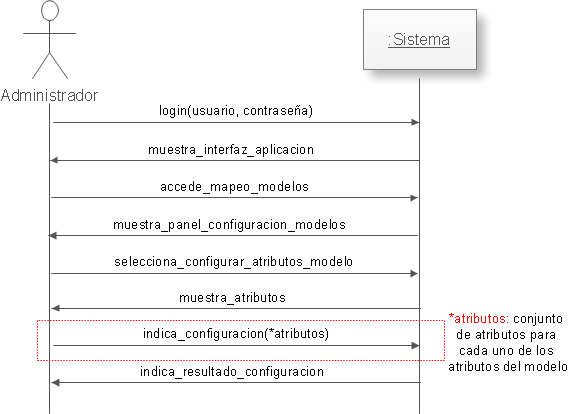
\includegraphics[width=0.7\textwidth]{diagramas_secuencia/DiagramasSecuencia-004.png}
    \end{center}
    \caption{Diagrama de Secuencia CU-004}
    \label{fig:DSCU-004}
\end{figure}

\subsubsection{UC-005 }

\begin{figure}[H]
    \begin{center}
        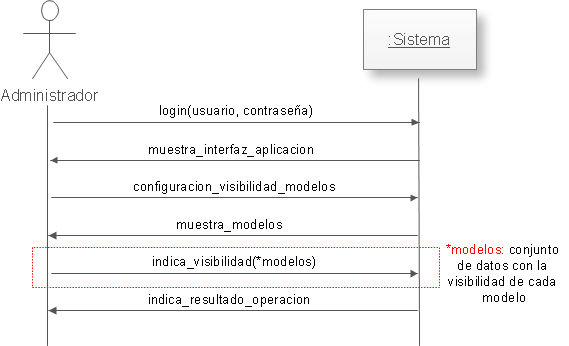
\includegraphics[width=0.75\textwidth]{diagramas_secuencia/DiagramasSecuencia-005.png}
    \end{center}
    \caption{Diagrama de Secuencia CU-005}
    \label{fig:DSCU-005}
\end{figure}

\subsubsection{UC-006 }

\begin{figure}[H]
    \begin{center}
        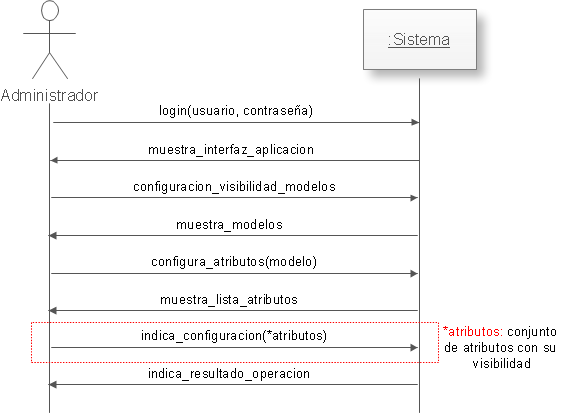
\includegraphics[width=0.8\textwidth]{diagramas_secuencia/DiagramasSecuencia-006.png}
    \end{center}
    \caption{Diagrama de Secuencia CU-006}
    \label{fig:DSCU-006}
\end{figure}
\newpage

\subsubsection{UC-007 }

\begin{figure}[H]
    \begin{center}
        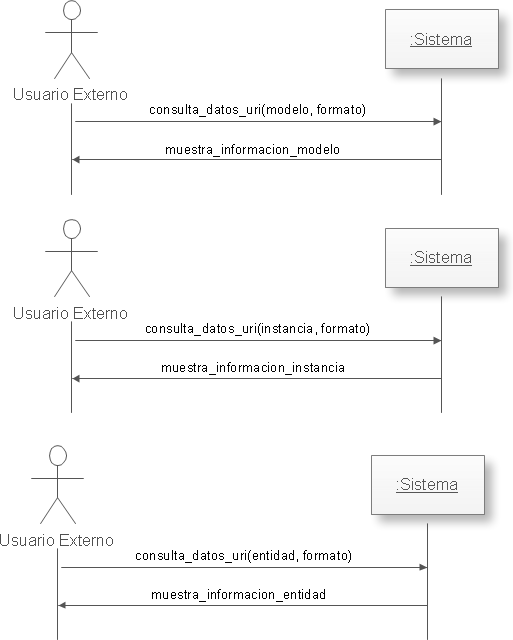
\includegraphics[width=0.8\textwidth]{diagramas_secuencia/DiagramasSecuencia-007.png}
    \end{center}
    \caption{Diagrama de Secuencia CU-007}
    \label{fig:DSCU-007}
\end{figure}

\newpage

\subsubsection{UC-008 }

\begin{figure}[H]
    \begin{center}
        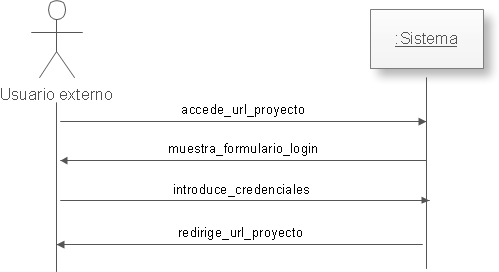
\includegraphics[width=0.8\textwidth]{diagramas_secuencia/DiagramasSecuencia-008.png}
    \end{center}
    \caption{Diagrama de Secuencia CU-008}
    \label{fig:DSCU-008}
\end{figure}

\subsubsection{UC-009 }

\begin{figure}[H]
    \begin{center}
        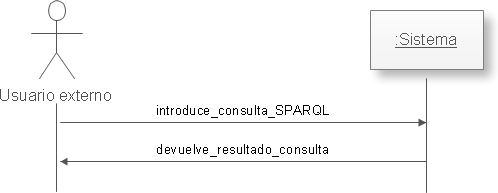
\includegraphics[width=0.8\textwidth]{diagramas_secuencia/DiagramasSecuencia-009.png}
    \end{center}
    \caption{Diagrama de Secuencia CU-009}
    \label{fig:DSCU-009}
\end{figure}


\section{Requisitos de información}

En esta sección se describen los requisitos de gestión de información (datos)
que el sistema debe gestionar. Para ello, utilizando el formato de
especificación propuesto por UML, detallamos a continuación, cada uno de los
requisitos de información de la aplicación:

\subsection{Descripción de los requisitos de información}

%%%TABLA - Requisito Información de los namespaces
\begin{center}
\begin{longtable}{||p{3.4cm}|p{12cm}||}
%primera parte de la tabla
 \hline \hline \bf IRQ-001 &  \bf Información de los namespaces \\
\hline
\endfirsthead
%primera parte de la tabla por pagina
\hline \multicolumn{2}{|r|}{{Continuación de la tabla}} \\ \hline
 \hline \bf IRQ-001 &  \bf Información de los namespaces \\
\hline
\endhead
% ultima parte de la tabla por pagina
\hline \multicolumn{2}{|l|}{{Continúa en la siguiente página}} \\ \hline
\endfoot
% ultima parte de la tabla
\endlastfoot
% DATOS
 \hline \bf Descripción & Se debe almacenar la información acerca de los
             distintos namespaces que almacena la aplicación, de tal forma que
             se tenga la información acerca del namespace, de las entidades que
             componen a este, y de las propiedades que componen a la entidad.\\
 \hline \bf Referencia & Tabla \ref{tab:irq001}\\
\hline
\hline
\caption{\label{tab:irq001-red} Descripción IRQ - 001 - Información de los namespaces} 
\end{longtable}
\end{center}

%%%TABLA - Requisito Información de los modelos
\begin{center}
\begin{longtable}{||p{3.4cm}|p{12cm}||}
%primera parte de la tabla
 \hline \hline \bf IRQ-002 &  \bf Información de los modelos \\
\hline
\endfirsthead
%primera parte de la tabla por pagina
\hline \multicolumn{2}{|r|}{{Continuación de la tabla}} \\ \hline
 \hline \bf IRQ-002 &  \bf Información de los modelos \\
\hline
\endhead
% ultima parte de la tabla por pagina
\hline \multicolumn{2}{|l|}{{Continúa en la siguiente página}} \\ \hline
\endfoot
% ultima parte de la tabla
\endlastfoot
% DATOS
 \hline \bf Descripción & Se debe almacenar la información acerca de los
             distintos modelos que componen al proyecto Django, de tal forma que
             se tenga la información acerca del modelo, y de los fields que
             componen al modelo.\\
 \hline \bf Referencia & Tabla \ref{tab:irq002}\\
\hline
\hline
\caption{\label{tab:irq002-red} Descripción IRQ - 002 - Información de los modelos} 
\end{longtable}
\end{center}


\subsection{Diagrama conceptual de datos}

Una vez que hemos descrito cada uno de los datos que necesitamos que nuestra
aplicación Django almacene, mostramos un diagrama conceptual de datos UML,
donde se puede apreciar como se relacionan cada uno de estos datos entre ellos.
Además, a parte de las distintas clases que almacena la aplicación, podremos
identificar, los atributos, relaciones y restricciones adicionales.

Si observamos el diagrama de clases, está divido en dos partes, numeradas cada
una de ellas. La parte número 1, se corresponde con el requisito de información
\textit{IRQ-001} (Tabla \ref{tab:irq001}), y el apartado número 2, se
corresponde con los requisitos de información descritos en \textit{IRQ-002}
(Tabla \ref{tab:irq002}).

\newpage

\begin{figure}[H]
    \begin{center}
        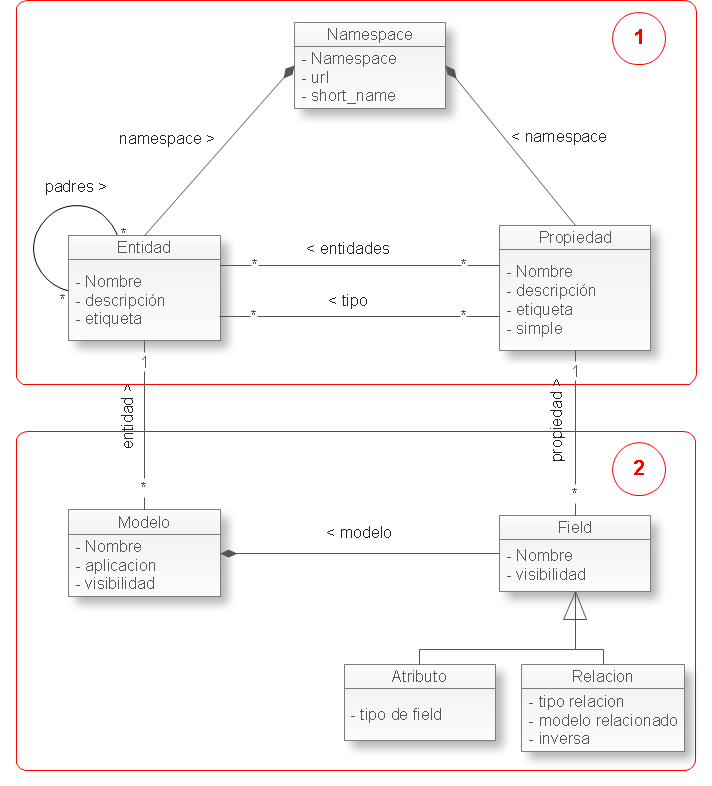
\includegraphics[width=0.9\textwidth]{diagrama_clases.png}
    \end{center}
    \caption{Diagrama conceptual de datos UML}
    \label{fig:ClasesUML}
\end{figure}

\section{Requisitos no funcionales}
\label{sec:RQNF}

A continuación se detalla una descripción de otra serie requisitos, relacionados
con la calidad del software, conocidos como requisitos no funcionales, que el
sistema deberá satisfacer. Estos requisitos son los siguientes:
\begin{itemize}
    \item \textbf{Seguridad:} dicha aplicación no será accesible a usuarios no
           autorizados y solo se publicarán aquellos datos expresamente
           indicados.
    \item \textbf{Estándares de las organizaciones:} deberá de adaptarse a
           cada uno de los estándares impuestos por las distintas organizaciones
           desarrolladoras de las especificaciones para la apertura de datos.
    \item \textbf{Portabilidad:} la aplicación debe de estar diseñada,
           haciendo uso siempre de tecnologías y herramientas independientes de
           la plataforma, de forma que pueda usarse bajo la gran mayoría de
           sistemas operativos actuales.
    \item \textbf{Mantenibilidad:} Esta aplicación se encuentra desarrollada
           como un módulo a parte, de forma que no sea dependiente de un
           proyecto en cuestión. Además, la aplicación deberá de estar
           perfectamente documentada, y se usará la guía de buenas maneras para
           la escritura de código Python PEP8 (\cite{pep8}), de tal forma que
           el código sea lo suficientemente claro.
    \item \textbf{Extensibilidad:} La aplicación debe de ser fácilmente
           extensible, pudiéndose adaptar fácilmente a nuevos estándares para la
           apertura de datos.
    \item \textbf{Interfaz:} La aplicación debe de poseer una interfaz de
           configuración sencilla e intuitiva, de tal forma que un usuario no
           experimentado, pueda aprender a manejarla sin dificultades.
    \item \textbf{Entorno tecnológico:} La aplicación forzosamente debe de
           estar elaborada bajo el lenguaje de programación Python y el
           framework Django, ya que es el principal objetivo de este proyecto,
           proporcionar una herramienta para la apertura de datos en
           aplicaciones Django. El resto de tecnologías a usar, es indiferente,
           siempre y cuando respeten los requisitos que se acaban de imponer.
\end{itemize}


\section{Reglas de negocio}

A lo largo del desarrollo del sistema, además de los distintos requisitos que ha
de cumplir la aplicación, en lo referente a funcionalidades, información o
propiedades que deben de cumplir el sistema, hay que tener en cuenta las
denominadas reglas de negocio, es decir, el conjunto de restricciones, normas o
políticas de la organización que deben ser respetadas por el sistema. A
continuación se detallan, una lista de las distintas reglas de negocio que debe
de cumplir la aplicación:
\begin{enumerate}
    \item El sistema no debe de permitir que un usuario que no posea los
           permisos de administrador, pueda consultar datos, los cuales están
           declarados como privados.
    \item El sistema no permitirá acceder al apartado de configuración de la
           publicación de datos a usuarios que no posean credenciales de
           administrador.
\end{enumerate}

\section{Estudio de alternativas tecnológicas}

La finalidad de este apartado, sería de comentar las diferentes alternativas
tecnológicas que existen, las cuales nos permitirían obtener el producto que
queremos desarrollar, comentando posibles pros y contras de cada una de estas,
de forma que nos ayude a decidirnos por cual de ellas sería la mejor. Aunque en
nuestro caso, no será necesario definir estas, ya que el principal objetivo de
este proyecto informático, es el de dotar de una cierta cualidad (apertura de
datos en internet) a una tecnología en concreto (Django), por lo que no tendría
sentido en un principio estudiar otras alternativas tecnológicas.

\section{Análisis GAP}

Este proyecto no se encuentra basado en ningún software base, ya que vamos a
realizar una aplicación software completamente desde cero. Si cabe comentar, que
el proyecto se va a realizar en Python, para el framework Django, por lo que si
considerásemos el framework Django como un software base a partir del cual vamos
a desarrollar nuestro proyecto, este nos proporciona una serie de herramientas
las cuales nos simplificarán el desarrollo del mismo. Entre todas estas
herramientas que comentamos, cabría destacar las siguientes:
\begin{itemize}
    \item Herramientas para el acceso a los distintos modelos de las
           aplicaciones. Esto nos facilitará enormemente la introspección que
           deberemos de realizar, para captar los modelos de los que se
           encuentran compuestos los proyectos Django.
    \item Herramientas para la gestión de las sesiones y del log de la
           aplicación.
    \item Herramientas para la generación de formularios, incluyendo
           comprobaciones de seguridad ante distintos tipos de ataques.
    \item Manejador propio para las bases de datos, con un lenguaje propio de
           consultas, de tal forma que podemos realizar la aplicación de forma
           que esta sea completamente independiente del SGBD que use el proyecto
           donde vaya a ser implantada la aplicación.
    \item Una comunidad, la cual proporciona un soporte continuo del framework
           Django.
\end{itemize}

El proyecto aunque no toma como base para su desarrollo la plataforma D2Rq,
genera ficheros de configuración para ésta, por lo que para el desarrollo de
este módulo se ha debido de realizar un estudio del funcionamiento de esta
plataforma, y adaptar la generación del fichero de configuración a ésta. La
plataforma D2Rq, es de código abierto, y proporciona un sistema para el acceso a
los datos de bases de datos relacionales, como si se tratasen de grafos RDF
virtuales de solo lectura. De esta forma, ofrece a los usuario acceso mediante
RDF al contenido relacional de las bases de datos, sin la necesidad de tener que
replicar estos sobre un almacenamiento en formato RDF.


\chapter{Diseño del Sistema}
% ------------------------------------------------------------------------------
% Este fichero es parte de la plantilla LaTeX para la realización de Proyectos
% Final de Grado, protegido bajo los términos de la licencia GFDL.
% Para más información, la licencia completa viene incluida en el
% fichero fdl-1.3.tex

% Copyright (C) 2012 SPI-FM. Universidad de Cádiz
% ------------------------------------------------------------------------------

En este capítulo se recoge la arquitectura general del sistema de información,
el diseño de la interfaz de usuario, el diseño físico de datos, el diseño de
componentes software y la parametrización del software base.

\section{Diseño de la arquitectura}
En esta sección se define la arquitectura general del sistema de información,
especificando las distintas particiones físicas del mismo, la descomposición
lógica en subsistemas de diseño y la ubicación de cada subsistema en cada
partición, así como la especificación detallada de la infraestructura
tecnológica necesaria para dar soporte al sistema de información.

\subsection{Arquitectura física}

En este apartado, describimos los principales componentes hardware que forman la
arquitectura física de nuestro sistema, recogiendo por un lado los componentes
de servidor y los componentes de sistemas externos con los que colabora nuestro
sistema y por otro, los componentes hardware de cliente.

Este proyecto no precisa de una configuración física específica para su
funcionamiento, ya que se trata de un plugin para proyectos Django. Bastará
únicamente un servidor que cumpla con los requisitos mínimos necesarios para
alojar proyectos Django (para más información, se puede consultar la
documentación oficial en la web del proyecto Django \cite{djangobib}). Es más,
esta configuración dependerá en toda medida del proyecto Django donde se hará
uso de este plugin, ya que este será el que marque principalmente los requisitos
mínimos de los sistemas físicos, en función de su carga de trabajo,
disponibilidad, capacidad de respuesta u otros requisitos impuestos para dicho
software.

\subsection{Arquitectura lógica}
La arquitectura lógica del sistema está formada por los elementos software
(servicios, aplicaciones, librerías, frameworks, etc.) que componen el software
base, más el software desarrollado para cumplir los requisitos de la aplicación.
También, se recogen los componentes de sistemas externos con los que interactúa
nuestro sistema, así como los componentes software del lado cliente.

De esta forma, en este apartado de arquitectura lógica, vamos a describir todos
los elementos software que componen el software base de la aplicación, además
del propio software a desarrollar. De esta forma, podemos citar los siguientes
componentes software:
\begin{itemize}
    \item Primeramente, como acabamos de comentar, nos encontramos el elemento
        software que compone a nuestro proyecto, que no es más que un plugin
        para añadir a proyectos existentes, el cual permite al usuario la
        publicación de datos en internet siguiendo diferentes estándares
        conocidos.
    \item Este plugin está desarrollado, para un tipo de aplicaciones en
        concreto, aquellas que están desarrolladas haciendo uso del framework
        Django, por lo que el plugin está desarrollando de igual forma, haciendo
        uso de Django. Por lo que será necesario que la máquina posea una copia
        instalada de dicho framework.
    \item El framework Django, es un framework cuya finalidad es el desarrollo
        rápido de aplicaciones web, haciendo uso del patrón MVC. Este framework
        está desarrollado haciendo uso de la tecnología Python, por lo que es
        requisito indispensable que toda máquina en la que vaya a usarse dicho
        proyecto, tenga soporte para Python.
    \item A su vez, dicho proyecto estará alojado en algún servidor, ya sea
        Apache (nuestro caso, ) o cualquiera de los múltiples servidores
        disponibles a día de hoy. Un requisito de cualquiera de estos
        servidores, será el que tenga soporte para python (en el caso de Apache
        podemos usar mod\_python o wsgi).
    \item Por último, el sistema operativo donde se vaya a instalar todos los
        componentes anteriores, debe de tener soporte tanto para el servidor web
        donde vamos a incluir nuestro proyecto, como para la tecnología Python,
        ya que el resto de componentes comentados, funcionan sobre estas dos
        piezas. Por suerte, Python es un lenguaje de programación
        multiplataforma, el cual tiene soporte para los principales sistemas
        operativos existentes en la actualidad. Además, existen multitud de
        servidores web, como el comentado anteriormente (Apache), que poseen
        soporte también en los principales sistemas operativos existentes.
    \item En otro lugar, encontraremos aquellas tecnologías del lado del
        cliente, que también forma parte del proyecto o que intervienen en él.
        La tecnología que vamos a utilizar en el proyecto del lado del cliente
        es JavaScript. Se conoce por del lado del cliente, porque esto se
        ejecuta en la máquina del cliente, y no en el servidor. Además, también
        utilizaremos tecnologías como CSS para los estilos del proyecto.
\end{itemize}

A continuación, se muestra un gráfico (Figura \ref{fig:ArquitecturaLogica})
donde se puede apreciar mejor, las distintas capas que acabamos de describir
anteriormente, y cómo interactuarían estas entre ellas, desde el nivel más bajo
(el sistema operativo) hasta la capa capa más alta, compuesta por el proyecto
Django y el plugin que estamos desarrollando en este proyecto.

\begin{figure}[H]
    \begin{center}
        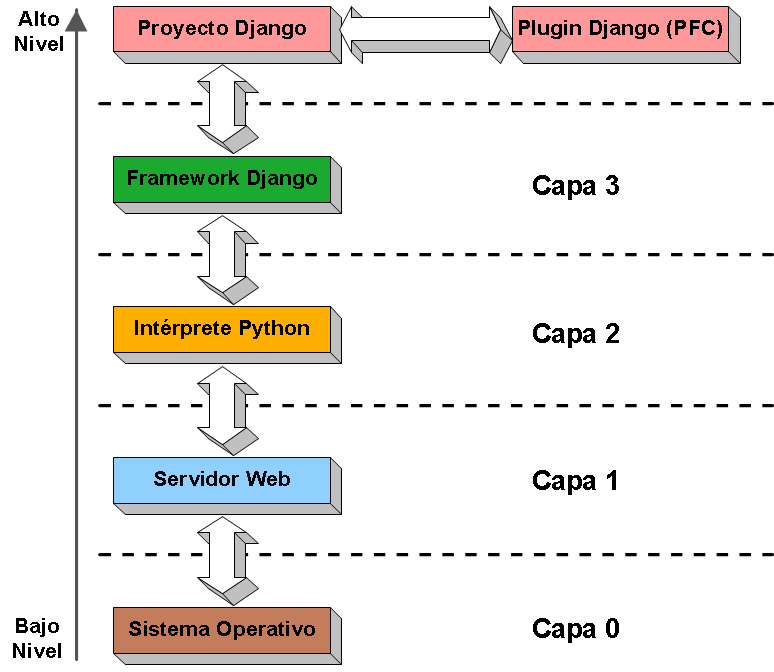
\includegraphics[width=1\textwidth]{disenio/arquitectura_logica.png}
    \end{center}
    \caption{Arquitectura lógica de cada uno de los elementos software}
    \label{fig:ArquitecturaLogica}
\end{figure}

\subsubsection{Estructura del proyecto}

Una vez que hemos visto como es la arquitectura lógica del proyecto, y en cada
una de las capas en las que podríamos definir el mismo, de forma que cada una de
estas interactúen únicamente con aquellas que están inmediatamente por encima o
por debajo de ella misma, toca describir en mayor profundidad la capa situada
más arriba de la jerarquía, la cual se corresponde a la aplicación que vamos a
desarrollar.

Toda aplicación contenida en un proyecto Django, posee una estructura común, de
forma que puedan identificarse cada uno de los elementos que componentes de
forma inmediata. Esta estructura se puede apreciar a modo orientativo, en la
Figura \ref{fig:ArquitecturaLogicaAplicacion}, donde se muestran cada uno de los
componentes principales de una aplicación. A continuación se describen la
finalidad de cada uno de estos apartados:
\begin{itemize}
    \item \textbf{Models:} se trata de un fichero llamado \textit{models.py} o
        un directorio llamado \textit{models}, el cual contendrá diferentes
        ficheros python, en donde se describirán cada uno de los modelos que
        componen a la aplicación Django.
    \item \textbf{Forms:} se trata de un fichero llamado \textit{forms.py} o un
        directorio llamado \textit{forms}, el cual contendrá diferentes ficheros
        python, en donde se describirán cada uno de los diferentes tipos de
        formularios Django.
    \item \textbf{Views:} se trata de un fichero llamado \textit{views.py} o un
        directorio llamado \textit{views}, el cual contendrá diferentes ficheros
        python, donde se describirán cada uno de los modelos que componen a la
        aplicación Django.
    \item \textbf{Templates:} se trata de un directorio común para todo el
        proyecto Django, en el cual se contendrán cada una de las plantillas las
        cuales se usarán por las vistas para mostrar la información en el
        formato especificado en la plantilla.
    \item \textbf{Static:} es un directorio donde se almacenan todos los
        elementos, tanto media, como estilos, javascript, etc\ldots que se
        usará en dicha aplicación.
    \item \textbf{Url's:} es un fichero llamado \textit{urls.py} o un directorio
        llamado \textit{urls}, que contendrá una serie de ficheros python, donde
        se definirán cada una de las URIs de las que dispondrá nuestro proyecto,
        y se asociarán con las vistas que se activará al llamar a dicha URI.
\end{itemize}

Estos componentes que hemos comentado son solo los principales, ya que además de
estos componentes, pueden existir muchos otros para otras finalidades.

\newpage

\begin{figure}[H]
    \begin{center}
        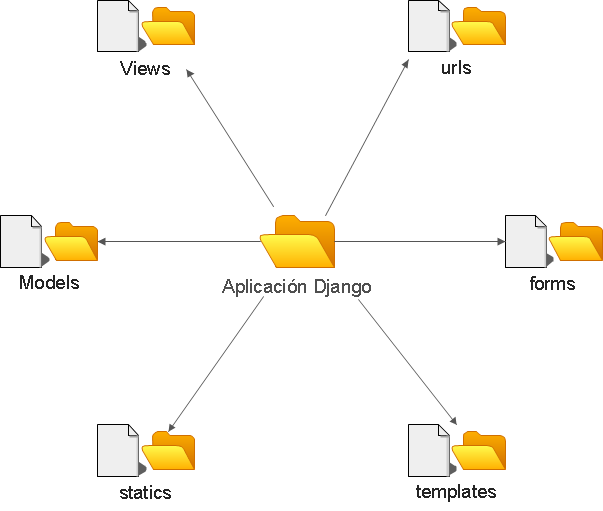
\includegraphics[width=0.95\textwidth]{disenio/arquitectura_logica_aplicacion.png}
    \end{center}
    \caption{Arquitectura lógica de una aplicación Django}
    \label{fig:ArquitecturaLogicaAplicacion}
\end{figure}


\subsection{Arquitectura de diseño}
La arquitectura de diseño especifica la forma en que los artefactos software de
más bajo nivel, interactúan entre sí para lograr el comportamiento deseado en el
sistema. Utilizaremos el patrón arquitectónico  Layers (Capas), con el cual
estructuramos el sistema en un número apropiado de capas, de forma que todos los
componentes de una misma capa trabajan en el mismo nivel de abstracción y los
servicios proporcionados por la capa superior utilizan internamente los
servicios proporcionados por la capa inmediatamente inferior.

Es este caso, para la realización del proyecto, estamos utilizando Django, que
se trata de un framework que aunque no lo sigue fielmente, está basado en el
patrón de diseño MVC (Modelo-Vista-Controlador), de tal forma que en toda
aplicación Django se hace una separación entre los distintos artefactos software,
los cuales interactuando entre sí, conforman el comportamiento esperado del
software. Por consiguiente, tal y como se aprecia en la figura de más abajo
(Figura \ref{fig:DjangoPattern}) podemos decir que toda la lógica de una
aplicación Django se encuentra dividida en los siguientes artefactos:
\begin{itemize}
    \item Los modelos.
    \item Las URL's.
    \item Las views (o vistas).
    \item Los templates (o plantillas).
\end{itemize}

\begin{figure}[H]
    \begin{center}
        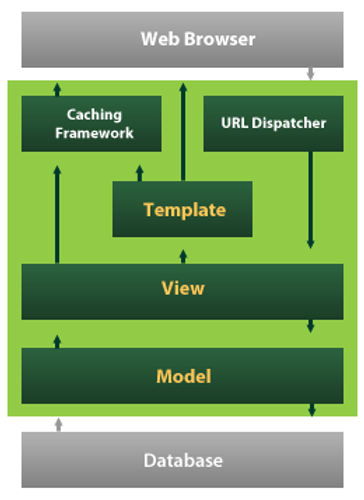
\includegraphics[width=0.6\textwidth]{disenio/esquema_django.png}
    \end{center}
    \caption{Patrón de diseño usado en el framework Django (fuente:
              \href{http://cambioderuta.wordpress.com/2010/01/11/\%C2\%BFque-es-django/}{Cambioderuta})}
    \label{fig:DjangoPattern}
\end{figure}

A continuación, vamos a relacionar cada uno de estos artefactos con la capa con
la que se corresponderían cada uno: presentación, negocio o integración.

\subsubsection{Capa de presentación}
Este grupo de artefactos software conforman la capa de presentación del sistema,
incluyendo tanto los componentes de la vista como los elementos de control de la
misma.

En el framework Django, esta capa se correspondería con los conocidos como
\textit{templates}. Mediante el uso de plantillas en Django, se consigue
separar la presentación de un documento, de la obtención y tratamiento de los
datos. En las plantillas se definen los rellenos y alguna lógica de control
básica para determinar como mostrar los datos. Mediante las plantillas de Django,
aunque el resultado más común pueda ser HTML, se puede generar cualquier tipo de
documento basado en texto, donde presentar los datos.
\subsubsection{Capa de negocio}
Este grupo de artefactos software conforman la capa de negocio del sistema,
incluyendo los elementos del modelo de dominio y los servicios (operaciones del
sistema).

En el caso del framework Django, la capa de negocio estaría fuertemente ligada
con los views (o las vistas, que se corresponden con los controladores en el
patrón MVC). En las vistas de Django, se lleva a cabo el tratamiento de los
datos, se consultan y se realizan operaciones de los mismos, y opcionalmente
estos se envían a la capa de presentación (los templates de Django) donde se
muestran al usuario. Si nos fijamos en la figura \ref{fig:DjangoPattern},
podemos ver, que los controladores hacen un poco como nexo de unión entre los
templates y los modelos (entre la capa de presentación y de integración).
\subsubsection{Capa de integración}
Este grupo de artefactos software conforman la capa de integración del sistema,
incluyendo las clases de abstracción para el acceso a datos (BD o sistema de
ficheros) o a sistemas heredados.

En esta capa, entran en juego diferentes elementos del framework Django.
Primeramente podríamos nombrar a los modelos, estos no son otra cosa, sino
clases Python, las cuales son una representación de las tablas que hay
almacenadas en la base de datos, junto con sus características (restricciones,
valores iniciales, etc), mediante esto se simplifica mucho la representación de
los datos para el usuario, ya que los tratará como objetos de una clase.

Por otro lado, aparecen los managers, estos elementos son una interfaz la cual
poseen todos los modelos de un proyecto Django (son configurables, ya que se
pueden crear interfaces que muestren solo ciertos datos), a través de la cual,
permite al usuario realizar consultas (desde sencillas hasta complejas), usando
un lenguaje propio de consulta del framework (evitamos tener que hacer uso de
SQL, aunque también puede utilizarse este). Con esto, llegamos a la tercera
característica, ya que al hacer uso de un lenguaje propio de consultas en Django,
estas son válidas para cualquier sistema de bases de datos soportado por Django
(este posee distintos backends para distintos motores de bases de datos), de
forma que una misma aplicación funcione con bases de datos PostgreSQL, Oracle,
etc \ldots sin necesidad de realizar cambios en las consultas.
\subsubsection{Servicios transversales}
Este grupo de artefactos software pueden ser usados por elementos de cualquiera
de las capas del sistema y fundamentalmente proporcionan servicios relacionados
con requisitos no funcionales (calidad).

Para nuestro caso, el framework Django posee determinadas características, las
cuales ayudan al cumplimiento de determinados requisitos no funcionales de los
que comentamos anteriormente (Sección \ref{sec:RQNF}), como son los siguientes:
\begin{itemize}
    \item \textbf{Seguridad:} Django incorpora la gestión automática de
        sesiones, o la generación automática de formularios basados el modelos o
        definidos por el programador, incorporando a su vez medidas de seguridad
        (como por ejemplo contra ataques csrf).
    \item \textbf{Mantenibilidad:} la herramienta promueve a la escritura de
        un código fácil de mantener, a parte de estructurar las aplicaciones en
        partes bien diferenciables, de forma que se puedan localizar los
        distintos elementos fácilmente por cualquier desarrollador con algo de
        experiencia en Django, promueve además el uso de patrones de diseño
        (como puede ser el patrón DRY, Facade, etc).
        
        Además, por otro lado, el desarrollo del proyecto, promueve un
        compromiso de seguir unos códigos de buenas maneras definidos en
        \cite{pep8}.
    \item \textbf{Portabilidad:} el framework está desarrollado en Python, el
        cual se trata de un lenguaje multiplataforma, de tal manera que la
        aplicación será válida en cualquier sistema que soporte Python.
\end{itemize}


\section{Diseño de la interfaz de usuario}

En esta sección vamos a proceder a detallar las interfaces que existirán entre
el sistema y el usuario de la aplicación, de forma que se pueda apreciar el
aspecto de estas y el comportamiento que mostrarán las mismas. De forma que sea
más fácil de apreciar para el lector, se van a realizar una serie de bocetos de
cada una de las interfaces, y sobre estos bocetos, se definirá el comportamiento
que tendrán.

Además, a continuación en la figura \ref{fig:mapa_web} se muestra el mapa de
navegabilidad de la aplicación, del cual se realizarán bocetos de las siguientes
interfaces:
\begin{itemize}
    \item Listado de namespaces.
    \item Visibilidad de modelos y atributos.
    \item Visualización de los modelos.
    \item Mapeo de modelos.
    \item Mapeo de los atributos. 
\end{itemize}

\begin{figure}[H]
    \begin{center}
        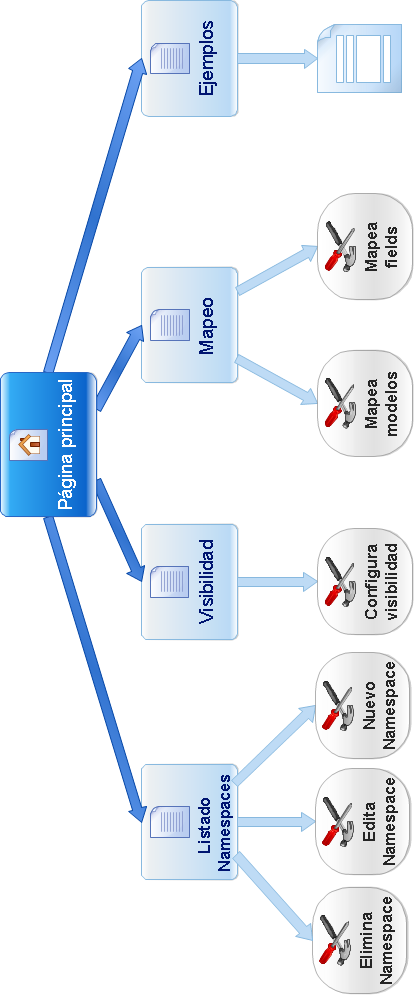
\includegraphics[width=0.45\textwidth]{disenio/mapa_web.png}
    \end{center}
    \caption{Mapa web de la aplicación}
    \label{fig:mapa_web}
\end{figure}

\subsection{Listado de namespaces}

A continuación en la figura \ref{fig:lista_namespaces} se muestra un boceto de
la interfaz para el listado de namespaces de la aplicación.

\begin{figure}[H]
    \begin{center}
        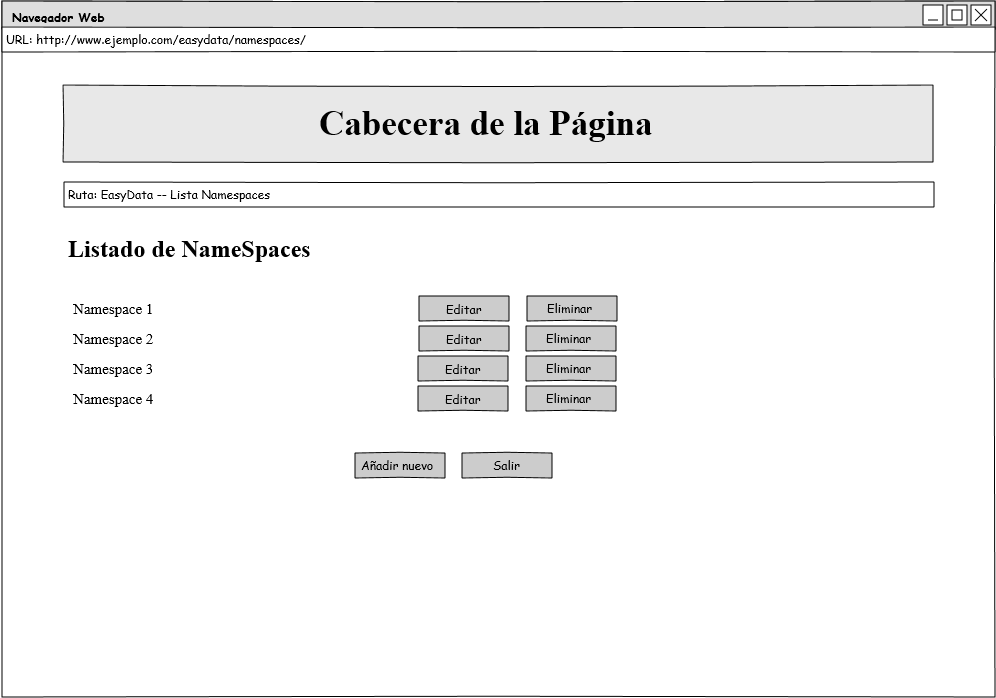
\includegraphics[width=1\textwidth]{mockups/lista_namespaces.png}
    \end{center}
    \caption{Boceto del listado de namespaces}
    \label{fig:lista_namespaces}
\end{figure}

Si observamos el boceto, podemos apreciar que se muestra un listado con cada uno
de los namespaces existentes en la aplicación, los cuales pueden utilizarse para
realizar la exportación de datos. Junto a cada uno de los nampesaces, aparecen
dos botones, los cuales permiten editar las propiedades o actualizar la
especificación de dicho namespace, o eliminar el mismo junto con todas sus
entidades y propiedades.

\subsection{Visibilidad de modelos y atributos}

A continuación en la figura \ref{fig:visibilidad} se muestra un boceto de
la interfaz para la configuración de la visibilidad de los modelos y los
atributos.

\begin{figure}[H]
    \begin{center}
        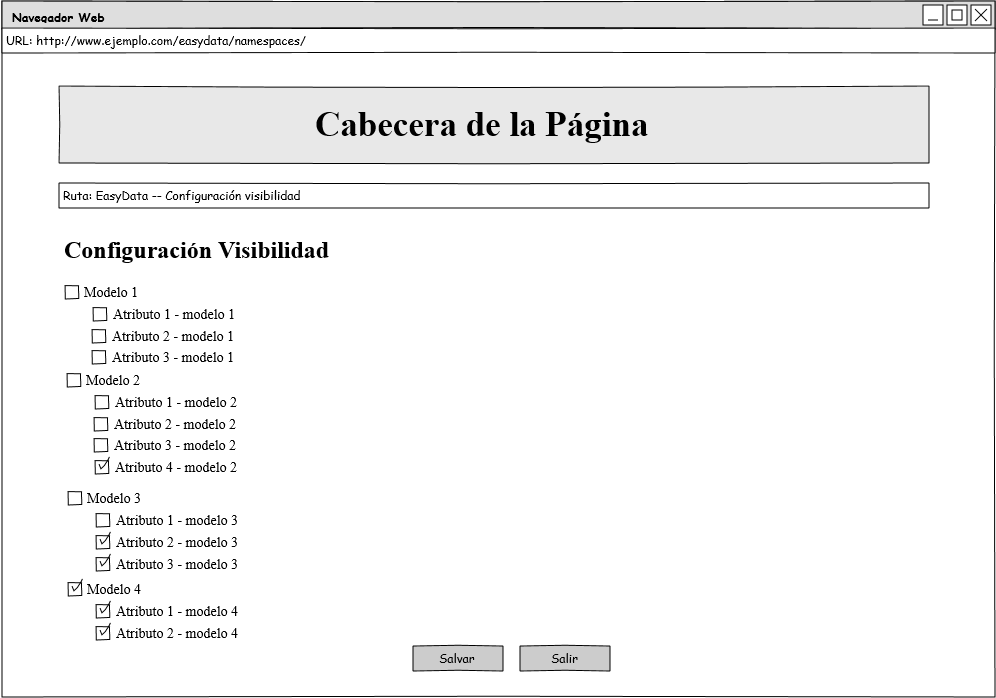
\includegraphics[width=1\textwidth]{mockups/visibilidad.png}
    \end{center}
    \caption{Boceto de la interfaz para la modificación de la visibilidad}
    \label{fig:visibilidad}
\end{figure}

Si observamos el boceto, la configuración de la visibilidad de los modelos y
atributos del proyecto es bastante sencilla. Se muestra al usuario por pantalla
un listado de todos los modelos y atributos que componen a cada uno de estos en
forma de árbol. El usuario marcará aquellos modelos o atributos de estos que
desee que sean visibles. De esta forma, si el usuario quiere que un modelo sea
completamente visible, marcará la casilla del modelo, y además marcará todos los
atributos del mismo. Por otro lado, si un usuario no desea que un determinado
atributo de un determinado modelo no sea visible, únicamente deberá dejar la
casilla correspondiente a dicho modelo sin marcar. Finalmente, si el usuario
desea que un modelo no sea visible, bastará con marcar la casilla
correspondiente al modelo, independientemente de los atributos del mismo que
estén o no marcados.

\subsection{Visualización Modelos}

A continuación en la figura \ref{fig:visualiza_modelos} se muestra un boceto de
la interfaz donde se podrá visualizar la configuración realizada del mapeo de
los diferentes modelos y atributos con los diferentes namespaces cargados en la
aplicación.

\begin{figure}[H]
    \begin{center}
        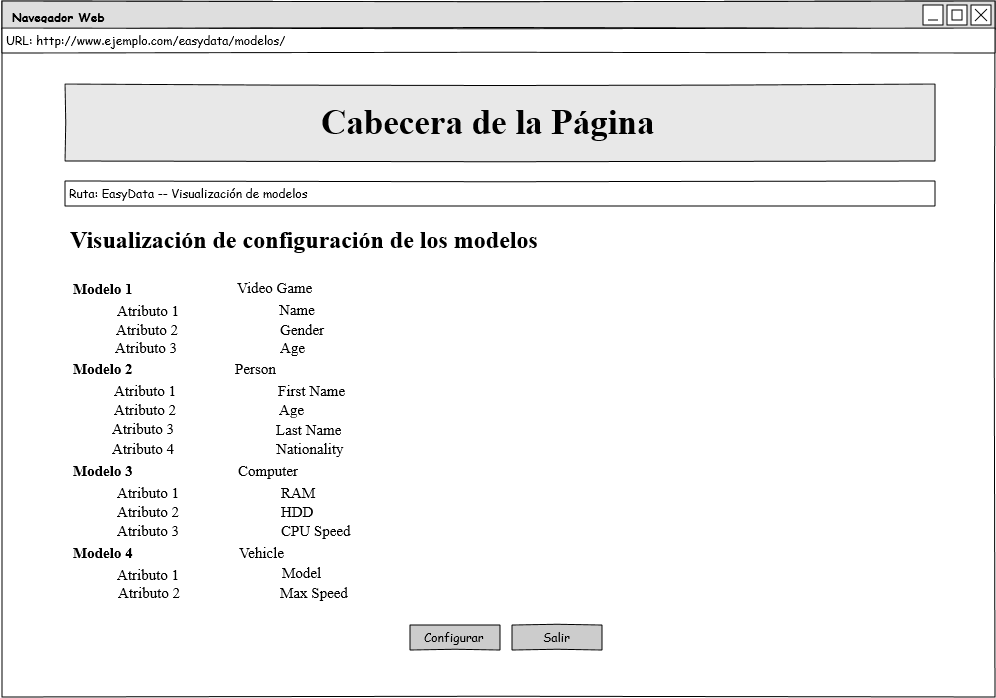
\includegraphics[width=1\textwidth]{mockups/visualiza_modelos.png}
    \end{center}
    \caption{Boceto de la interfaz para visualización del mapeo de los modelos}
    \label{fig:visualiza_modelos}
\end{figure}

Esta pantalla es plenamente informativa, dando al usuario una idea de la
configuración que existe actualmente del mapeo entre los modelos que componen su
proyecto y las entidades de los namespaces. Posteriormente, podrá modificarse la
configuración existente, pulsando sobre el botón \textit{Configurar}.

\subsection{Mapeo de los modelos}

En la figura \ref{fig:mapeo_modelos} de abajo, se muestra un boceto de la
interfaz para la configuración del mapeo de los modelos del proyecto, con las
entidades de los diferentes namespaces que queramos hacer que se corresponda.

\newpage

\begin{figure}[H]
    \begin{center}
        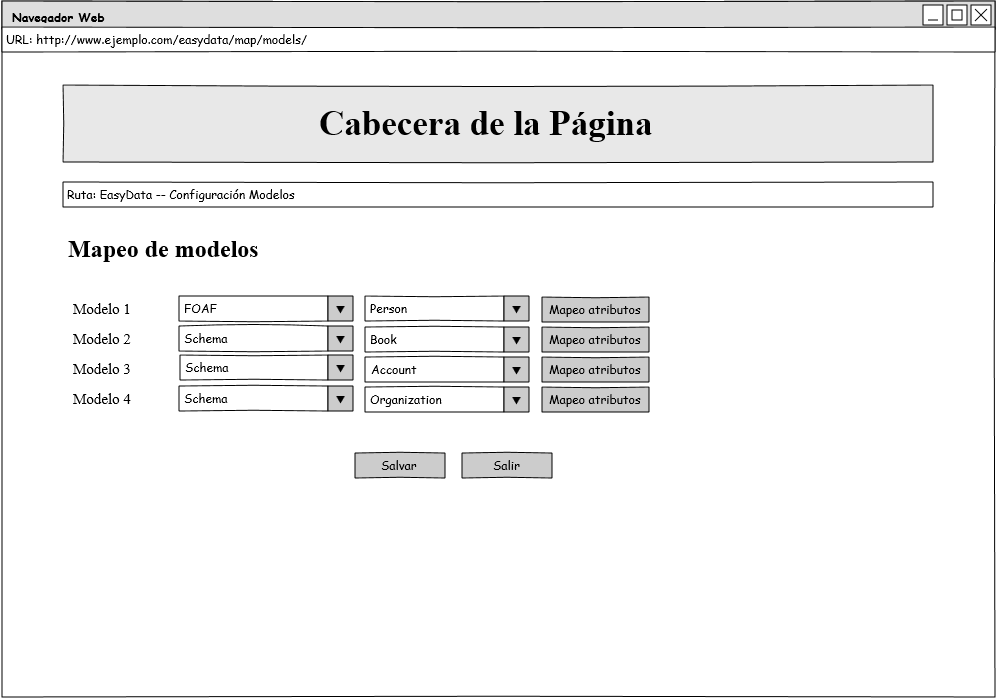
\includegraphics[width=1\textwidth]{mockups/mapeo_modelos.png}
    \end{center}
    \caption{Boceto de la interfaz para el mapeo de los modelos}
    \label{fig:mapeo_modelos}
\end{figure}

El usuario, cuando se encuentre en la pantalla del visualización de la
configuración del mapeo de los modelos, tal y como se indica en el punto
anterior, podrá acceder a configurar dicho mapeo, mostrándole la pantalla
que se puede apreciar, donde para cada uno de los modelos que posee el proyecto
donde se encuentra esta aplicación, mostrará las distintas entidades disponibles
para cada uno de los namespaces. Tras hacer la correspondencia, que el usuario
crea conveniente, solo tendrá que pulsar sobre el botón de salvar, para almacenar
los cambios realizados.

\subsection{Mapeo de los atributos}

En la figura \ref{fig:mapeo_atributos} que se muestra a continuación, podemos
apreciar un boceto de la interfaz que se usará en la aplicación para hacer
corresponder, cada uno de los atributos de los modelos de nuestra aplicación,
con cada posible propiedad de la entidad con la que se ha relacionado el modelo
al que pertenece el atributo, o con cualquiera de las propiedades de los
namespaces cargados.

\begin{figure}[H]
    \begin{center}
        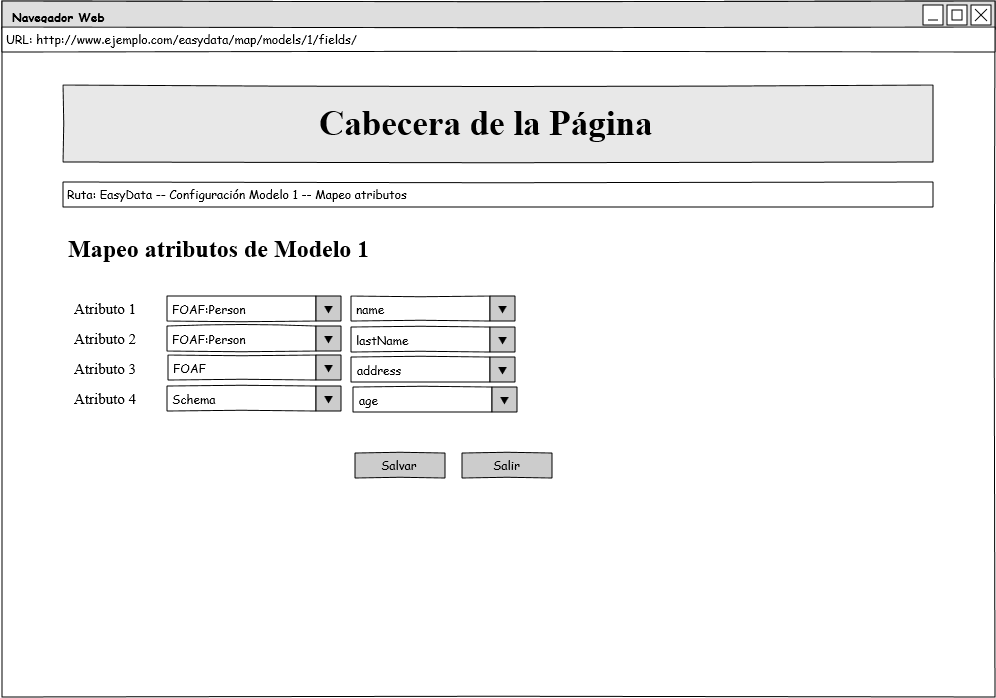
\includegraphics[width=1\textwidth]{mockups/mapeo_atributos.png}
    \end{center}
    \caption{Boceto de la interfaz para el mapeo de los atributos}
    \label{fig:mapeo_atributos}
\end{figure}

Si nos fijamos bien, aparece una entrada por cada uno de los atributos de los
que dispone el modelo, y al lado de cada uno de estos, dos desplegables con cada
uno de los diferentes namespaces y cada una de las posibles propiedades con las
que podremos hacer corresponder al atributo. Una vez se haya realizado toda la
correspondencia, solo habrá que almacenar los cambios realizados pulsando sobre
el botón de salvar.


\section{Diseño de datos}
En esta sección definimos los datos que utilizará la aplicación, y como se
estructuran los mismos dentro de la base de datos. Para plasmar la estructura de
los datos en la base de datos, en la figura \ref{fig:modelo_conceptual} se
muestra el diagrama de datos, donde podemos apreciar cada una de las tablas y
columnas de las mismas existentes en la base de datos, así como las funciones
que implementan cada una de ellas.

\newpage

\begin{figure}[H]
    \begin{center}
        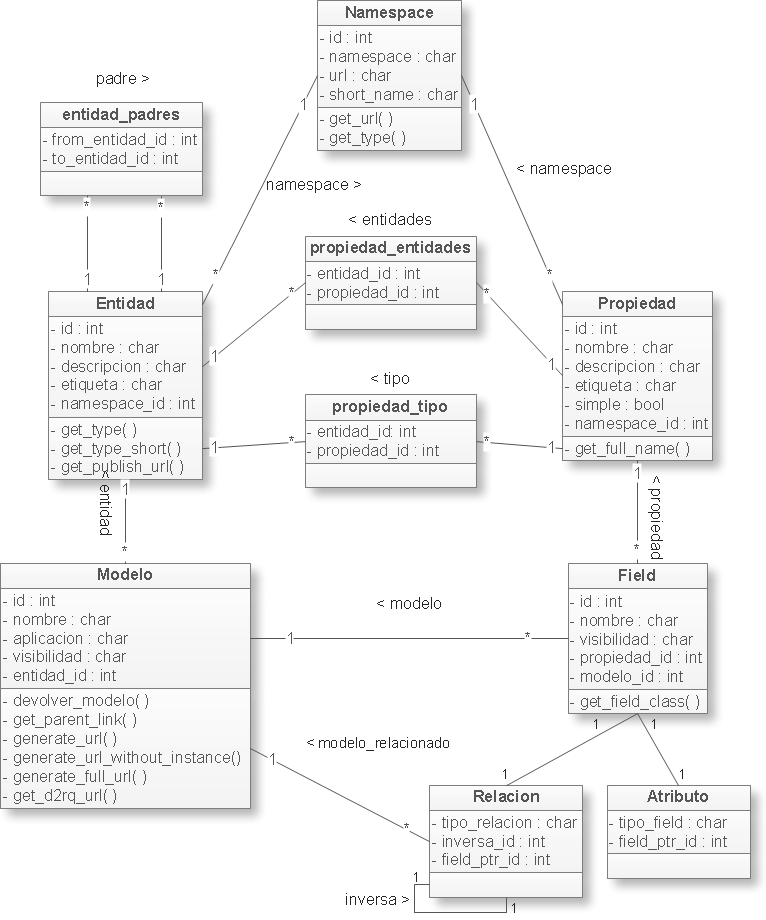
\includegraphics[width=1.0\textwidth]{disenio/modelo_conceptual.png}
    \end{center}
    \caption{Diseño de los datos}
    \label{fig:modelo_conceptual}
\end{figure}

A continuación se detallan cada una de las tablas que aparecen en el diagrama de
diseño de los datos:
\begin{itemize}
    \item \textbf{Namespace:} Esta tabla representa a un determinado namespace,
        almacenando el nombre del mismo y la url donde se encuentra el schema
        que describe cada una de sus entidades y propiedades.
    \item \textbf{Entidad:} Es una determinada entidad de un namespace.
        Almacena el nombre del mismo, y la etiqueta y descripción asociadas en
        el caso de que la posean. Está relacionada con cada una de las
        propiedades que lo componen, con el namespace al que pertenece y con los
        modelos con los que lo haga corresponder el usuario.
    \item \textbf{Propiedad:} Representa a una determinada propiedad de una
        entidad (no tiene que estar relacionado con una entidad forzosamente),
        almacenando el nombre y el tipo de la misma, así como una etiqueta y
        descripción que pueda tener asociados, al igual que en el caso de las
        entidades. Además, estará relacionada con la entidad y el namespace a la
        que pertenece y con los fields con los que lo haya hecho corresponder el
        usuario.
    \item \textbf{Modelo:} Es la representación de cada uno de los modelos de
        los que está compuesto el proyecto Django. Almacena el nombre del mismo,
        la aplicación del proyecto a la que pertenece y la visibilidad que
        tendrá el mismo respecto al exterior. Posee relaciones con la entidad
        con la que se haga corresponder y con los fields de los que está
        compuesto.
    \item \textbf{Field:} Esta tabla a su vez, representa a cada uno de los
        fields del proyecto, que componen a los modelos descritos anteriormente.
        Están compuestos por el nombre de estos y la visibilidad que tendrán
        respecto al exterior. Posee relaciones tanto con el modelo al que
        pertenecen, como con las propiedades con las que se haya hecho
        corresponder. Además, existen dos tablas más, llamadas Atributo y
        Relacion, con una relación OneToOne con la tabla Field (es la forma de
        expresar la herencia en Django), de tal forma que se indica si dicho
        field del modelo es un atributo o una relación.
    \item Las tablas entidad\_padres, propiedad\_entidades y propiedad\_tipo son
        tablas auxiliares que se utilizan para implementar las relaciones
        Muchos-A-Muchos en la base de datos, y los datos que contienen
        únicamente son los punteros (id) a los elementos que relaciona.
\end{itemize}

\section{Diseño de componentes}

En esta sección se definen los componentes software necesarios para la
implementación del sistema. Este sistema se implementa como una única aplicación
Django, pero se puede descomponer en subsistemas en función de las diferentes
funcionalidades que ofrece y de cómo se encontrará estructurado. Al estar
haciendo uso para la realización del proyecto de un framework basado en el
patrón MVC, vamos a diferenciar dentro del mismo, distintos módulos o
componentes, como son los modelos, los controladores y las vistas (conocidos por
modelos, vistas y plantillas respectivamente en Django). En la siguiente figura
(\ref{fig:componentes}) se puede ver un diagrama que refleja perfectamente la
estructura de los componentes que deberá de tener la aplicación.

\newpage

\begin{figure}[H]
    \begin{center}
        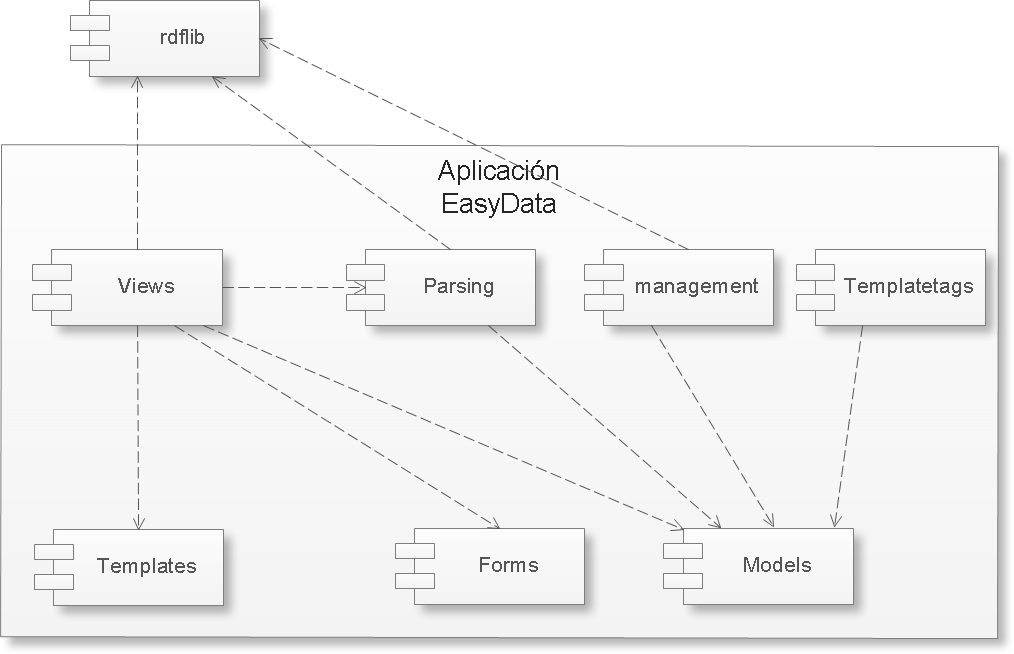
\includegraphics[width=1.05\textwidth]{disenio/modelo_componentes.png}
    \end{center}
    \caption{Estructura de los componentes de la aplicación}
    \label{fig:componentes}
\end{figure}

Donde cada uno de los componentes que se aprecian en la figura
\ref{fig:componentes} son los encargados de realizar las siguientes
funcionalidades:
\begin{itemize}
    \item \textbf{Views:} Almacena todas las vistas de django
        (controladores en el patrón MVC) de los que estará compuesto la
        aplicación, y está dividido en submódulos según la funcionalidad que
        realiza cada uno de la siguiente forma:
    \begin{itemize}
        \item \textbf{map:} almacena aquellas vistas encargadas de realizar el
            mapeo entre los modelos y entidades y entre los fields y
            propiedades.
        \item \textbf{modelo:} almacena las vistas encargadas de configurar la
            visibilidad de los modelos y sus fields.
        \item \textbf{namespaces:} contiene las vistas encargadas de la gestión
            de los namespaces, tanto la alta, edición como eliminado de un
            namespace.
        \item \textbf{publish:} contiene aquellas vistas encargadas de realizar
            la publicación de los datos según el mapeo realizado de los mismos.
        \item \textbf{sesiones:} contiene las vistas encargas de realizar tanto
            el login como el logout de la aplicación.
    \end{itemize}
    \item \textbf{management:} contiene aquellos comandos que se añadirán al
        manage.py de Django. En este caso, se trata de loadmodels y de
        easydata\_d2rq, que se encargará de realizar la captación de los modelos
        y fields del proyecto Django y de generar el fichero de configuración
        para d2rq, respectivamente.
    \item \textbf{Models:} contiene cada uno de los modelos definidos para la
        aplicación EasyData. Cada uno de los módulos de los que está compuesto,
        contiene cada uno de los modelos con el mismo nombre que indica el
        módulo.
    \item \textbf{Template tags:} contiene aquellas funciones que se usarán en
        las plantillas Django para la publicación de información. Está separado
        en dos módulos easydata\_microdata y easydata\_rdfa, para la publicación
        en los formatos en microdata y rdfa respectivamente. Los template tags,
        hacen uso de los modelos para obtener los datos que van a publicar.
    \item \textbf{Parsing:} Contiene aquellas clases y funciones encargadas de
        realizar el parseo de los ficheros RDF (o cualquier otro formato que se
        desee añadir en un futuro) para la carga de nuevos namespaces.
    \item \textbf{Templates:} contiene todas las plantillas donde los
        controladores (vistas de Django), renderizan los datos generados. Estos
        estarán compuestos principalmente por plantillas html.
    \item \textbf{forms:} este componente o módulo de la aplicación contiene
        todos los formularios django que se usarán en las vistas.
    \item \textbf{rdflib:} es un módulo externo que se usará en el proyecto, el
        cuál ofrece funciones para el tratamiento de ficheros RDF.
\end{itemize}

Para plasmar la funcionalidad que tienen cada uno de los componentes que
integran la aplicación, vamos a utilizar diagramas de interacción, donde se
podrá observar como se combinan cada uno de estos para proporcionar una
determinada funcionalidad. Estos elementos no se corresponderán únicamente con
los datos especificados en el diagrama anterior, sino que además podrán verse el
resto de componentes software que intervienen en la prestación de una
determinada funcionalidad. Estas funcionalidades, se corresponderán con aquellas
que hemos descrito en apartados anteriores.

\subsection{Diagramas de interacción}

A continuación mostramos los diagramas de interacción correspondientes a cada
una de las funcionalidades que hemos descrito, las cuales debe de cumplir el
proyecto.
\newpage
\subsubsection{Carga de modelos del proyecto}

\begin{figure}[H]
    \begin{center}
        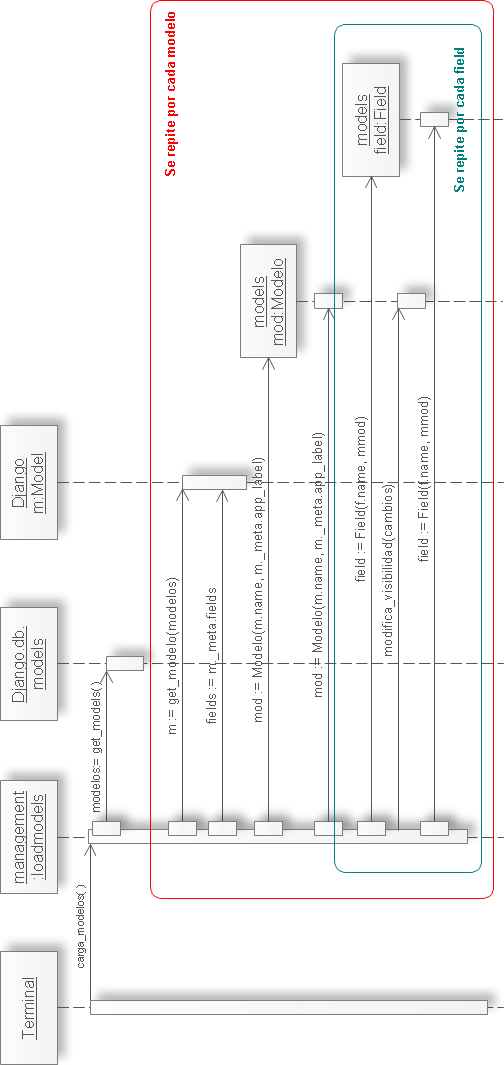
\includegraphics[width=0.62\textwidth]{disenio/interaccion/carga_modelos.png}
    \end{center}
    \caption{Diagrama de interacción: carga de modelos del proyecto}
    \label{fig:carga_modelos}
\end{figure}

\newpage

\subsubsection{Carga de namespaces}

\begin{figure}[H]
    \begin{center}
        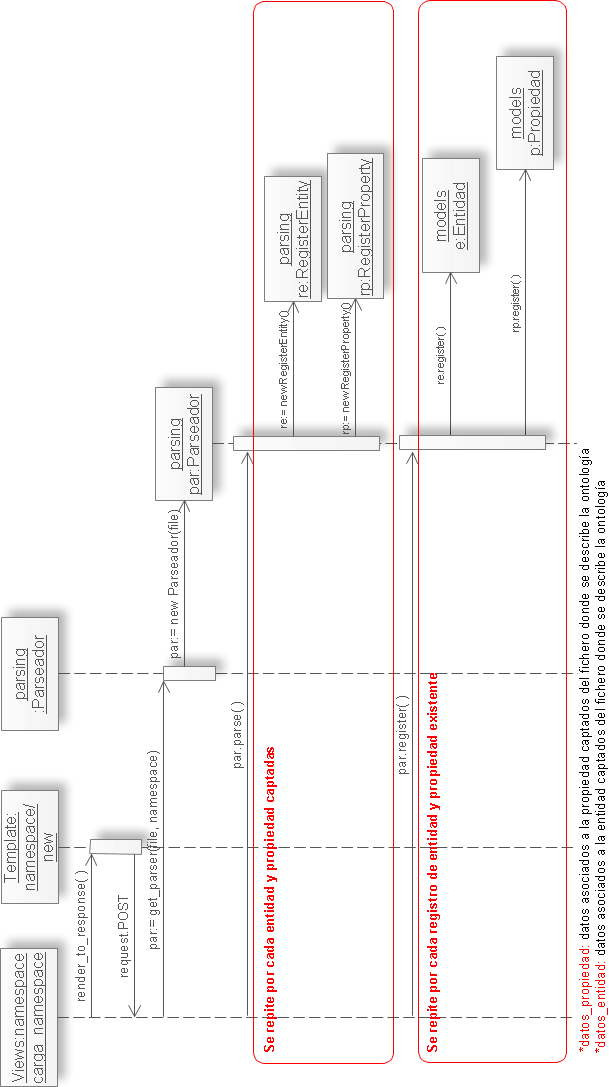
\includegraphics[width=0.65\textwidth]{disenio/interaccion/carga_namespace.png}
    \end{center}
    \caption{Diagrama de interacción: carga de namespaces}
    \label{fig:carga_namespace}
\end{figure}

\newpage

\subsubsection{Configuración de la visibilidad}

\begin{figure}[H]
    \begin{center}
        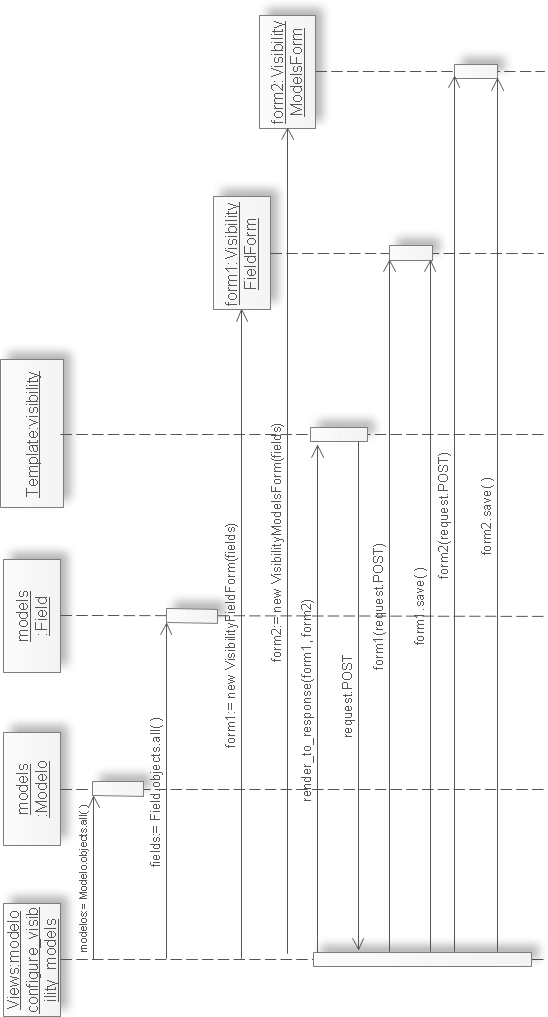
\includegraphics[width=0.7\textwidth]{disenio/interaccion/configurar_visibilidad.png}
    \end{center}
    \caption{Diagrama de interacción: configuración de la visibilidad}
    \label{fig:configura_visibilidad}
\end{figure}

\newpage

\subsubsection{Mapeo de los modelos del proyecto}

\begin{figure}[H]
    \begin{center}
        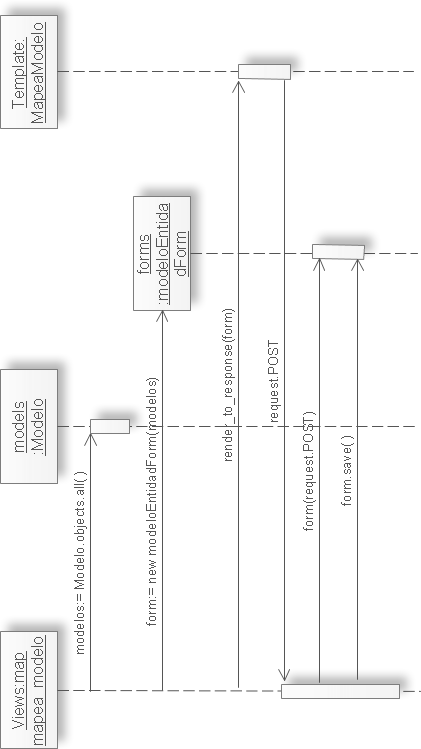
\includegraphics[width=0.7\textwidth]{disenio/interaccion/mapeo_modelos.png}
    \end{center}
    \caption{Diagrama de interacción: mapeo de los modelos del proyecto}
    \label{fig:mapeo_modelos}
\end{figure}

\newpage

\subsubsection{Mapeo de los atributos de los modelos}

\begin{figure}[H]
    \begin{center}
        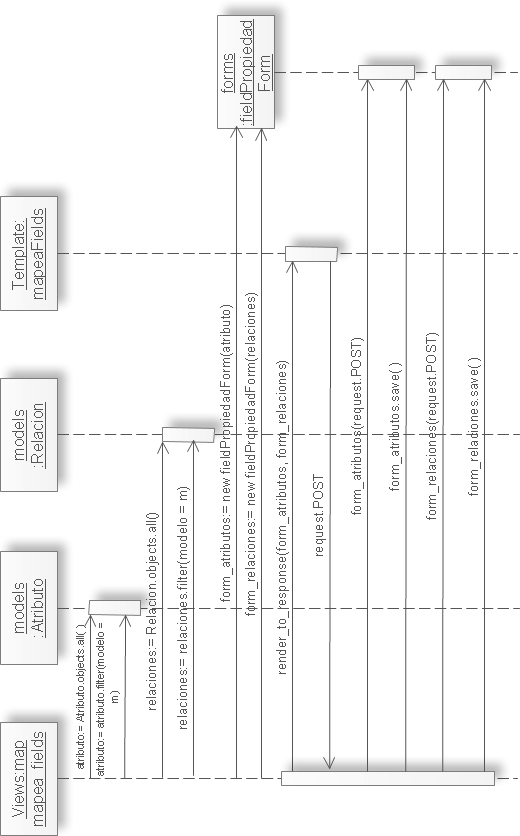
\includegraphics[width=0.7\textwidth]{disenio/interaccion/mapeo_atributos.png}
    \end{center}
    \caption{Diagrama de interacción: mapeo de los atributos de los modelos}
    \label{fig:mapeo_atributos}
\end{figure}

\newpage

\subsubsection{Publicación de datos}

\begin{figure}[H]
    \begin{center}
        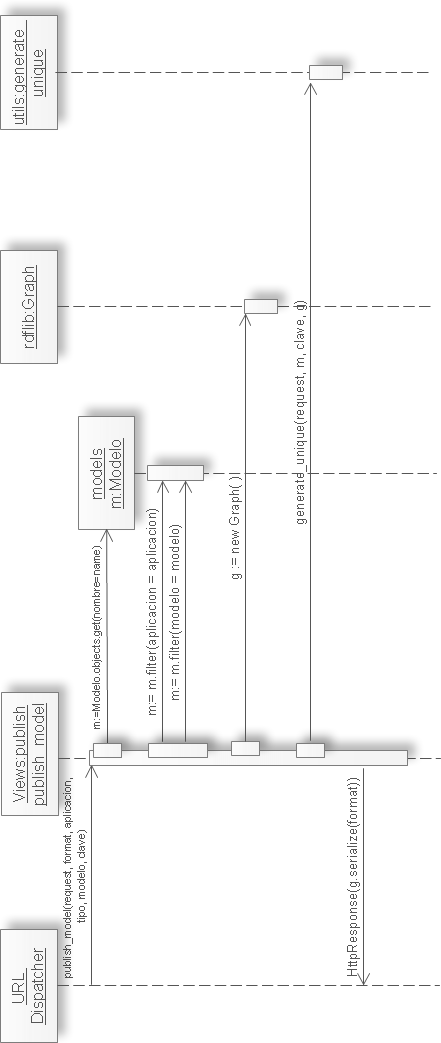
\includegraphics[width=0.58\textwidth]{disenio/interaccion/publicar_datos_element.png}
    \end{center}
    \caption{Diagrama de interacción: publicación de datos para un elemento determinado}
    \label{fig:publicar_datos_element}
\end{figure}

\newpage

\begin{figure}[H]
    \begin{center}
        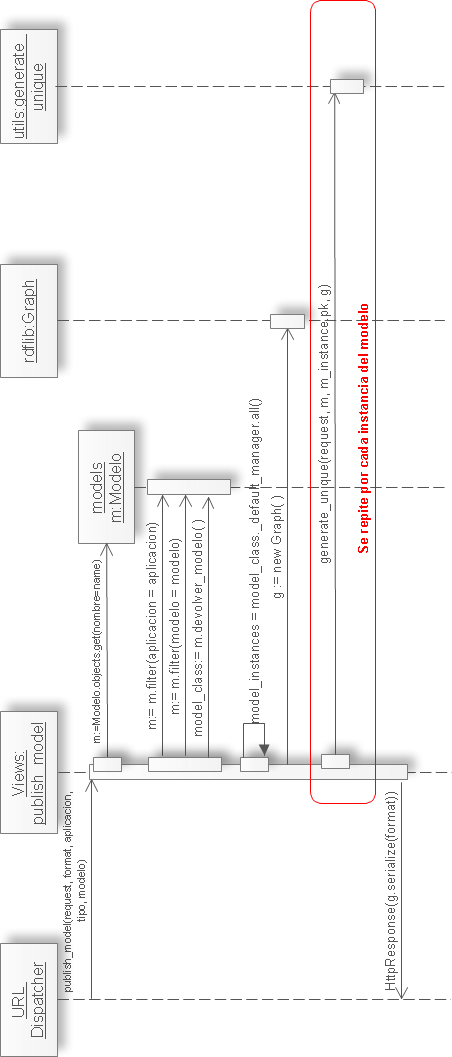
\includegraphics[width=0.6\textwidth]{disenio/interaccion/publicar_datos_model.png}
    \end{center}
    \caption{Diagrama de interacción: publicación de datos para todos los elementos de un modelo}
    \label{fig:publicar_datos_model}
\end{figure}

\newpage

\begin{figure}[H]
    \begin{center}
        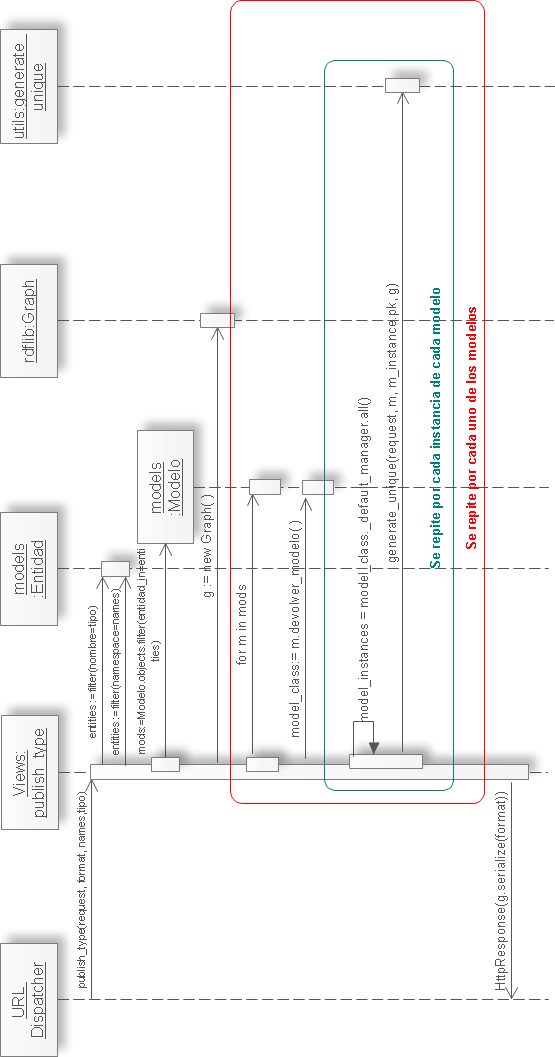
\includegraphics[width=0.7\textwidth]{disenio/interaccion/publicar_datos_type.png}
    \end{center}
    \caption{Diagrama de interacción: publicación de datos para todos los elementos de un tipo}
    \label{fig:publicar_datos_type}
\end{figure}

\newpage

\begin{figure}[H]
    \vspace{4cm}
    \begin{center}
        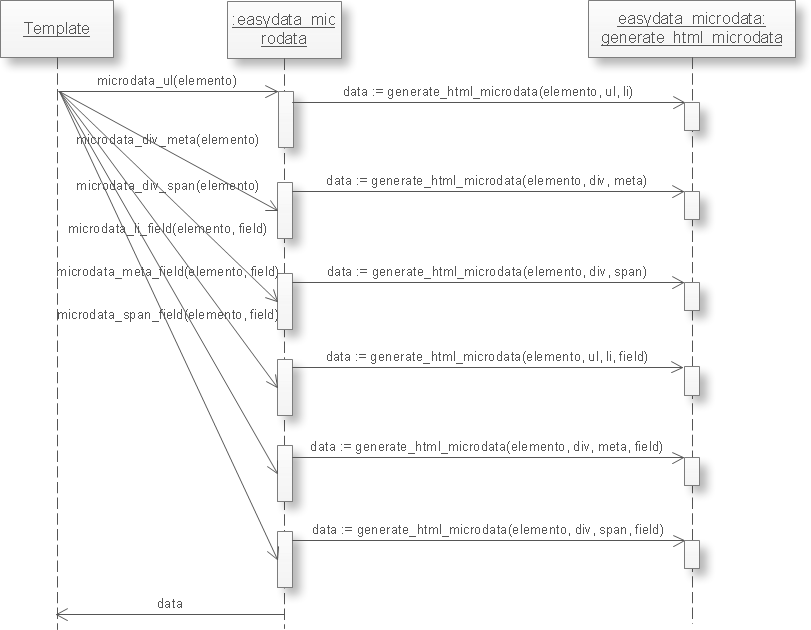
\includegraphics[width=1\textwidth]{disenio/interaccion/publicar_datos_microdata.png}
    \end{center}
    \caption{Diagrama de interacción: publicación de datos mediante microdata}
    \label{fig:publicar_datos_microdata}
\end{figure}

\newpage

\begin{figure}[H]
    \vspace{2cm}
    \begin{center}
        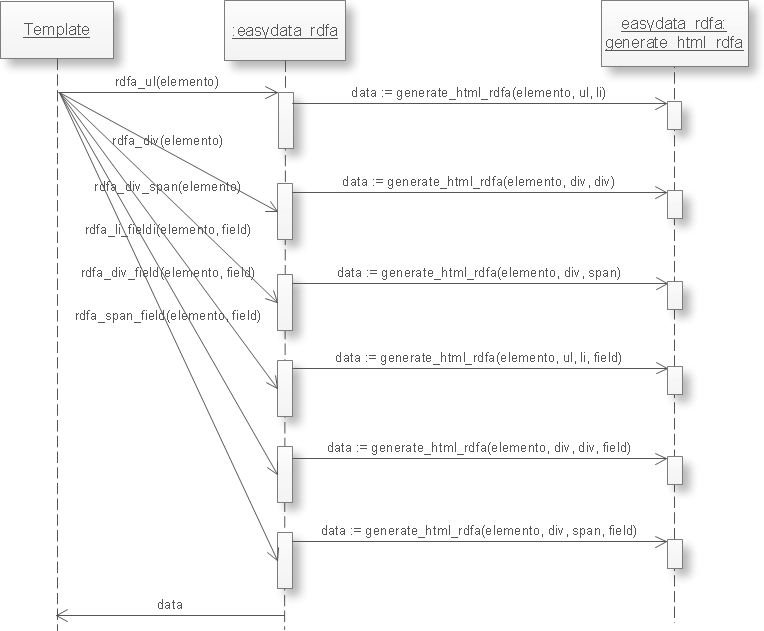
\includegraphics[width=1\textwidth]{disenio/interaccion/publicar_datos_rdfa.png}
    \end{center}
    \caption{Diagrama de interacción: publicación de datos mediante rdfa}
    \label{fig:publicar_datos_rdfa}
\end{figure}

\subsubsection{Generación fichero D2Rq}

\begin{figure}[H]
    \begin{center}
        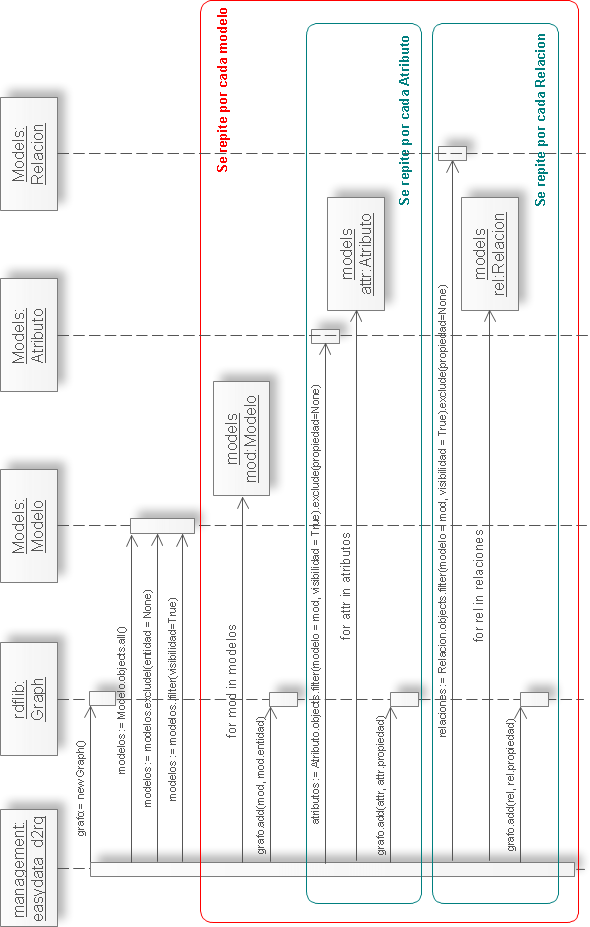
\includegraphics[width=0.8\textwidth]{disenio/interaccion/d2rq.png}
    \end{center}
    \caption{Diagrama de interacción: generación de fichero d2rq}
    \label{fig:d2rq}
\end{figure}

%Para cada uno de los módulos funcionales del sistema debemos realizar un diagrama de secuencia, para definir la interacción existente entre las clases de objetos que permitan responder a eventos externos. A partir de este diagrama, se genera el diagrama de clases de diseño, incluyendo los elementos del modelo conceptual, enriquecidos con las nuevas clases, relaciones, atributos y operaciones resultantes. Asimismo, se detallará el comportamiento de las operaciones más relevantes.


\chapter{Implementación del Sistema}
% ------------------------------------------------------------------------------
% Este fichero es parte de la plantilla LaTeX para la realización de Proyectos
% Final de Grado, protegido bajo los términos de la licencia GFDL.
% Para más información, la licencia completa viene incluida en el
% fichero fdl-1.3.tex

% Copyright (C) 2012 SPI-FM. Universidad de Cádiz
% ------------------------------------------------------------------------------

Este capítulo trata sobre todos los aspectos relacionados con la implementación
del sistema en código, haciendo uso de un determinado entorno tecnológico.

\section{Entorno tecnológico}
En esta sección se indica el marco tecnológico utilizado para la construcción
del sistema, como son:
\begin{itemize}
    \item Entorno de desarrollo (IDE).
    \item Lenguaje de programación, bibliotecas y frameworks de desarrollo
          empleados.
    \item Herramientas de ayuda a la construcción y despliegue.
    \item Control de versiones y repositorio de componentes.
\end{itemize}

El lenguaje de programación utilizado para la elaboración del proyecto ha sido
Python, usándose multitud de bibliotecas de todas las que ofrece el lenguaje,
pero en especial, se ha hecho uso de la biblioteca \textit{rdflib}, la cual ha
permitido tanto el parseo de fichero rdf, como la generación del rdf para la
exportación de datos, en diferentes formatos.

Dentro del lenguaje Python, se ha utilizado el framework \textit{Django}, ya que
el proyecto básicamente consiste en el desarrollo de un plugin para dicho
framework. Además del framework Django, también se ha hecho uso de otros
frameworks, los cuales facilitasen tanto la escritura de estilos CSS como de
código JavaScript. Estos frameworks auxiliares utilizados son \textit{jQuery}
\cite{jQuery} y \textit{Bootstrap} \cite{Bootstrap}.

Tanto en la importación de vocabularios para la aplicación como en la
publicación de los datos, ha sido necesario utilizar formatos específicos, como
son el caso de \textit{RDF/XML}, \textit{RDF/Ntriples}, \textit{RDF/Turtle},
\textit{RDFa} o \textit{Microdata}. Además, en la importación de los datos de
los vocabularios, ha sido necesario utilizar el lenguaje de consultas
\textit{SPARQL}, que permite realizar consultas sobre conjuntos de datos
definidos en ficheros RDF. También se ha hecho uso del software D2Rq, que ofrece
al usuario a partir del esquema de la base de datos, múltiples utilidades para
la publicación de sus datos en internet.

Como IDE de desarrollo, se ha utilizado un editor de texto simple, en este caso
gEdit, con plugins para programación, y el resaltado de código python. A su vez,
también se han utilizado herramientas proporcionadas por la comunidad Python
para la depuración del código, tales como \textit{iPython} y \textit{ipdb}.

Para el despliegue del proyecto se ha utilizado el servidor de pruebas que
ofrece el framework Django, y el servidor \textit{Apache} junto con el
intérprete de apache para código Python \textit{mod\_wsgi}.

Por último, para el alojamiento del código fuente y demás ficheros que componen
el proyecto, se ha hecho uso del sistema de control de versiones
\textit{subversion}, integrado el mismo con la aplicación \textit{Redmine} para
la gestión de tareas y asignaciones de tiempo.

\section{Código fuente}
La organización del código fuente del proyecto, se ha llevado a cabo siguiendo
las indicaciones del propio framework Django para la estructura de sus
aplicaciones, de tal forma que en directorio raíz del proyecto cabría destacar
los siguientes subdirectorios y ficheros:
\begin{itemize}
    \item \textbf{forms:} en este directorio se encuentran alojados todos los
        formularios Django que se utilizan dentro de la aplicación. A su vez,
        este directorio está compuesto por el directorio modelforms, que
        contiene todos los formularios basados en modelos de Django.
    \item \textbf{decorators:} en este directorio se encuentran implementado el
        decorador utilizado en las vistas, para comprobar que el usuario que
        intenta acceder a ellas, se encuentra logueado y tiene permisos de
        superusuario.
    \item \textbf{locale:} en este directorio se encuentran las traducciones de
        la aplicación a los diferentes idiomas que soporta la misma.
        Inicialmente está soportado los idiomas inglés y español.
    \item \textbf{management:} este directorio contiene a su vez el directorio
        commands, el cual contiene todos los comandos desarrollados, a fin de
        que puedan ser ejecutados desde el manage.py de Django desde una
        terminal.
    \item \textbf{models:} este directorio contiene todos los modelos que
        componen a la aplicación Django. Contiene un fichero por cada uno de los
        modelos de la aplicación.
    \item \textbf{parsing:} este directorio no es común a todo proyecto Django,
        pero se encarga de agrupar todas las clases y métodos necesarios para el
        parseo y carga de ontologías en formato RDF.
    \item \textbf{static:} este directorio compuesto a su vez por un
        subdirectorio cuyo nombre es el mismo de la aplicación, se encarga de
        almacenar todos los elementos estáticos de la aplicación, ya sean
        imágenes, estilos, código JavaScript, etc.
    \item \textbf{templates:} este directorio compuesto también a su vez por un
        subdirectorio con el mismo nombre de la aplicación, se encarga de
        almacenar todas las plantillas del proyecto django.
    \item \textbf{templatetags:} este directorio contiene todos los template
        tags desarrollados que pueden ser usados en las plantillas django. Se
        divide en dos ficheros, easydata\_microdata y easydata\_rdfa, y cada
        uno de ellos contienen los template tags necesarios para exportar la
        información en formato microdata y rdfa respectivamente.
    \item \textbf{views:} este directorio contiene todos los ficheros python con
        las vistas que se usarán en la aplicación. Existen varios ficheros, y se
        encargan de agrupar las vistas por funcionalidades comunes.
    \item \textbf{urls.py:} contiene todas las asociaciones de urls con las
        distintas vistas de la aplicación.
    \item \textbf{utils.py:} contiene multitud de funciones auxiliares que se
        utilizan tanto para el mapeo de modelos, como para la exportación de los
        datos en distintos formatos.
\end{itemize}

\subsection{Internacionalización y localización}

A la hora de desarrollar el software EasyData/Django se ha tenido en cuenta que
el mismo pueda ofrecer su contenido en diferentes idiomas en función de los
diferentes usuarios.

Para preparar el software para que este pueda ser traducido a diferentes idiomas
(internacionalización) se han seguido las recomendaciones de Django y se han
hecho uso de las herramientas que proporciona, tanto para la traducción de
cadenas en el código Python como para la traducción de las plantillas. De igual
forma, se ofrecen las traducciones de la aplicación (localización) en los
idiomas inglés y español.

\section{Calidad de código}

Para asegurar la calidad del código fuente y por consiguiente, su fácil
mantenibilidad, además de estructurar la aplicación tal y como recomienda Django,
se ha seguido la guía de estilos para escribir código Python llamada PEP8. La
guía de estilos PEP8 proporciona una serie de convenciones para la codificación
en Python. De esta forma, además de proporcionarme una forma de trabajo y de
escribir un código claro, nos aseguramos en cierta medida, que el código será
fácilmente entendible por cualquier programador que esté acostumbrado a utilizar
esta guía de estilos. A parte del
\href{http://www.python.org/dev/peps/pep-0008/}{manual PEP8} que se encuentra
publicado en la web oficial de Python, existe una herramienta para diferentes
sistemas operativos, con el mismo nombre que la guía de estilos, que comprueba
directamente si nuestro código cumple con las especificaciones de pep8.

Además de la guía de estilos PEP8, también se ha utilizado la herramienta PyLint
que proporciona una métrica que permite obtener una idea de en qué medida el
código de la aplicación es de calidad. Para obtener dicha métrica se basa en
diferentes como puede ser:
\begin{itemize}
    \item Cantidad de comentarios de código (ni poco comentado ni
        sobrecomentado), que no existan elementos como clases, funciones o
        modulos sin comentar.
    \item Que se cumplan patrones de diseño como el patron DRY (Don't repeat
        yourself), de tal forma que no existan abundantes sentencias de código
        repetidas.
    \item Que el proyecto se encuentre correctamente estructurado.
    \item Cumplimiento de convenciones en la escritura del códgio fuente, como
        en el nombre de variables, clases, interlineado, etc\ldots
    \item Que no existan errores en el código.
\end{itemize}

Una vez ejecutada la prueba de calidad de código con PyLint, se ha obtenido una
puntuacion de 9,3 sobre 10 para el código de la aplicación, haciendo uso de un
fichero de configuración de PyLint específico para proyectos Django. Además solo
existe un 1,345\% de líneas duplicadas (89 líneas) de entre mas de 5000 líneas
de código que ha abarcado la aplicación. El resultado es el que se puede
apreciar en la figura \ref{fig:pylint}.

La finalidad de realizar estas pruebas de código, además de que el código
escrito cumpla con un mínimo de calidad, sirve a título personal para la
adquisición de buenas prácticas a la hora de programar, las cuales se puedan
poner en práctica en futuros proyectos.

\begin{figure}[H]
    \begin{center}
        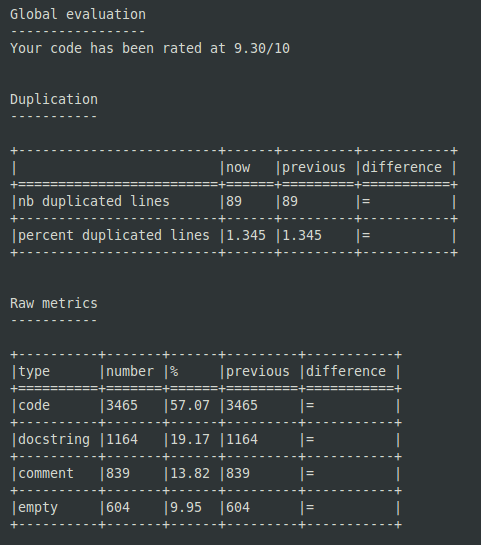
\includegraphics[width=0.6\textwidth]{pruebas/pylint.png}
    \end{center}
    \caption{Resultado de pruebas de validación de PyLint}
    \label{fig:pylint}
\end{figure}


\chapter{Pruebas del Sistema}
% ------------------------------------------------------------------------------
% Este fichero es parte de la plantilla LaTeX para la realización de Proyectos
% Final de Grado, protegido bajo los términos de la licencia GFDL.
% Para más información, la licencia completa viene incluida en el
% fichero fdl-1.3.tex

% Copyright (C) 2012 SPI-FM. Universidad de Cádiz
% ------------------------------------------------------------------------------

En este capítulo se documentan los diferentes tipos de pruebas que se han
llevado a cabo, ya sean de carácter manual o automatizadas mediante software
específico de pruebas.

\section{Pruebas unitarias y de integración}

Para el desarrollo de las pruebas unitarias y de integración de los distintos
artefactos software desarrollados, se han realizado una serie de pruebas
automatizadas mediante el framework de Python para el desarrollo de pruebas
PyUnit, el cual está basado en el framework de pruebas JUnit de Java.

Mediante las pruebas automáticas desarrolladas, se ha probado que tanto los
modelos y métodos de que disponen los mismos realizan las funciones para las que
han sido desarrollados correctamente. Además, también se ha probado la
integración entre los mismos, así como las distintas funciones auxiliares
desarrolladas, donde se combinan el uso de los distintos modelos, así como sus
métodos.

Para lanzar La ejecución de las distintas pruebas automáticas diseñadas, se hará
de la siguiente forma, desde una terminal de escritorio en el directorio donde
se encuentre el fichero manage.py de nuestro proyecto Django:

\begin{lstlisting}[frame=L, language=bash, basicstyle=\footnotesize]
$> python manage.py test easydata
\end{lstlisting}

Esto muestra un informe de los distintos tests ejecutados, así como los posibles
errores que hayan podido surgir en los mismos si alguna de las funciones no se
llevado a cabo tal y como se esperaba. El resultado de la validación debe de ser
similar al que puede apreciarse en la siguiente figura (\ref{fig:pyunit}).

\begin{figure}[H]
    \begin{center}
        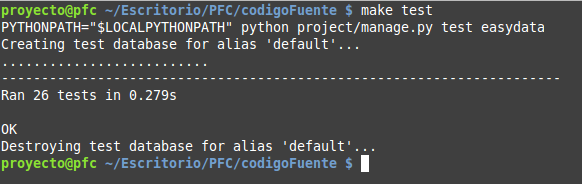
\includegraphics[width=1\textwidth]{pruebas/pyunit.png}
    \end{center}
    \caption{Resultado de validación PyUnit}
    \label{fig:pyunit}
\end{figure}

Adicionalmente, al tratarse de una aplicación la cual se instalará en proyectos
Django ya existentes, se ha probado su integración con aplicaciones disponibles
en el \textit{Python Package Index} desarrolladas por otros autores. Más
concretamente, para el desarrollo de las pruebas que se muestran a continuación,
se ha utilizado la aplicación django-blog-zinnia, que como su nombre indica, se
trata de un blog escrito en Python para Django.

%Las pruebas unitarias tienen por objetivo localizar errores en cada nuevo artefacto software desarrollado, antes que se produzca la integración con el resto de artefactos del sistema. 

%Este tipo de pruebas tienen por objetivo localizar errores en módulos o subsistemas completos, analizando la interacción entre varios artefactos software.


\section{Pruebas de sistema}

En este apartado se describen las pruebas de sistema de modo que se asegure que
el sistema cumple con todos los requisitos establecidos al comienzo del
proyecto, bajo un entorno específico para pruebas.

Para ello se han realizado pruebas manuales, donde se ha comprobado que se
cumplen los requisitos funcionales especificados inicialmente, accediendo a los
distintos apartados de:
\begin{itemize}
    \item \textbf{Captación de modelos y fields del proyecto Django:} se ha
        probado que la carga de modelos y fields del proyecto funciona
        correctamente, así como la actualización de los datos antes posibles
        cambios en los modelos.
    \item \textbf{Carga de nuevos namespaces:} se ha probado que la carga de
        nuevos namespaces u ontologías funciona correctamente, además de la
        actualización de la especificación de los mismos ante posibles cambios.
        Para ello se ha probado con multitud de namespaces diferentes
        suministrados por distintas organizaciones.
    \item \textbf{Configuración de la visibilidad de los modelos y fields:} se
        ha probado que tanto el proceso de configuración de la visibilidad
        funcione correctamente, como que a la hora de publicar los datos,
        aquellos marcados como no visibles no se publiquen a los usuarios
        utilizando las diferentes herramientas de publicación de datos.
    \item \textbf{Mapeo de modelos y fields:} se ha probado que el mapeo de los
        datos funciona correctamente utilizando varios namespaces de forma
        individual o simultánea para un mismo modelo. Posteriormente, se ha
        comprobado que los datos se publican haciendo uso de las etiquetas
        especificadas en este apartado de configuración.
    \item \textbf{Publicación de datos en RDF, RDFa y Microdata:} Una vez
        realizada tanto la carga de modelos y fields, como la configuración de
        los mismos comentada anteriormente, se ha probado que estos se publican
        correctamente según los criterios especificados.
    \item \textbf{Herramienta de generación de D2Rq:} se ha probado que una vez
        realizada la configuración de los modelos y fields, se genera el fichero
        con la configuración para el software D2Rq y este funciona correctamente
        con la aplicación, probando consultas SPARQL y comprobando que los
        resultados sean satisfactorios.
    \item \textbf{Generación de diagrama con configuración:} una vez realizada
        la configuración de los modelos y los fields, se ha probado que la
        generación del diagrama con la configuración mediante Graphviz, se
        corresponde con la configuración realizada.
\end{itemize}

Además de la comprobación de que se han satisfacido cada uno de los requisitos
funcionales descritos en el apartado de análisis del proyecto, se han realizado
pruebas de validación, de los datos exportados.

A continuación se muestra un resumen de las pruebas de validación realizadas
sobre los datos publicados por la aplicación EasyData/Django.

\subsection{Pruebas no funcionales} 

\subsubsection{Pruebas de validación de RDF}

La validación del código RDF generado por la aplicación EasyData/Django, se ha
hecho uso del validador suministrado por el W3C
(\url{http://www.w3.org/RDF/Validator/}). Para la realización de la prueba, se
suministró al validador del W3C diferentes salidas proporcionadas por la
aplicación EasyData/Django, comprobando en cada caso que el resultado de la
validación fuese satisfactorio. De esta forma, obtenemos la seguridad de que los
datos RDF publicados, están perfectamente generados y cumple estrictamente los
estándares impuestos por el W3C.

A continuación, se muestra un ejemplo de una salida generada por la aplicación
EasyData/Django en formato RDF/XML, para una entrada de blog de la aplicación
anteriormente comentada, donde se pueden apreciar las marcas que se han añadido
en función del mapeo realizado.

\begin{lstlisting}[frame=L, language=bash, basicstyle=\footnotesize, breaklines=true, numbers=left]
<?xml version="1.0" encoding="UTF-8"?>
<rdf:RDF
   xmlns:foaf="http://xmlns.com/foaf/0.1/"
   xmlns:rdf="http://www.w3.org/1999/02/22-rdf-syntax-ns#"
   xmlns:schema="http://schema.org/"
>
  <rdf:Description rdf:about="http://pfc-llerena.rhcloud.com/easydata/publish/instance/zinnia/BlogPosting-Entry/2.xml">
    <schema:sameAs>Esta es la segunda entrada del blog de zinnia.Ten mucha suerte en tu Proyecto Fin de Carrera.</schema:sameAs>
    <schema:dateModified rdf:datatype="http://www.w3.org/2001/XMLSchema#dateTime">2013-12-01T11:36:17.142964</schema:dateModified>
    <foaf:skypeID rdf:datatype="http://www.w3.org/2001/XMLSchema#integer">2</foaf:skypeID>
    <schema:text>&lt;p&gt;Esta es la segunda entrada del blog de zinnia.&lt;/p&gt;&lt;p&gt;Ten mucha suerte en tu Proyecto Fin de Carrera.&lt;/p&gt;</schema:text>
    <schema:description rdf:datatype="http://www.w3.org/2001/XMLSchema#boolean">false</schema:description>
    <schema:keywords></schema:keywords>
    <foaf:myersBriggs>None</foaf:myersBriggs>
    <rdf:type rdf:resource="http://schema.org/BlogPosting"/>
    <schema:dateCreated rdf:datatype="http://www.w3.org/2001/XMLSchema#dateTime">2013-12-01T11:35:33</schema:dateCreated>
    <schema:datePublished rdf:datatype="http://www.w3.org/2001/XMLSchema#dateTime">2013-12-01T11:36:11</schema:datePublished>
    <schema:headline>Segunda entrada</schema:headline>
    <foaf:page>entry_detail.html</foaf:page>
    <schema:sameAs>segunda-entrada</schema:sameAs>
    <schema:award rdf:datatype="http://www.w3.org/2001/XMLSchema#integer">0</schema:award>
    <schema:about rdf:resource="http://pfc-llerena.rhcloud.com/easydata/publish/instance/zinnia/BlogPosting-Entry/1.xml"/>
  </rdf:Description>
</rdf:RDF>
\end{lstlisting}

En la figura \ref{fig:rdftest} se puede apreciar una captura de pantalla con el
resultado de la validación devuelto por el validador del W3C, donde se puede
ver que el código RDF cumple con los estándares impuestos por el W3C.

\newpage

\begin{figure}[H]
    \begin{center}
        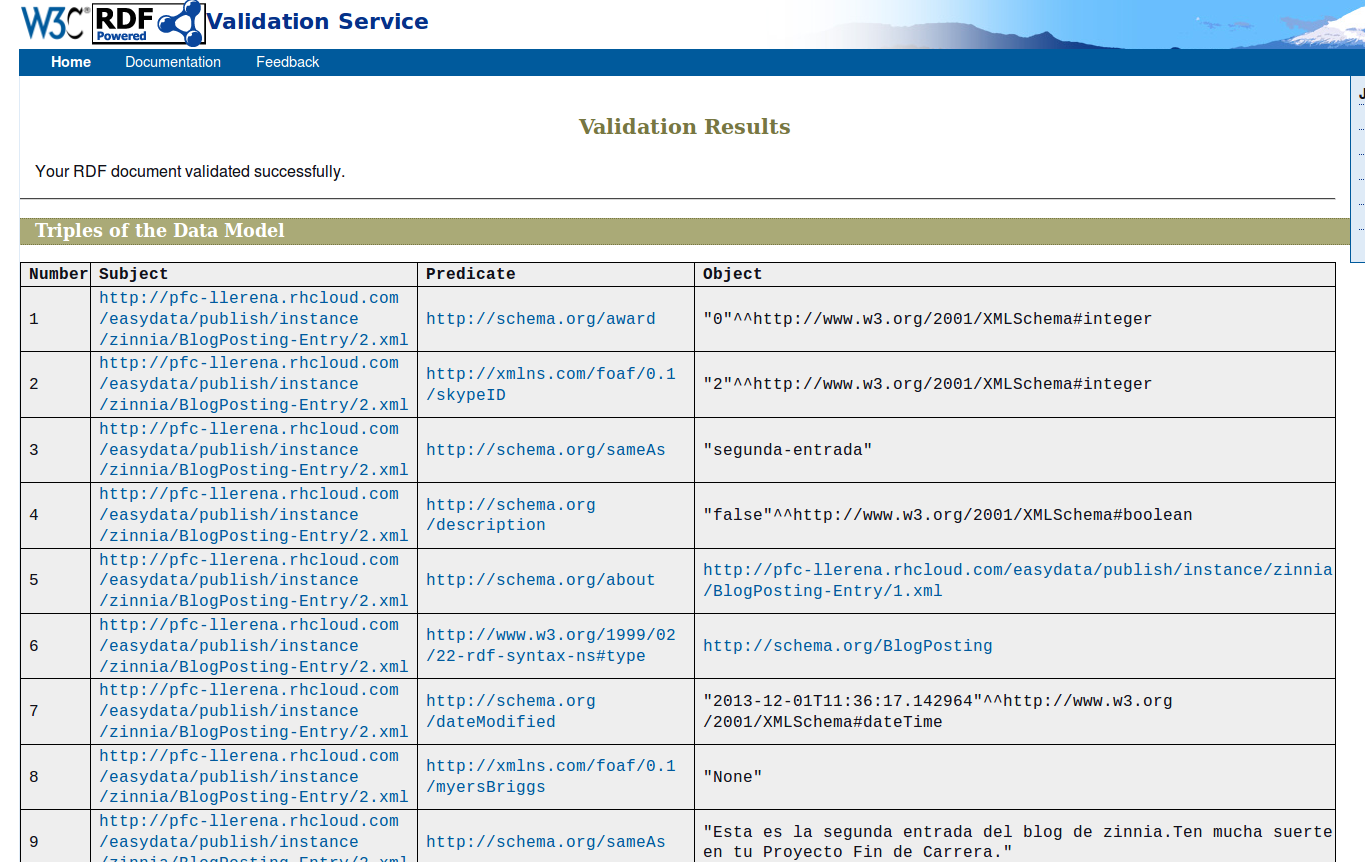
\includegraphics[width=1\textwidth]{pruebas/rdftest.png}
    \end{center}
    \caption{Resultado de validación RDF}
    \label{fig:rdftest}
\end{figure}


\subsubsection{Pruebas de validación de RDFa}

Al igual que para el caso de RDF, también se ha realizado una validación del
código RDFa generado por la aplicación EasyData/Django, haciendo uso de igual
forma del validador suministrado por el W3C
(\url{http://www.w3.org/2012/pyRdfa/Validator.html}). Para la realización de las
pruebas, se suministró al validador del W3C diferentes salidas proporcionadas
por la aplicación EasyData/Django, comprobando en cada caso que el resultado de
la validación fuese satisfactorio. Así de esta forma, nos aseguramos también que
el código RDFa generado por la aplicación, están perfectamente generado y cumple
de igual forma estrictamente los estándares impuestos por el W3C.

A continuación, se muestra un ejemplo de una salida generada por la aplicación
EasyData/Django en formato RDFa, para una entrada de blog de la aplicación
anteriormente comentada, donde se pueden apreciar las marcas que se han añadido
en función del mapeo realizado al lenguaje HTML utilizando la notación RDFa.

\begin{lstlisting}[frame=L, language=HTML, basicstyle=\footnotesize, breaklines=true, numbers=left]
<div about="http://pfc-llerena.rhcloud.com/easydata/publish/instance/zinnia/BlogPosting-Entry/2.xml" typeof="schema:BlogPosting" prefix="schema: http://schema.org/ foaf: http://xmlns.com/foaf/0.1/">
    <div content="2" property="foaf:skypeID"></div>
    <div content="Segunda entrada" property="schema:headline"></div>
    <div content="segunda-entrada" property="schema:sameAs"></div>
    <div content="2013-12-01 11:36:11" property="schema:datePublished"></div>
    <div content="None" property="foaf:myersBriggs"></div>
    <div content="2013-12-01 11:35:33" property="schema:dateCreated"></div>
    <div content="2013-12-01 11:36:17.142964" property="schema:dateModified"></div>
    <div content="&lt;p&gt;Esta es la segunda entrada del blog de zinnia.&lt;/p&gt;&lt;p&gt;Ten mucha suerte en tu Proyecto Fin de Carrera.&lt;/p&gt;" property="schema:text"></div>
    <div content="0" property="schema:award"></div>
    <div content="Esta es la segunda entrada del blog de zinnia.Ten mucha suerte en tu Proyecto Fin de Carrera." property="schema:sameAs"></div>
    <div content="" property="schema:keywords"></div>
    <div content="False" property="schema:description"></div>
    <div content="entry_detail.html" property="foaf:page"></div>
    <link resource="http://pfc-llerena.rhcloud.com/easydata/publish/instance/zinnia/BlogPosting-Entry/1.xml" rel="schema:about">
</div>

<div about="http://pfc-llerena.rhcloud.com/easydata/publish/instance/zinnia/BlogPosting-Entry/1.xml" typeof="schema:BlogPosting" prefix="schema: http://schema.org/ foaf: http://xmlns.com/foaf/0.1/">
    <div content="1" property="foaf:skypeID"></div>
    <div content="Saludo inicial" property="schema:headline"></div>
    <div content="saludo-inicial" property="schema:sameAs"></div>
    <div content="2013-12-01 11:01:17" property="schema:datePublished"></div>
    <div content="None" property="foaf:myersBriggs"></div>
    <div content="2013-12-01 11:00:40" property="schema:dateCreated"></div>
    <div content="2013-12-01 11:01:36.367237" property="schema:dateModified"></div>
    <div content="&lt;p&gt;Esto es una entrada de prueba para el blog de zinnia para probar junto con EasyData.&lt;/p&gt;" property="schema:text"></div>
    <div content="0" property="schema:award"></div>
    <div content="Esto es una entrada de prueba para el blog de zinnia para probar junto con EasyData." property="schema:sameAs"></div>
    <div content="easydata" property="schema:keywords"></div>
    <div content="False" property="schema:description"></div>
    <div content="entry_detail.html" property="foaf:page"></div>
    <link resource="http://pfc-llerena.rhcloud.com/easydata/publish/instance/zinnia/BlogPosting-Entry/2.xml" rel="schema:about">
</div>
\end{lstlisting}

En la figura \ref{fig:rdfatest} se puede apreciar una captura de pantalla con el
resultado de la validación producido por el validador del W3C, donde se puede
ver que el código RDFa cumple con los estándares impuestos por el W3C.

\newpage

\begin{figure}[H]
    \begin{center}
        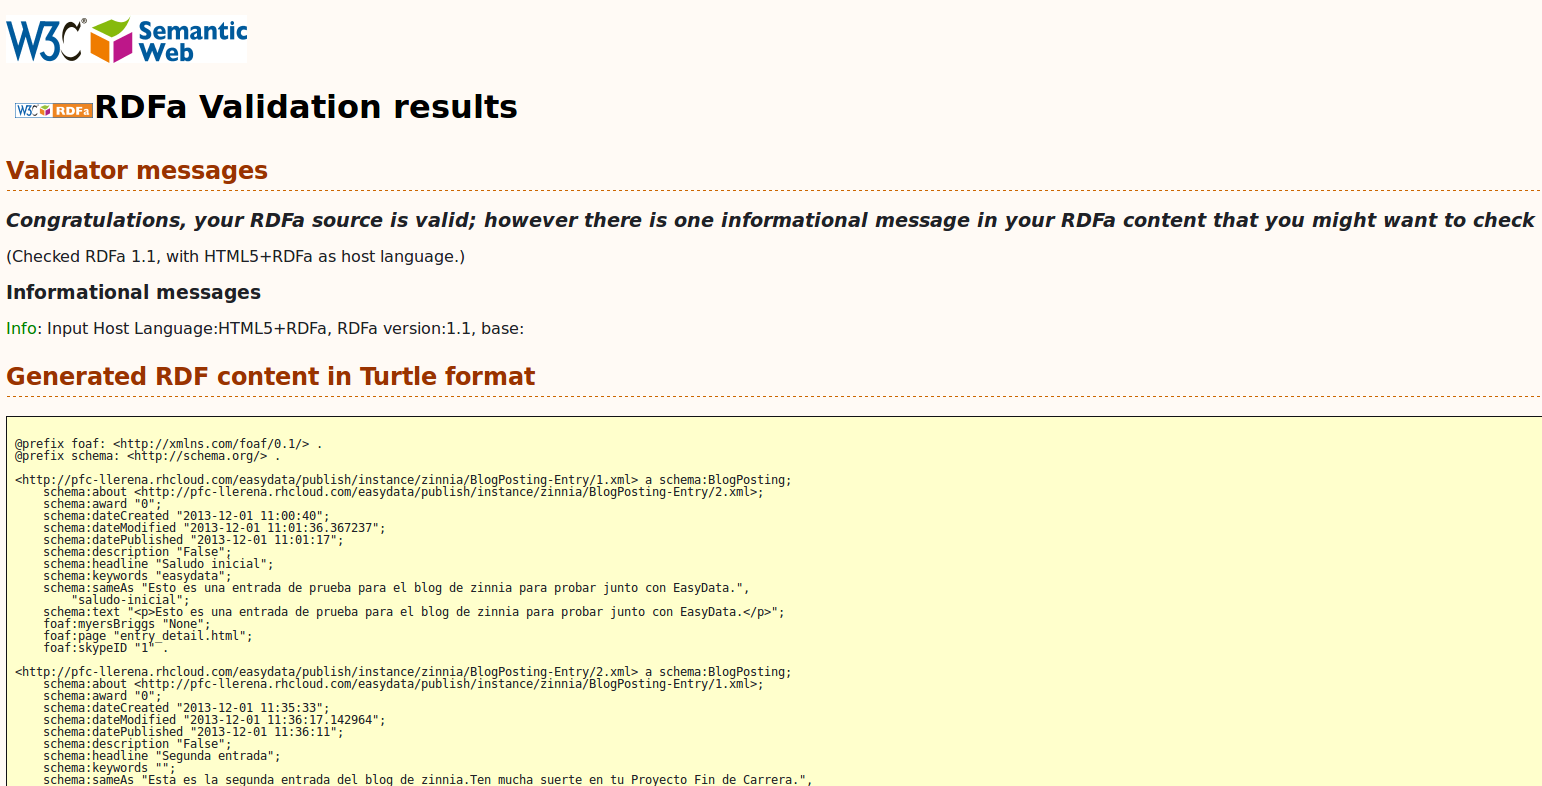
\includegraphics[width=1\textwidth]{pruebas/rdfatest.png}
    \end{center}
    \caption{Resultado de validación RDFa}
    \label{fig:rdfatest}
\end{figure}


\subsubsection{Pruebas de validación de Microdata}

Por último, al igual que en los casos anteriores, también se ha realizado una
validación del código Microdata generado por la aplicación EasyData/Django,
haciendo uso de una herramienta suministrada por Google
(\url{http://www.google.com/webmasters/tools/richsnippets}), la cual busca
metadatos en una determinada URI que se le suministre. Para la realización de la
prueba, se suministró a la herramienta de Google diferentes salidas
proporcionadas por la aplicación EasyData/Django, comprobando en cada caso que
los datos captados por la herramienta fuesen los correctos. Así de esta forma,
nos aseguramos también que el código Microdata generado por la aplicación, está
correctamente construido.

A continuación, se muestra un ejemplo de una salida generada por la aplicación
EasyData/Django en formato Microdata, para una entrada de blog de la aplicación
anteriormente comentada, donde se pueden apreciar las marcas que se han añadido
en función del mapeo realizado al lenguaje HTML utilizando la notación Microdata.

\begin{lstlisting}[frame=L, language=HTML, basicstyle=\footnotesize, breaklines=true, numbers=left]
<div itemid="http://pfc-llerena.rhcloud.com/easydata/publish/instance/zinnia/BlogPosting-Entry/2.xml" itemtype="http://schema.org/BlogPosting" itemscope >
    <span itemprop="http://xmlns.com/foaf/0.1/skypeID">2</span>
    <span itemprop="http://schema.org/headline">Segunda entrada</span>
    <span itemprop="http://schema.org/sameAs">segunda-entrada</span>
    <span itemprop="http://schema.org/datePublished">2013-12-01 11:36:11</span>
    <span itemprop="http://xmlns.com/foaf/0.1/myersBriggs">None</span>
    <span itemprop="http://schema.org/dateCreated">2013-12-01 11:35:33</span>
    <span itemprop="http://schema.org/dateModified">2013-12-01 11:36:17.142964</span>
    <span itemprop="http://schema.org/text"><p>Esta es la segunda entrada del blog de zinnia.</p><p>Ten mucha suerte en tu Proyecto Fin de Carrera.</p></span>
    <span itemprop="http://schema.org/award">0</span>
    <span itemprop="http://schema.org/sameAs">Esta es la segunda entrada del blog de zinnia.Ten mucha suerte en tu Proyecto Fin de Carrera.</span>
    <span itemprop="http://schema.org/keywords"></span>
    <span itemprop="http://schema.org/description">False</span>
    <span itemprop="http://xmlns.com/foaf/0.1/page">entry_detail.html</span>
    <link href="http://pfc-llerena.rhcloud.com/easydata/publish/instance/zinnia/BlogPosting-Entry/1.xml" itemprop="http://schema.org/about">
</div>

<div itemid="http://pfc-llerena.rhcloud.com/easydata/publish/instance/zinnia/BlogPosting-Entry/1.xml" itemtype="http://schema.org/BlogPosting" itemscope >
    <span itemprop="http://xmlns.com/foaf/0.1/skypeID">1</span>
    <span itemprop="http://schema.org/headline">Saludo inicial</span>
    <span itemprop="http://schema.org/sameAs">saludo-inicial</span>
    <span itemprop="http://schema.org/datePublished">2013-12-01 11:01:17</span>
    <span itemprop="http://xmlns.com/foaf/0.1/myersBriggs">None</span>
    <span itemprop="http://schema.org/dateCreated">2013-12-01 11:00:40</span>
    <span itemprop="http://schema.org/dateModified">2013-12-01 11:01:36.367237</span>
    <span itemprop="http://schema.org/text"><p>Esto es una entrada de prueba para el blog de zinnia para probar junto con EasyData.</p></span>
    <span itemprop="http://schema.org/award">0</span>
    <span itemprop="http://schema.org/sameAs">Esto es una entrada de prueba para el blog de zinnia para probar junto con EasyData.</span>
    <span itemprop="http://schema.org/keywords">easydata</span>
    <span itemprop="http://schema.org/description">False</span>
    <span itemprop="http://xmlns.com/foaf/0.1/page">entry_detail.html</span>
    <link href="http://pfc-llerena.rhcloud.com/easydata/publish/instance/zinnia/BlogPosting-Entry/2.xml" itemprop="http://schema.org/about">
</div>
\end{lstlisting}

En la figura \ref{fig:microdatatest} se puede apreciar una captura de pantalla
con el resultado de la validación producido por el validador de Google, donde se
puede ver que que se extraen correctamente los datos del código Microdata.

\newpage

\begin{figure}[H]
    \begin{center}
        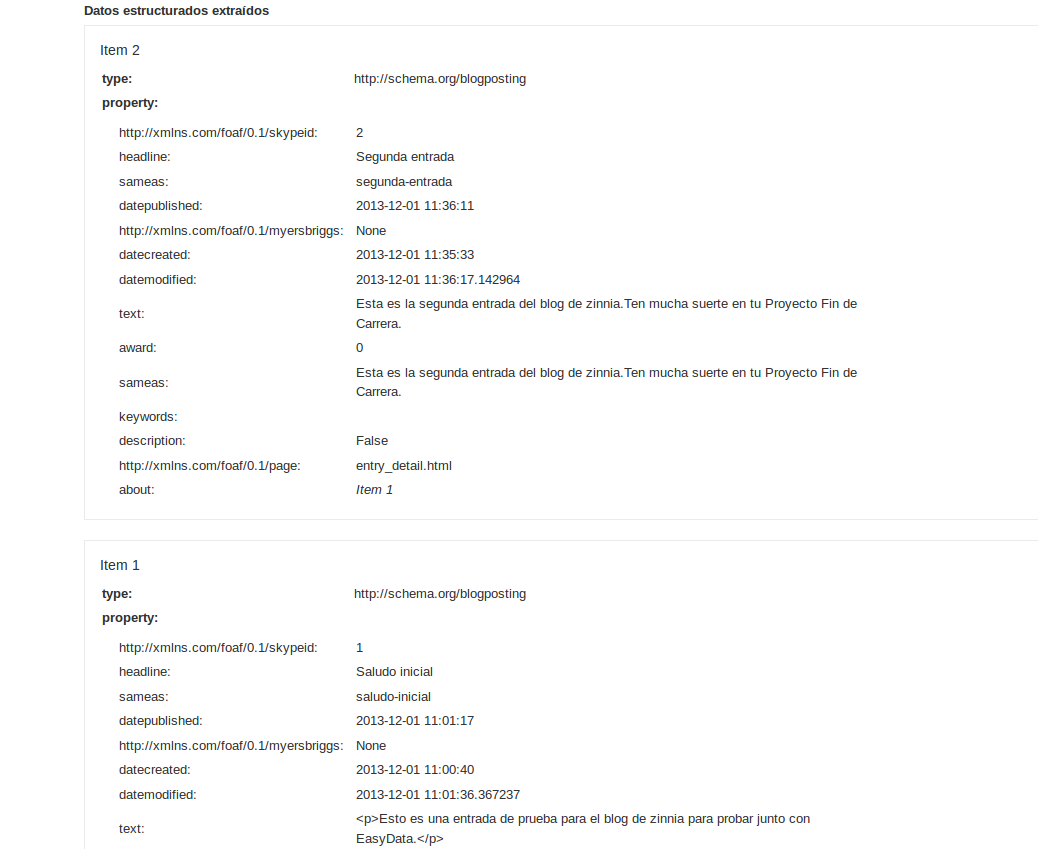
\includegraphics[width=1\textwidth]{pruebas/microdatatest.png}
    \end{center}
    \caption{Resultado de validación Microdata}
    \label{fig:microdatatest}
\end{figure}

\subsubsection{Resto de pruebas no funcionales}

Por otro lado, para llevar a cabo el resto de pruebas no funcionales, se ha
realizado una validación manual, asegurándonos de que se cumplen el resto de
requisitos no funcionales impuestos para la aplicación, como son:
\begin{itemize}
    \item \textbf{Seguridad:} comprobando que las vistas son únicamente
        accesibles para usuarios administradores de Django, y que únicamente se
        publican aquellos datos que el usuario ha marcado como visibles.
    \item \textbf{Portabilidad:} habiéndose usado siempre herramientas
        compatibles con python, o soportadas por múltiples plataformas.
    \item \textbf{Entorno tecnológico:} se ha desarrollado una aplicación
        perfectamente compatible con las versiones iguales o superiores a Django
        1.4.
    \item \textbf{Mantenibilidad:} se trata de una aplicación desarrollada como
        un paquete python, el cual cumple con las reglas impuestas por el PEP8
        para la escritura de código y habiéndose realizado una evaluación de la
        calidad del código fuente con la herramienta PyLint.
\end{itemize}

% Estas pruebas pretenden comprobar el funcionamiento del sistema, con respecto a los requisitos no funcionales definidos en la etapa de análisis: rendimiento, accesibilidad, etc. 

% \section{Pruebas de aceptación}
% El objetivo de estas pruebas es demostrar que el producto está listo para el paso a producción. Suelen ser las mismas pruebas que se realizaron anteriormente pero en el entorno de producción. En estas pruebas, es importante la participación del cliente final.


% EPILOGO
\part{Epílogo}
%\null\vfill
%\noindent En esta última parte quedarán recogidas las conclusiones y los manuales necesarios para el manejo de la aplicación resultado del desarrollo. Si se ha realizado algún tipo de evaluación de la solución proporcionada, más allá de las pruebas del sistema, también deberá venir recogida en un capítulo separado dentro de esta parte. Pueden consultarse diversos tipos de evaluaciones sobre sistemas de información en \cite{hevner2004}: casos de estudio, análisis estático, análisis dinámico, simulación, experimento controlado, etc.
%\vfill

\chapter{Manual de instalación y explotación}
\label{chap:maninsexp}
% ------------------------------------------------------------------------------
% Este fichero es parte de la plantilla LaTeX para la realización de Proyectos
% Final de Grado, protegido bajo los términos de la licencia GFDL.
% Para más información, la licencia completa viene incluida en el
% fichero fdl-1.3.tex

% Copyright (C) 2012 SPI-FM. Universidad de Cádiz
% ------------------------------------------------------------------------------

A continuación, se detallan la instrucciones para la correcta instalación y
explotación de la aplicación EasyData/Django para la apertura de datos en
proyectos Django.

% Las instrucciones de instalación y explotación del sistema se detallan a
% continuación.

\section{Introducción}

El software EasyData/Django, ofrecerá al usuario que incorpore la aplicación a
su proyecto facilidades a la hora de la publicación de los datos de su base de
datos, pudiendo elegir únicamente aquellos que estime conveniente el usuario,
haciendo uso de las diferentes ontologías disponibles en internet (como pueden
ser, Schema, FOAF, etc.), y en diferentes formatos ampliamente utilizados (como
pueden ser RDF, RDFa o microdata).

De esta forma, las principales funcionalidades que ofrece el software al usuario
son las siguientes:
\begin{itemize}
    \item Captación de los distintos modelos y fields de los mismos, de los que
        se encuentra compuesto el proyecto Django donde se instale la aplicación
        EasyData/Django.
    \item Carga de diferentes namespaces en formato RDF disponibles en internet.
    \item Configuración de los datos que serán visibles y aquellos que no se
        considerarán privados y no se mostrarán al exterior.
    \item Correspondencia de los modelos y fields del proyecto con los distintos
        elementos de las ontologías que se hayan cargado en el proyecto.
    \item Publicación de los datos en los diferentes formatos disponibles.
\end{itemize}

\section{Requisitos previos}

Para el correcto funcionamiento de la aplicación EasyData/Django, los únicos
requisitos hardware existentes son los propios de cualquier aplicación Python y
proyecto Django.

Por otro lado, en referencia a los requisitos software, como requisito base será
necesario un sistema operativo el cual permita le ejecución de código Python y
que cumpla con los requisitos software para la ejecución proyectos Django.
Además, como requisitos específicos existen los siguientes:
\begin{itemize}
    \item Al tratarse de una aplicación para proyectos Django, será necesario
        que el proyecto donde se vaya a incluir la aplicación EasyData/Django
        funcione bajo una versión igual o superior a la 1.4 de Django.
    \item Así mismo, también será necesario que se encuentre instalado el
        paquete \textit{rdflib} de Python (a ser posible en su versión 4.0.1, ya
        que no se ha probado para versiones anteriores y no se puede asegurar su
        correcto funcionamiento), ya que esta aplicación hace uso de él para
        ofrecer la mayoría de sus funcionalidades descritas anteriormente.
    \item Además, para la generación de los gráficos mediante Graphviz de la
        configuración de los modelos del proyecto, será necesario el paquete
        pydot.
\end{itemize}

\section{Inventario de componentes}

Junto con la aplicación EasyData/Django se incluyen los siguientes paquetes
software necesarios para el correcto funcionamiento de la aplicación:
\begin{itemize}
    \item Framework jQuery en su versión 1.9.1.
    \item Plugin jQuery-UI para el framework jQuery en su versión 1.10.3.
    \item Framework CSS Bootstrap en su versión 3.0.0.
\end{itemize}


\section{Procedimientos de instalación}
\label{sec:procinsta}

A continuación se detallan cada uno de los pasos necesarios para la correcta
instalación y explotación de la aplicación EasyData/Django dentro de un proyecto
Django.

Lo primero que hay que hacer es instalar los paquetes necesarios para que la
aplicación EasyData/Django funcione dentro de nuestro sistema, por lo que
deberemos de instalar/actualizar la versión de Django de nuestro sistema a una
versión igual o superior a la 1.4 y asegurarnos que nuestro proyecto Django es
compatible con esta versión. Lo primero podemos hacerlo mediante el comando pip:

\begin{lstlisting}[frame=L, language=bash, basicstyle=\footnotesize]
$> pip install django>=1.4
\end{lstlisting}

O bien, entrando en la web oficial de Django y descargando los ficheros fuente
del repositorio de Django y siguiendo las instrucciones de instalación. Esto se
encuentra correctamente explicado en la
\href{https://www.djangoproject.com/download/}{documentación oficial} de Django.

Para la instalación del paquete rdflib de Python, podremos proceder exactamente
de la misma forma, instalando el mismo desde pip de la siguiente forma:

\begin{lstlisting}[frame=L, language=bash, basicstyle=\footnotesize]
$> pip install rdflib==4.0.1
\end{lstlisting}

O bien desde el repositorio oficial GIT del proyecto, el cual se puede encontrar
en \href{https://github.com/RDFLib/rdflib}{GitHub} disponible para su descarga y
perfectamente documentado.

De igual forma, para la instalación del paquete pydot de Python, podemos hacerlo
a través de la herramienta pip de la siguiente forma:

\begin{lstlisting}[frame=L, language=bash, basicstyle=\footnotesize]
$> pip install pydot
\end{lstlisting}

Para la instalación de los paquetes comentados anteriormente, también podemos
hacer uso de la herramienta easy\_install, la cual es bastante similar a pip, de
la siguiente forma:

\begin{lstlisting}[frame=L, language=bash, basicstyle=\footnotesize]
$> easy_install django
$> easy_install rdflib
$> easy_install pydot
\end{lstlisting}

Una vez hemos instalado los paquetes necesarios para la ejecución de la
aplicación EasyData/Django, únicamente nos faltará descargar la aplicación
EasyData/Django y copiar el contenido de la aplicación dentro de nuestro
\textit{PYTHONPATH} o dentro del propio directorio del proyecto Django, junto
con el resto de aplicaciones que componen a dicho proyecto Django.

También existe la posibilidad de descargar la aplicación EasyData/Django desde
el Python Package Index, como hemos hecho con las aplicaciones anteriores de las
que hace uso el proyecto. Además, la aplicación EasyData/Django tiene
especificados los requisitos necesarios para su ejecución, por lo que al
instalarla desde el pip, el propio instalador se encargará de instalar las
aplicaciones de las que depende, ahorrándonos los pasos anteriores. Para ello
procederemos de igual forma que en los casos anteriores introduciendo uno de los
siguientes comandos:

\begin{lstlisting}[frame=L, language=bash, basicstyle=\footnotesize]
$> easy_install django-easydata
\end{lstlisting}

\begin{lstlisting}[frame=L, language=bash, basicstyle=\footnotesize]
$> pip install django-easydata
\end{lstlisting}

Una vez tengamos la aplicación EasyData/Django, el siguiente paso será incluir
dicha aplicación dentro del proyecto Django donde queremos hacer uso de la
misma. Para ello, solo tendremos que añadir la aplicación en el settings.py de
nuestro proyecto dentro de la variable \mbox{INSTALLED\_APPS}, quedando de la
siguiente forma:

\begin{lstlisting}[frame=L, language=Python, basicstyle=\footnotesize]
INSTALLED_APPS = (
    'django.contrib.auth',
    'django.contrib.contenttypes',
    'django.contrib.sessions',
    'django.contrib.sites',
    'django.contrib.messages',
    'django.contrib.staticfiles',
    'django.contrib.admin',
    'easydata',
)
\end{lstlisting}

Cuando hayamos incluido la aplicación \textit{EasyData/Django} en nuestro
proyecto Django, lo siguiente que deberemos hacer será sincronizar la base de
datos, ya que la aplicación \textit{EasyData/Django} hace uso de sus propias
tablas para almacenar la información respecto a los namespaces, modelos y fields
existentes. Para ello, como debería de hacerse con cualquier aplicación,
deberemos ejecutar el siguiente comando en el directorio donde se encuentre el
manage.py de nuestro proyecto:

\begin{lstlisting}[frame=L, language=bash, basicstyle=\footnotesize]
$> python manage.py syncdb
\end{lstlisting}
 
El siguiente paso de la instalación de la aplicación EasyData/Django en nuestro
proyecto Django, será añadir las urls propias de la aplicación a las urls de
nuestro proyecto, de forma que el proyecto pueda servir dichas urls. Para
realizar esto, añada la siguiente línea al fichero url.py de su proyecto:

\begin{lstlisting}[frame=L, language=Python, basicstyle=\footnotesize]
url(r'^easydata/', include('easydata.urls'))
\end{lstlisting}

El nombre asignado de easydata para la url es opcional, de tal forma que se
puede modificar por otro que se adecue mejor a las necesidades del usuario.

Como último paso, la aplicación EasyData/Django usa staticfiles para servir los
ficheros estáticos de la aplicación, por lo que en nuestro proyecto deberá de
estar soportado. Para cargar los ficheros estáticos de la aplicación en nuestro
proyecto, se debe de lanzar el siguiente comando desde nuestro directorio del
proyecto:

\begin{lstlisting}[frame=L, language=bash, basicstyle=\footnotesize]
python manage.py collectstatic
\end{lstlisting}

Para más información acerca de los ficheros estáticos y de cómo se sirven estos
en un proyecto Django, visite la
\href{https://docs.djangoproject.com/en/dev/howto/static-files/}{documentación oficial}.

Por último, se informa al usuario que la aplicación EasyData/Django hace uso del
sistema de usuarios y de roles de Django para el control de permisos a las
vistas de configuración de la publicación de datos, restringiendo el acceso a
todo aquel usuario que no posea los permisos de super usuario de Django. Por lo
que si desea crear un usuario superusuario de Django, deberá hacerlo mediante el
siguiente comando en la terminal:

\begin{lstlisting}[frame=L, language=bash, basicstyle=\footnotesize]
python manage.py createsuperuser
\end{lstlisting}

El asistente se encargará de solicitarle los datos necesarios para la creación
del usuario. Si por otro lado, desea poder utilizar un usuario existente que no
está marcado como superusuario, únicamente deberá marcar a True los campos
\textit{is\_staff} y \textit{is\_superuser}.

\subsection{Otras configuraciones}

Con los pasos explicados anteriormente sería suficiente para que la aplicación
pudiera funcionar correctamente, pero existen otros parámetros de configuración
que pueden modificarse, para personalizar la misma a las necesidades del usuario.

\subsubsection{Cabecera de URLs}
\label{sec:cabeceraurl}

La aplicación EasyData utiliza el framework Sites de Django para obtener la
cabecera de las URLs (dominio), pero si el usuario lo desea, puede especificar
una función alternativa para calcular las cabeceras. Para ello, deberá
implementar una función propia que devuelva una cadena de texto con la cabecera
de las URLs, bajo el nombre \textit{url\_header} y especificar en el settings de
Django el módulo donde se encuentra dicha función mediante la variable
\mbox{\textit{EASYDATA\_URL\_HEADER}}, de manera que EasyData sepa donde buscar
dicha función.

\subsubsection{URIs de modelos}

Por otro lado, la aplicación EasyData de Django, genera una URI única para cada
una de las instancias de los modelos del proyecto Django donde ha sido
instalado, la cual hace referencia a el fichero RDF con los datos de dicha
instancia con el mapeo configurado.

En vez de usar la URI que hace referencia al fichero RDF con los datos de la
instancia, al usuario le podría interesar que se utilizase otro tipo de URI para
identificar a las instancias de un determinado modelo (como por ejemplo la URL
donde de la web donde se lista la información de dicha instancia), por lo que
existe la posibilidad de que el usuario especifique la URL para un determinado
modelo implementando el método \textit{easydata\_generate\_url}, el cual
devolverá el path absoluto (excepto la cabecera de la URL que utilizará la
función explicada en \ref{sec:cabeceraurl}).

\subsubsection{URIs para D2Rq}

La aplicación EasyData/Django generará una URI por defecto para el fichero de
configuración de D2Rq, aunque también será posible configurar esta URI para que
utilice una especificada por el usuario. Para modificar la URI que utilizará la
aplicación para D2Rq, se deberá crear en el modelo que se desee modificar la URI
una variable de nombre \textit{easydata\_url\_d2rq} la cual sea de tipo string y
contenga en el formato utilizado por D2Rq la plantilla que se utilizará para
generar las URI del modelo.

\subsubsection{Limitar ficheros RDF}

La aplicación EasyData/Django por defecto limitará a un número máximo de 50
instancias a la hora de exportar los datos de estas a través de RDF, de forma
que se evite sobrecargar al servidor debido a modelos con grandes volúmenes de
datos. De igual forma, este número máximo de instancias puede ser configurado
por el usuario administrador, añadiendo en el fichero settings del proyecto la
variable \textit{EASYDATA\_PUBLISH\_LIMIT}, el cual recibirá un número entero
que hará referencia al número máximo de instancias a generar en los ficheros
RDF.

\subsubsection{Creación de nuevos template tags para RDFa y Microdata}

A la hora de realizar la publicación de los datos en formato HTML, se utiliza en
la aplicación los template tags creados para tal fin, donde cada uno de ellos
utilizan diferentes etiquetas HTML para realizar la publicación. Puede que estas
etiquetas no sean precisamente las que el usuario necesita para realizar la
publicación, por ello, se ofrece al usuario la posibilidad de crear nuevos
template tags que usen etiquetas HTML diferentes.

Los template tags para publicar los datos, únicamente deben de devolver el
resultado de invocar a las funciones \textit{generate\_html\_rdfa} y
\textit{generate\_html\_microdata}, ubicadas en los ficheros easydata\_rdfa.py y
easydata\_microdata.py respectivamente, del directorio templatetags del proyecto.
Estas funciones tienen las siguientes cabeceras:

\begin{lstlisting}[frame=L, language=Python, basicstyle=\footnotesize]
generate_html_rdfa(instance, tag1, tag2, content)

generate_html_microdata(instance, tag1, tag2, content)
\end{lstlisting}

Donde cada uno de los atributos que reciben las funciones hacen referencia a:
\begin{itemize}
    \item \textbf{instance}: es la instancia del modelo de la que se desea
        generar el HTML con los datos.
    \item \textbf{tag1}: es la etiqueta HTML que se desea usar para incluir la
        información principal de la instancia.
    \item \textbf{tag2}: es la etiqueta HTML que se desea usar para incluir cada
        uno de los datos de la instancia.
    \item \textbf{content}: recibe True o False, lo que indica que para mostrar
        los datos se haga uso o no, del atributo content de las etiquetas.
\end{itemize}



\section{Procedimientos de operación y nivel de servicio}

No existen procedimientos necesarios que deban de llevarse a cabo para asegurar
el correcto funcionamiento de la aplicación, a excepción de los descritos
anteriormente para la puesta en marcha del mismo. Si bien, como ocurre con
cualquier proyecto software, se recomienda la realización periódica de back-ups,
para prevenir la pérdida de datos, y en el caso de esta aplicación, la perdida
de la configuración del mapeo de los modelos.

Por otro lado, se advierte al usuario que se está trabajando con una aplicación
para la publicación de datos de forma controlada de bases de datos de proyectos
Django, lo cual significa, que debe de prestarse excesivo cuidado a la hora de
indicar los datos que van a mostrarse públicamente, en referencia a los
problemas que pudiesen acarrear la publicación de ciertos datos sensibles de a
ser publicados. Esta responsabilidad recae únicamente sobre el usuario
administrador de la aplicación, el cual deberá de prestar especial atención al
apartado de visibilidad de los datos.


\section{Pruebas de implantación}

Una vez haya realizado todos los pasos descritos en el apartado
\ref{sec:procinsta}, para comprobar que la aplicación ha sido instalada
correctamente dentro de su proyecto Django, deberá de acceder a la siguiente
url, donde se le mostrará una pantalla de bienvenida a la aplicación. Sino
consigue acceder a la aplicación, revise los pasos descritos anteriormente.

\begin{center}
\textit{http://base\_url/easydata/}
\end{center}

Donde:
\begin{itemize}
    \item Deberá sustituir el protocolo http, por cualquier otro protocolo
    diferente que utilice, como por ejemplo comunicación segura mediante SSL.
    \item base\_url hace referencia a la dirección base de su proyecto. Si
    ejecuta por defecto runserver de django, esta dirección sería 127.0.0.1:8000.
    \item El nombre de easydata es el que hemos asignado en el paso anterior
    del tutorial, si se hubiera asignado otro distinto, entonces este debería
    modificarse por el nombre asignado en el fichero urls.py.
\end{itemize}

Suponiendo que estemos usando el protocolo http, con la dirección IP
127.0.0.1:8000 y el nombre para la url indicado en la documentación, la
dirección a la que deberíamos de acceder, sería la siguiente:

\begin{center}
\textit{http://127.0.0.1:8000/easydata/}
\end{center}


\chapter{Manual de usuario}
% ------------------------------------------------------------------------------
% Este fichero es parte de la plantilla LaTeX para la realización de Proyectos
% Final de Grado, protegido bajo los términos de la licencia GFDL.
% Para más información, la licencia completa viene incluida en el
% fichero fdl-1.3.tex

% Copyright (C) 2012 SPI-FM. Universidad de Cádiz
% ------------------------------------------------------------------------------

A continuación se detallan las instrucciones de uso de la aplicación
EasyData/Django, las cuales deberá seguir para un correcto funcionamiento de la
aplicación.

% Las instrucciones de uso del sistema se detallan a continuación.

\section{Introducción}

El presente capítulo es un manual de usuario, el cual le permitirá tener los
conocimientos necesarios para poder utilizar la aplicación EasyData/Django. Esta
aplicación le permitirá realizar un mapeo entre cada uno de los modelos de su
proyecto Django donde instale la aplicación, y diferentes ontologías existentes
en la web, para posteriormente realizar la publicación de sus datos en función
al mapeo que ha realizado con dichas ontologías, de tal forma que el contenido
de su aplicación, sea perfectamente entendible por cualquier entidad que acceda.

Haciendo uso de las ontologías anteriormente citadas, al tratarse de espacios de
nombres establecidos, estará marcando su contenido web de forma que los datos
que aquí figuren sean mucho más comprensibles, ya que esta dotando a los datos
que publica de un mayor contenido semántico.

Siga este manual, una vez haya concluido con la instalación de la aplicación
EasyData/Django, tal y como se detalla en el apartado \ref{chap:maninsexp}, de
la presente memoria.

% Resumen de los principales objetivos, ámbito y alcance del software desarrollado.

\section{Características}
\label{sec:caracteristicas}
Las características o funcionalidades principales que le ofrece la aplicación
EasyData/Django, son las que se especifican a continuación:
\begin{itemize}
    \item Captación de los modelos y fields que componen su proyecto Django.
    \item Carga de namespaces u ontologías.
    \item Configuración de la privacidad de los datos.
    \item Mapeo de modelos y fields de su proyecto con las entidades y
          propiedades de las distintas ontologías.
    \item Publicación de datos en diferentes formatos.
    \item Generación de fichero D2Rq con la configuración realizada en la
          aplicación.
    \item Generación de gráfico con la configuración del mapeo.
\end{itemize}

% Recopilación de las principales funcionalidades del sistema.

\section{Requisitos previos}

Los requisitos previos que debe cumplir la máquina donde vaya a instalarse la
aplicación EasyData/Django son los siguientes:
\begin{itemize}
    \item Sistema operativo con soporte para la ejecución de código python.
    \item Versión de python 2.6 o 2.7.
    \item Versión de Django igual o superior a la 1.4.
    \item Paquete rdflib de python en su versión 4.0.1.
\end{itemize}

% Requisitos hardware y software para el correcto uso del sistema.

\section{Utilización}

A continuación, se va a explicar como realizar cada una de las funcionalidades
comentadas en el apartado \ref{sec:caracteristicas}. La explicación de las
mismas, se realiza en el mismo orden en que deberán de llevarse a cabo para que
todo funcione correctamente.

\subsection{Captación de modelos y fields}

La captación de modelos y fields por introspección de su proyecto Django es
bastante sencilla. Este procedimiento se lleva a cabo desde el manage.py de su
proyecto Django, ya que la aplicación EasyData/Django añade una nueva opción al
manage.py, que le permitirá realizar este procedimiento con toda facilidad.

Para ello únicamente deberá de dirigirse al directorio de su proyecto Django
donde se encuentra el fichero manage.py, y desde una terminal de escritorio,
deberá ejecutar el siguiente comando:

\begin{lstlisting}[frame=L, language=bash, basicstyle=\footnotesize]
$> python manage.py loadmodels
\end{lstlisting}

Una vez el proceso de carga de los modelos y fields haya concluido, se le
informará mediante un mensaje. En la figura \ref{fig:loadmodels} puede ver el
resultado de como sería el proceso de captación.

\begin{figure}[H]
    \begin{center}
        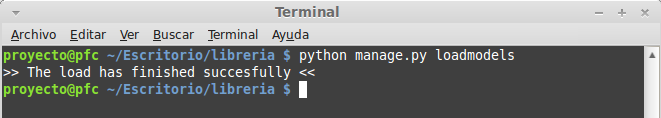
\includegraphics[width=1\textwidth]{manual_usuario/loadmodels.png}
    \end{center}
    \caption{Resultado de captación de modelos y fields}
    \label{fig:loadmodels}
\end{figure}

\subsection{Carga de namespaces}

El siguiente paso imprescindible para poder realizar el mapeo de sus modelos con
las ontologías, es tener alguna cargada en la aplicación. La carga de ontologías
o namespaces en la aplicación, se hace desde dentro de la aplicación, en el
apartado llamado Namespace.

Cuando acceda a este apartado, le aparecerá una lista con todos los namespaces
disponibles (Figura \ref{fig:lista_namespace}) para ser usados (inicialmente la
lista estará vacía). Desde este apartado, podrá tanto añadir nuevos namespaces
(Figura \ref{fig:nuevo_namespace}), como editarlos/actualizarlos (Figura
\ref{fig:editar_namespace}), o incluso eliminarlos\footnote{Tenga especial
cuidado a la hora de borrar los namespaces, ya que perderá también la
configuración que tenga entre sus modelos y el namespace. A la hora de borrar un
determinado namespace, se advertirá al usuario de que esté seguro de realizar
esta acción.}.

\newpage

\begin{figure}[H]
    \begin{center}
        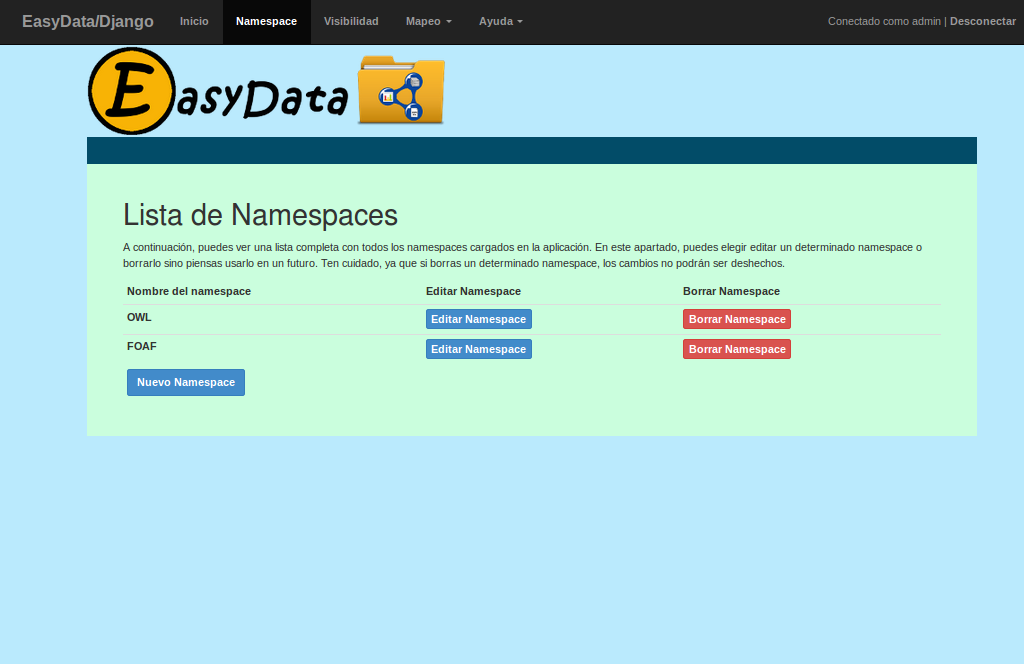
\includegraphics[width=0.9\textwidth]{manual_usuario/lista_namespace.png}
    \end{center}
    \caption{Listado de namespaces cargados en la aplicación}
    \label{fig:lista_namespace}
\end{figure}

\begin{figure}[H]
    \begin{center}
        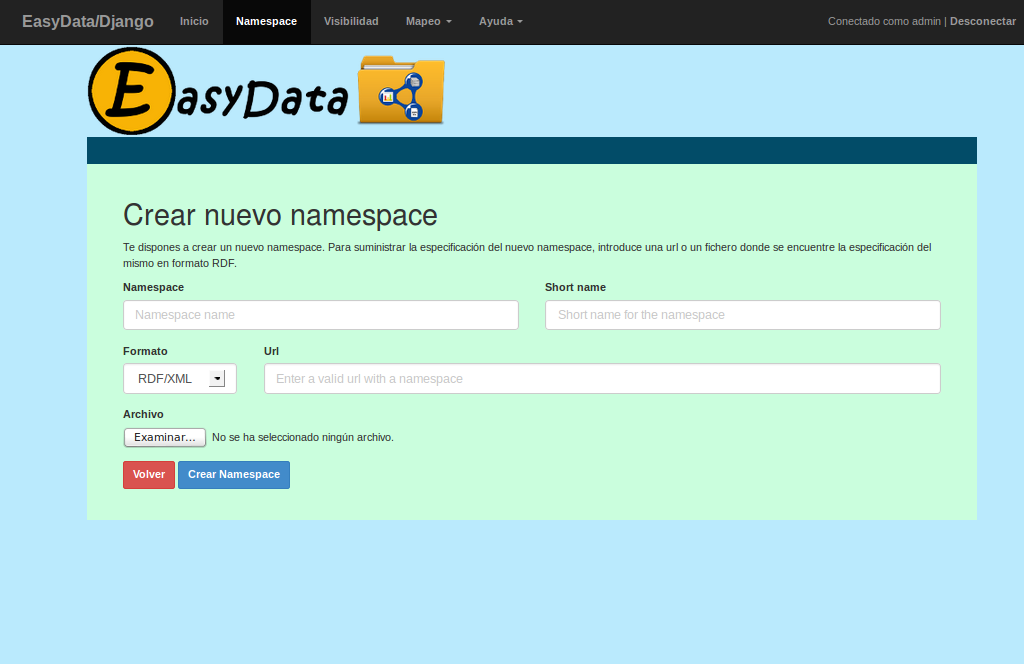
\includegraphics[width=0.9\textwidth]{manual_usuario/nuevo_namespace.png}
    \end{center}
    \caption{Formulario de creación de un nuevo namespace}
    \label{fig:nuevo_namespace}
\end{figure}

\begin{figure}[H]
    \begin{center}
        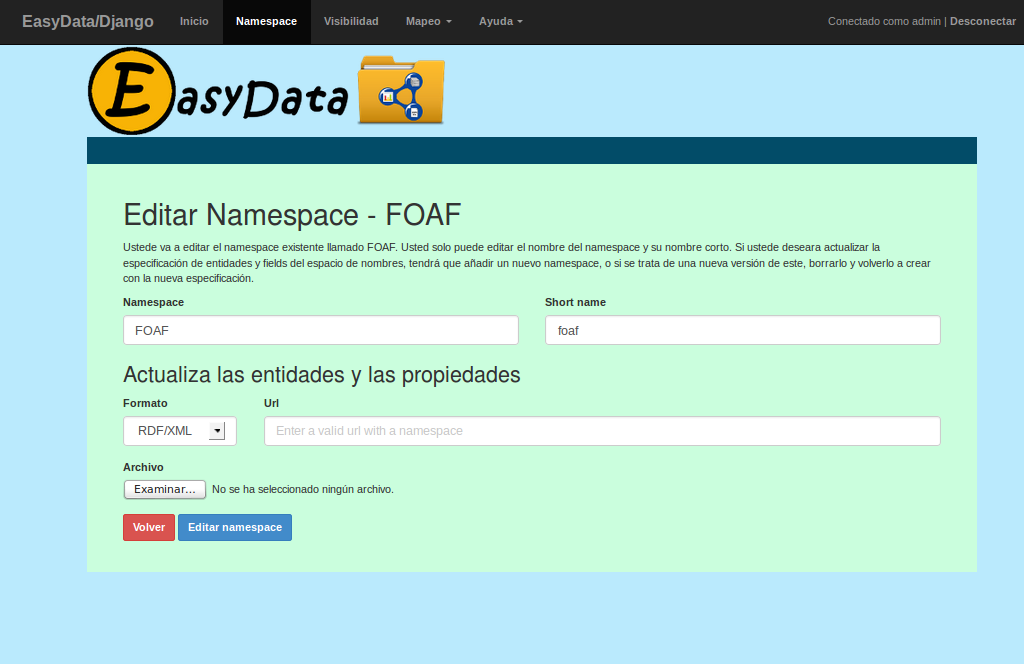
\includegraphics[width=0.9\textwidth]{manual_usuario/editar_namespace.png}
    \end{center}
    \caption{Pantalla de edición de un namespace existente}
    \label{fig:editar_namespace}
\end{figure}

Para cargar un nuevo namespace, pulse sobre el botón azul de
\textit{Nuevo Namespace}, y le aparecerá un formulario donde se le solicitará
la siguiente información:
\begin{itemize}
    \item \textbf{Namespace:} esto es un nombre identificativo que recibirá el
        namespace, el cual no influye en el mapeo. Este dato es único y no puede
        repetirse. Tiene como máximo 40 caracteres.
    \item \textbf{Short name:} este dato hace referencia a un nombre corto que
        represente el namespace, el cual se utilizará a la hora de generar tanto
        el RDF como RDFa, etc... Este dato es único y no puede repetirse con
        otros ya existentes. Tiene como máximo 15 caracteres.
    \item \textbf{Formato:} es el formato del fichero que se suministra con la
        especificación de la ontología. Actualmente están disponibles los
        formatos RDF/XML y RDF/Ntriples.
    \item \textbf{Url:} Es una url donde se encuentra el fichero con la
        especificación del namespace. Este dato no es obligatorio y solo debe
        suministrarse la url o el archivo.
    \item \textbf{Archivo:} Es un fichero donde se encuentra la especificación
        del namespace. Este dato no es obligatorio y solo debe suministrarse la
        url o el archivo.
\end{itemize}

Una vez introducidos los datos, pulse en \textit{Crear Namespace}, para cargar
el mismo en el sistema. Este proceso puede tardar un poco, en función del tamaño
del namespace, ya que se debe de leer toda la especificación y cargarla en la
base de datos.

Una vez se haya creado el namespace, se le redirigirá a la vista principal de
namespaces, y podrá observar que aparece en la lista el nuevo que acaba de
crear. Si por el contrario hubo algún error, se le informará y deberá de
corregir el formulario.

A la hora de editar/actualizar un namespace, le aparecerá un formulario similar
al de creación de un nuevo namespace, donde los campos nombre y short name,
aparecerán rellenos con los datos del namespace, de tal forma que pueda editar
los mismos. Por otro lado, también encontrará los apartados de formato, url y
archivo, donde para este caso, la utilidad de los mismos difiere un poco al del
caso anterior, ya que esta vez se cargará la especificación de las entidades y
propiedades del namespace, para añadir nuevas entidades o propiedades nuevas que
pudiesen haber sido incluidas posteriormente en la especificación, o para
actualizar las relaciones existentes entre entidades y propiedades del
namespace, con el resto de entidades y propiedades de otros namespaces
existentes en la aplicación, que no existiesen anteriormente.

Tanto a la hora de cargar un nuevo namespace como de actualizar uno existente,
esto se hará como bien se puede apreciar en el formulario, haciendo uso de
ficheros en formato rdf. Para que la aplicación pueda reconocer tanto las
entidades como las propiedades y las relaciones entre los mismos, estos deben de
estar especificados haciendo uso de las siguientes etiquetas defindas en los
namespaces \href{http://www.w3.org/TR/rdf-schema/}{RDFS} y
\href{http://www.w3.org/TR/owl-ref/}{OWL}:
\begin{itemize}
    \item Para la identificación de clases:
    \begin{itemize}
        \item \textbf{rdfs:Class}.
        \item \textbf{owl:Class}.
    \end{itemize}
    \item Para la identificación de propiedades:
    \begin{itemize}
        \item \textbf{rdf:Property}.
        \item \textbf{owl:ObjectProperty}.
        \item \textbf{owl:DatatypeProperty}.
        \item \textbf{owl:AnnotationProperty}.
    \end{itemize}
    \item Para la obtención de características de las clases y propiedades:
    \begin{itemize}
        \item \textbf{rdfs:comment}: para captar una descripción de la entidad o
            propiedad.
        \item \textbf{rdfs:label}: para captar la etiqueta de la entidad o
            propiedad.
        \item \textbf{rdfs:domain}: indica a qué entidades pertenece una
            determinada propiedad.
        \item \textbf{rdfs:range}: indica con qué entidades se relaciona una
            determinada propiedad.
        \item \textbf{rdfs:subClassOf}: indica de qué entidad es hija una
            determinada entidad.
    \end{itemize}
\end{itemize}

\subsection{Configuración de la privacidad}

Un punto muy importante a la hora de exportar nuestros datos, es decidir qué
datos queremos que se publiquen y qué otros no, ya que en muchos casos, nos será
interesante evitar que ciertos datos puedan ser accedidos por terceras personas,
porque se traten de datos sensibles, como contraseñas, números de cuentas
bancarias, etc... o sencillamente porque no deseemos que estos puedan verse.

La aplicación le permite la posibilidad de decidir qué datos se ocultaran a los
usuarios a la hora de publicar los mismos. Esto se hará en el apartado de
\textit{Visibilidad} (Figura \ref{fig:configura_visibilidad}). En este apartado,
le aparecerá un listado con cada una de las aplicaciones instaladas en su
proyecto Django, y pulsando en configurar visibilidad de una determinada
aplicación, se le mostrará una nueva pantalla (Figura
\ref{fig:configura_visibilidad_2}) con una pestaña por cada uno de los modelos
que contiene la aplicación.

\begin{figure}[H]
    \begin{center}
        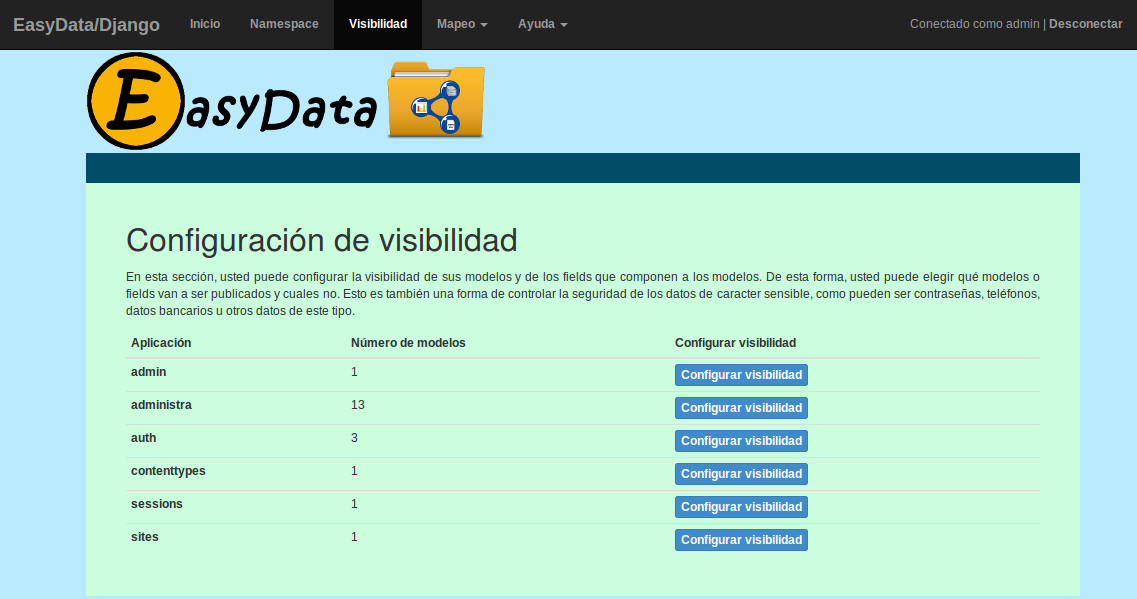
\includegraphics[width=0.95\textwidth]{manual_usuario/configura_visibilidad.png}
    \end{center}
    \caption{Pantalla de configuración de la privacidad - Aplicaciones}
    \label{fig:configura_visibilidad}
\end{figure}

En cada una de las pestañas de los modelos, podrá elegir si este modelo es
visible o privado completamente al exterior, o definirlo por fields en concreto,
indicando la visibilidad de los mismos.

Por defecto, para prevenir que inicialmente algún dato sea publicado por error,
todos los modelos están marcados como privados, de tal forma que será tarea del
usuario decidir cuáles de ellos se harán visibles.

\newpage

\begin{figure}[H]
    \begin{center}
        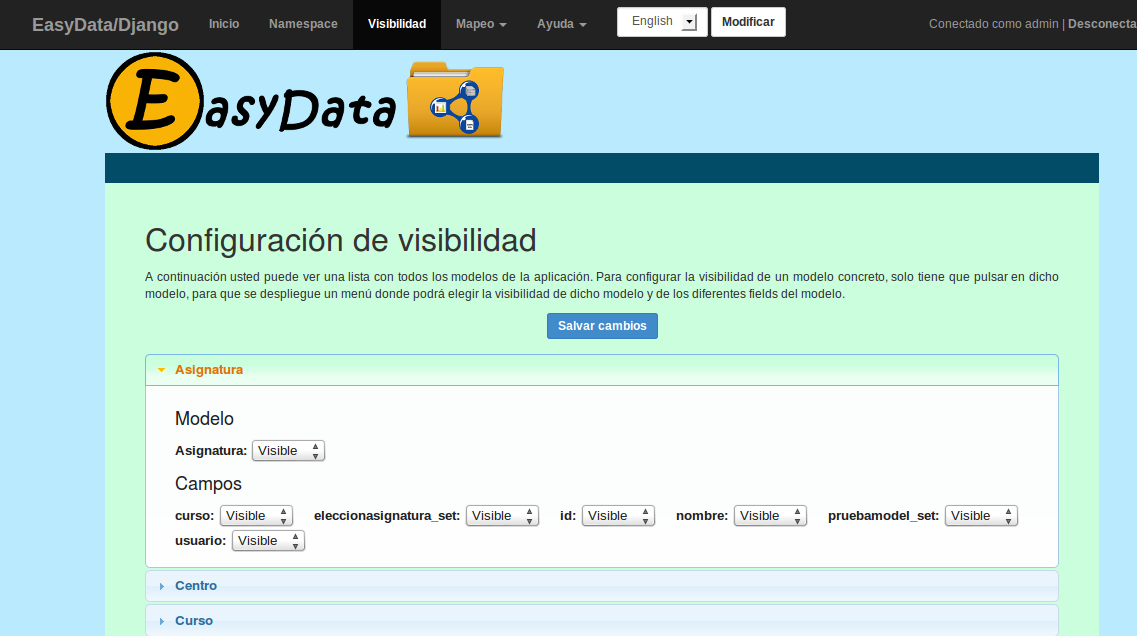
\includegraphics[width=0.95\textwidth]{manual_usuario/configura_visibilidad_2.png}
    \end{center}
    \caption{Pantalla de configuración de la privacidad - Modelos}
    \label{fig:configura_visibilidad_2}
\end{figure}

\subsection{Mapeo de modelos y fields}

El siguiente y último paso antes de la publicación de los datos, es indicarle a
la aplicación EasyData/Django, con qué entidades y propiedades de los distintos
namespaces van a estar relacionados nuestros modelos. Este paso se conoce como
el \textit{Mapeo de los datos}, y por consiguiente se llevará a cabo en el
apartado de la aplicación de \textit{Mapeo}.

Si accedemos a este apartado, nos aparecerá una lista desplegable (Figura
\ref{fig:mapea_modelos}). Cada uno de los elementos de la lista, representan a
cada una de las aplicaciones de nuestro proyecto. Si seleccionamos una de ellas,
para que se expanda dicho elemento, nos aparecerá cada uno de los modelos que
componen a dicha aplicación con dos elementos select. En esta parte realizaremos
el mapeo de los modelos, donde en el primero de los selects, seleccionaremos el
namespace que queremos utilizar de los que tenemos cargados en la aplicación, y
el siguiente select se cargará con las distintas entidades que componen al
namespace. De esta forma deberemos de mapear cada uno de los modelos que nos
interesen (no es necesario realizar el mapeo de todos, solo aquellos que nos
vaya a interesar publicar). Una vez realizado el mapeo de los modelos,
pulsaremos sobre el botón de \textit{Salvar cambios}.

\newpage

\begin{figure}[H]
    \begin{center}
        \includegraphics[width=1\textwidth]{manual_usuario/mapea_modelos.png}
    \end{center}
    \caption{Pantalla de mapeo de los modelos}
    \label{fig:mapea_modelos}
\end{figure}

Una vez hemos realizado el mapeo de los modelos y hemos salvado los cambios, se
activará el botón verde posicionado a la derecha de cada modelo que hemos
realizado su mapeo. Esto significa que podemos pasar ahora a realizar el mapeo
de los fields de dichos modelos, pulsando en dicho botón.

Cuando pulsemos sobre dicho botón, se nos llevará a un apartado parecido al
anterior, donde aparecerán por separado los atributos y relaciones del modelo
(Figura \ref{fig:mapea_fields}). Al igual que en el caso anterior, cada uno
dispondrá de dos selects, uno para elegir el namespace, y otro para elegir la
propiedad con la que deseamos mapear el field. Por defecto, aparece seleccionada
la entidad del namespace con que hemos mapeado el modelo, pero se puede
modificar para utilizar otras propiedades del mismo namespace u otro namespace
diferente.

Una vez se haya concluido con el mapeo de los field, igual que anteriormente con
los modelos, pulsaremos sobre el botón de \textit{Salvar cambios}, para que
estos queden registrados en la aplicación.

\newpage

\begin{figure}[H]
    \begin{center}
        \includegraphics[width=1\textwidth]{manual_usuario/mapea_fields.png}
    \end{center}
    \caption{Pantalla de mapeo de los fields de un determinado modelo}
    \label{fig:mapea_fields}
\end{figure}

\subsection{Publicación de los datos}

Una vez llegados a este punto, donde ya tenemos cargados los namespaces que
vamos a utilizar, tenemos configurada la privacidad de nuestros datos y el mapeo
de los mismos con los namespaces, solo queda publicar los datos de los mismos.

Para la publicación de los datos de los modelos de nuestro proyecto, existen
distintas posibilidades, según el formato y la vía a través de la cual
los queramos publicar:
\begin{itemize}
    \item A través de url generadas para instancias en concreto de los modelos,
    para todas las instancias de un modelos, o para todos los modelos mapeados
    con una determinada entidad de un namespace.
    \item Mediante código HTML, usando los formatos para el marcado de
    etiquetas HTML, como son RDFa y Microdata.
    \item A través de la plataforma D2Rq haciendo uso del endpoint SPARQL que
    ofrece.
\end{itemize}

\subsubsection{Mediante URLs}

Como hemos comentado anteriormente, una de las posibles formas que hay para
publicar los datos de su aplicación es a través del uso de URLs. Estas URLs
servirán sus datos en formatos como puede ser RDF/XML, RDF/Ntriples o
RDF/Trutle.

Para los ejemplos, supondremos que nuestro proyecto se encuentra instalado en la
URL 127.0.0.1:8000.

La aplicación EasyData/Django creará automáticamente tres tipos diferentes de
URLs:
\begin{itemize}
    \item URLs específicas para instancias concretas de cada uno de los modelos.
        Estas URLs están compuestas de la aplicación, el tipo (la entidad),
        modelo y clave primaria de la instancia, de la siguiente forma:
    \begin{center}
        \textit{http://127.0.0.1:8000/easydata/publish/instance/\textbf{aplicación}/\textbf{tipo}-\textbf{modelo}/\textbf{pk}.(xml|nt|ttl)}
    \end{center}
        Donde las palabras marcadas en negrita, se sustituirán por los datos
        comentados anteriormente, y la clave primaria irá seguida del formato en
        el que deseamos recibir los datos.
    \item También se crearán URLs concretas para cada modelo de nuestro
        proyecto, de tal forma que nos devolverá un fichero RDF con cada una de
        las instancias de dicho modelo. Dicha URL será de la siguiente forma:
    \begin{center}
        \textit{http://127.0.0.1:8000/easydata/publish/model/\textbf{aplicación}/\textbf{tipo}-\textbf{modelo}.(xml|nt|ttl)}
    \end{center}
        Donde las palabras marcadas en negrita, se sustituirán por los nombres
        de la aplicación y del modelo, seguido el modelo del formato en el que
        deseamos recibir los datos.
    \item Por último, también se crearán URLs concretas para cada una de las
        entidades de los namespaces, de tal forma que nos devolverá un fichero
        RDF con cada una de las instancias de los modelos mapeados con dicha
        entidad. Dicha URL tendrá el siguiente formato:
    \begin{center}
        \textit{http://127.0.0.1:8000/easydata/publish/type/\textbf{namesapace}/\textbf{entidad}.(xml|nt|ttl)}
    \end{center}
        Donde la palabra namespace, se sustituirá por el nombre del namespace y
        la palabra entidad por el nombre de la entidad de la que queremos
        obtener los datos en RDF, seguido del formato RDF en el que queremos que
        nos muestre los datos.
\end{itemize}

Para obtener información mucho mas concreta sobre todo lo comentado
anteriormente, puede consultar los apartados \textit{Modelos configurados} y
\textit{Entidades relacionadas} de la ayuda de la aplicación, donde se le
muestra todo lo comentado anteriormente, con ejemplos sobre datos reales de su
proyecto.

\subsubsection{Mediante RDFa y Microdata}

Para la inclusión de los datos en formato HTML en nuestras plantillas de Django,
se hará uso de los template tags de Django, que no son mas que funciones, que
pueden ejecutarse desde las plantillas.

Estos template tags, son funciones que reciben una determinada instancia de un
modelo, y generarán el html con las etiquetas RDFa o Microdata (siempre que el
modelo de la instancia haya sido mapeado previamente), de tal forma que cuando
una máquina acceda a nuestra aplicación, sea capaz de interpretar dichas marcas
como si de un fichero RDF se tratara y pueda interpretar la información de la
misma.

A continuación se indican los template tags disponibles, tanto para la
generación de código RDFa como Microdata.

\begin{center}
    \textbf{Microdata}
\end{center}

Para poder hacer uso de los template tags para la generación de código
Microdata, se deberá de cargar en la plantilla Django el módulo donde se
encuentran los template tags, incluyendo el siguiente código:

\begin{center}
    \textit{\{\% load easydata\_microdata \%\}}
\end{center}

Una vez tenemos cargados los template tags para microdata, únicamente tendremos
que hacer uso en las plantillas de ellos. Los template tags para microdata
disponibles son los siguientes:

En el caso de que queramos generar el código microdata de una determinada
instancia de un modelo y que muestre todos los fields visibles y mapeados de
este:
\begin{center}
    \textit{\{\% microdata\_ul instance \%\}}\\
    \textit{\{\% microdata\_div\_meta instance \%\}}\\
    \textit{\{\% microdata\_div\_span instance \%\}}\\
\end{center}

En el caso de que queramos generar el código microdata de una instancia,
indicándole el field en concreto que deseamos que muestre:
\begin{center}
    \textit{\{\% microdata\_li\_field instance ``field\_name'' \%\}}\\
    \textit{\{\% microdata\_meta\_field instance ``field\_name'' \%\}}\\
    \textit{\{\% microdata\_span\_field instance ``field\_name'' \%\}}\\
\end{center}

Cuando se hace uso de los templatetags que genera información de un determinado
field de la instancia, solo se genera la etiqueta HTML con el tipo del dato y el
dato en cuestión, por lo que no se incluye información del tipo de la instancia
a la que pertenece el dato, y que deberá incluir el usuario. Para ello, existe
un template tag de bloque que indicándole la instancia y el tipo de etiqueta que
queremos usar, nos genera dicha etiqueta de apertura y cierre HTML con la
información Microdata del tipo de la instancia. La estructura de este template
tag es la siguiente:
\begin{center}
    \textit{\{\% microdata\_open\_tag instance ``tag'' \%\}}\\
    Resto de etiquetas de la instancia\\
    \textit{\{\% microdata\_end\_tag \%\}}\\
\end{center}

A su vez, puede que una determinada instancia de un modelo de datos, contenga
relaciones con otra instancia de otro modelo, que por defecto al generar el
código HTML con Microdata, lo que se hará será generar una etiqueta con la
referencia a la URI que representa a la instancia con la que se relaciona. Puede
que sea de interés para el usuario, que en vez de dicha referencia, se generen
determinados datos de la instancia indicando la relación de esta (anidar
instancias). Para ello, existe también un template tag de bloque similar al
anterior, donde se indican las instancias relacionadas, el nombre del field y la
etiqueta mediante la cual relacionarlos. La estructura de este template tag es
la siguiente:
\begin{center}
    \textit{\{\% microdata\_open\_tag\_interno instancia\_padre instancia ``field'' ``tag'' \%\}}\\
    Resto de etiquetas de la instancia\\
    \textit{\{\% microdata\_end\_tag\_interno \%\}}\\
\end{center}

\begin{center}
    \textbf{RDFa}
\end{center}

Para poder hacer uso de los template tags para la generación de código RDFa, se
deberá de cargar en la plantilla Django el módulo donde se encuentran los
template tags, incluyendo el siguiente código:

\begin{center}
    \textit{\{\% load easydata\_rdfa \%\}}
\end{center}

Una vez tenemos cargados los template tags para RDFa, únicamente tendremos que
hacer uso en las plantillas de ellos. Los template tags para RDFa disponibles
son los siguientes:

En el caso de que queramos generar el código RDFa con una instancia y que
muestre todos los fields visibles y mapeados de este:
\begin{center}
    \textit{\{\% rdfa\_ul instance \%\}}\\
    \textit{\{\% rdfa\_div instance \%\}}\\
    \textit{\{\% rdfa\_div\_span instance \%\}}\\
\end{center}

En el caso de que queramos generar el código RDFa con instancias e
indicándole el field en concreto que deseamos que muestre:
\begin{center}
    \textit{\{\% rdfa\_li\_field instance ``field\_name'' \%\}}\\
    \textit{\{\% rdfa\_div\_field instance ``field\_name'' \%\}}\\
    \textit{\{\% rdfa\_span\_field instance ``field\_name'' \%\}}\\
\end{center}

Cuando se hace uso de los templatetags que genera información de un determinado
field de la instancia, solo se genera la etiqueta HTML con el tipo del dato y el
dato en cuestión, por lo que no se incluye información del tipo de la instancia
a la que pertenece el dato, y que deberá incluir el usuario. Para ello, existe
un template tag de bloque que indicándole la instancia y el tipo de etiqueta que
queremos usar, nos genera dicha etiqueta de apertura y cierre HTML con la
información RDFa del tipo de la instancia. La estructura de este template tag es
la siguiente:
\begin{center}
    \textit{\{\% rdfa\_open\_tag instance ``tag'' \%\}}\\
    Resto de etiquetas de la instancia\\
    \textit{\{\% rdfa\_end\_tag \%\}}\\
\end{center}

A su vez, puede que una determinada instancia de un modelo de datos, contenga
relaciones con otra instancia de otro modelo, que por defecto al generar el
código HTML con RDFa, lo que se hará será generar una etiqueta con la
referencia a la URI que representa a la instancia con la que se relaciona. Puede
que sea de interés para el usuario, que en vez de dicha referencia, se generen
determinados datos de la instancia indicando la relación de esta (anidar
instancias). Para ello, existe también un template tag de bloque similar al
anterior, donde se indican las instancias relacionadas, el nombre del field y la
etiqueta mediante la cual relacionarlos. La estructura de este template tag es
la siguiente:
\begin{center}
    \textit{\{\% rdfa\_open\_tag\_interno instancia\_padre instancia ``field'' ``tag'' \%\}}\\
    Resto de etiquetas de la instancia\\
    \textit{\{\% rdfa\_end\_tag\_interno \%\}}\\
\end{center}

Para obtener información más detallada sobre el uso de los template tags, puede
dirigirse al apartado de \textit{Uso en plantillas} de la ayuda de la
aplicación, donde podrá observar todos los template tags disponibles, así como
ejemplos de uso de cada uno y resultado generado, sobre datos reales de sus
modelos.

\subsubsection{Enlace en HTML}

Además de los template tags comentados anteriormente, dispone de un template tag
más, el cual a partir de una instancia de un modelo, genera el código HTML de un
enlace ``<a>'' con la URI donde se encuentra la información RDF de la instancia
que se le indicó.

Para hacer uso de este template tag, debe de importarlo de la siguiente forma:

\begin{center}
    \textit{\{\% load easydata\_links \%\}}
\end{center}

Y por último, el template tag se usará dentro de la plantilla Django de la
siguiente forma:

\begin{center}
    \textit{\{\% easydata\_include\_link instance \%\}}
\end{center}


\subsection{Generación de fichero D2Rq}

La plataforma D2RQ de código abierto, es un sistema para el acceso a los datos
de bases de datos relacionales, como si se tratasen de grafos RDF virtuales de
solo lectura. De esta forma, ofrece a los usuario acceso mediante RDF al
contenido relacional de las bases de datos, sin la necesidad de tener que
replicar estos sobre un almacenamiento en formato RDF. Resumiendo, haciendo uso
de D2RQ podrás:
\begin{itemize}
    \item Hacer consultas sobre una base de datos que no sea de tipo RDF
        haciendo uso de SPARQL.
    \item Acceder al contenido de la base de datos, como Linked Data sobre la
        web.
    \item Crear volcados personalizados de la base de datos en formato RDF.
    \item Acceder a información de una base de datos que no sea de tipo RDF,
        haciendo uso de la API Apache Jena.
\end{itemize}

Para realizar las tareas anteriormente citadas, el software D2Rq necesita de un
fichero de configuración, donde se plasme el mapeo entre las tablas y columnas
de la base de datos y las etiquetas de los distintos namespaces, de forma que
este software pueda procesar las consultas SPARQL y crear el contenido RDF. Este
fichero, puede ser generado en la aplicación EasyData/Django, haciendo uso del
mapeo realizado en la propia aplicación.

Para realizar dicho mapeo, al igual que cuando realizó la resolución de los
modelos y fields del proyecto, deberá ejecutar desde la terminal el siguiente
comando del manage.py de Django.

\begin{lstlisting}[frame=L, language=bash, basicstyle=\footnotesize]
$> python manage.py easydata_d2rq
\end{lstlisting}

Este comando le mostrará por pantalla la configuración en formato
\textit{Turtle} (ttl) realizada por usted en la aplicación lista para ser usada
en la aplicación D2Rq. Si desea guardar la configuración en un fichero, solo
tiene que redirigir la salida hacia un fichero de la siguiente forma:

\begin{lstlisting}[frame=L, language=bash, basicstyle=\footnotesize]
$> python manage.py easydata_d2rq > configuracion.ttl
\end{lstlisting}

Una vez generado el fichero, deberá editarlo mediante cualquier editor
compatible con este formato de fichero, para introducir las opciones de conexión
a la base de datos (nombre de usuario, contraseña, host, controlador, etc...).
Además, este se trata de un documento base con la estructura que hay definida de
la base de datos dentro de la aplicación, el cual usted podrá editar para añadir
nuevos tipos de relaciones, propiedades, etc...

Tenga en cuenta que el software D2Rq es bastante complejo y ofrece al usuario
una gran cantidad de posibilidades a la hora de trabajar con los datos y
realizar el mapeo de los mismo. Además, este software trabaja directamente sobre
la estructura de la base de datos y esta en los proyectos Django se encuentra
estructurada en función de la forma de trabajar del ORM del framework, de tal
forma que no siempre se corresponderán los modelos con las tablas existentes en
la base de datos, principalmente cuando existan herencias y relaciones
complejas. Por estas dos razones, el resultado final del fichero puede no ser
definitivo, sino que servirá como base para que el usuario no tenga que trabajar
desde un fichero completamente en blanco y pueda aprovechar gran parte del
trabajo realizado sobre la aplicación, pero este requerirá finalmente de la
intervención del usuario.

Finalmente, una vez tenga el fichero de configuración para D2Rq podrá realizar
multitud de acciones, como desplegar un servidor donde los usuarios puedan
consultar los datos publicados. Este servidor podrá ser desplegado directamente
desde la línea de comandos (\url{http://d2rq.org/d2r-server#command-line}), o
bien como una aplicación web J2EE dentro de un servidor Apache Tomcat o Jetty
(\url{http://d2rq.org/d2r-server#servlet-container}).

Para más información acerca de cómo realizar consultas, modificar los ficheros
de configuración D2Rq, ejecución del servidor web, y el resto de utilidades y
herramientas que le proporciona la plataforma D2Rq, consulte la página oficial
\cite{d2rq} donde se le explica todo esto mucho más detallado.

\subsection{Generación de gráfico}

A la vez que vaya realizando el mapeo de sus modelos y fields con las
correspondientes entidades y propiedades de los namespaces, podrá obtener un
grafo donde podrá visualizar dicha configuración. En ella se apreciarán cada uno
de los modelos con sus atributos, así como las relaciones existentes entre
modelos, y junto a cada uno de ellos, las entidades o propiedades de los
namespaces con las que están mapeados.

Para generar dicho grafo, deberá de hacer click sobre el apartado de
\textit{Mapeo}, y en el menú desplegable que le aparece, pulsar sobre la opción
de \textit{Generar grafo}. Automáticamente, la aplicación le devolverá un
fichero .png con el grafo indicado.

En caso de que el sistema no disponga de la aplicación GraphViz para la
generación de la imagen png, se le devolverá un fichero en formato .dot, a
partir del cual, podrá generar la imagen haciendo uso de la aplicación graphviz.
Para generar la imagen desde la interfaz gráfica de la aplicación graphviz, o
desde una terminal de escritorio, donde tendrá que ejecutar el siguiente
comando:

\begin{lstlisting}[frame=L, language=bash, basicstyle=\footnotesize]
$> dot grafo.dot -Tpng -o nombre_grafo.png
\end{lstlisting}

% TODO: cuando sepa exactamente si se incluirá esta parte

% Descripción del área de trabajo del sistema y las instrucciones concretas para hacer uso de las funcionalidades del sistema.


\chapter{Conclusiones}
% ------------------------------------------------------------------------------
% Este fichero es parte de la plantilla LaTeX para la realización de Proyectos
% Final de Grado, protegido bajo los términos de la licencia GFDL.
% Para más información, la licencia completa viene incluida en el
% fichero fdl-1.3.tex

% Copyright (C) 2012 SPI-FM. Universidad de Cádiz
% ------------------------------------------------------------------------------

En este último capítulo se detallan las lecciones aprendidas tras el desarrollo
del presente proyecto y se identifican las posibles oportunidades de mejora
sobre el software desarrollado.

\section{Objetivos}

A continuación, se recoge una valoración de los objetivos planteados
inicialmente en la sección \ref{sec:objetivos} que debería de recoger el
proyecto y los objetivos que se han alcanzado una vez finalizado el proyecto:
\begin{itemize}
    \item Se han implementado una serie de modelos de Django los cuales se
        encargan de almacenar tanto la información de los distintos namespaces
        cargados en la aplicación junto con las entidades y propiedades que
        componen a estos, como la información acerca de los diferentes modelos
        que componen a las aplicaciones del proyecto Django junto con los fields
        de los mismos. De esta forma se satisface el primer subobjetivo
        planteado en el objetivo \textbf{OBJ-001}.
    \item Se ha desarrollado un script y agregado este al manage.py de Django,
    	que se encarga de realizar la resolución de los distintos modelos que
        componen al proyecto, así como los fields (atributos y relaciones) de
        cada uno de estos. Con esto se satisface el segundo subobjetivo
        planteado en el objetivo \textbf{OBJ-001}.
    \item Además, el procedimiento anterior, también permite actualizar la
        especificación de los modelos y sus fields una vez que estos ya han sido
        cargados, cuando se realicen cambios en los mismos. Como por ejemplo,
        que se agregue o elimine algún modelo o field. De esta forma, se amplía
        la funcionalidad descrita por el objetivo \textbf{OBJ-001}.
    \item Se ha desarrollado un apartado donde el usuario puede añadir nuevos
        namespaces u ontologías a la aplicación. Además, dicho apartado también
        permite eliminar los namespaces incluidos, y actualizar la
        especificación de los mismos. De esta forma, se satisface el primer
        subobjetivo del objetivo \textbf{OBJ-002}.
    \item Se ha desarrollado otro apartado donde se permite al usuario realizar
        la correspondencia entre los distintos modelos y fields de nuestro
        proyecto, con los diferentes vocabularios que se han cargado en la
        aplicación. De esta forma se satisface los subobjetivos segundo y
        tercero del objetivo \textbf{OBJ-002}.
    \item También se ha desarrollado un apartado donde el usuario puede realizar
    	la configuración de la visibilidad de cada uno de los modelos y fields
    	que existen en el proyecto Django, de forma que no se permita publicar
        información no deseada. Con esto se satisface el cuarto subobjetivo del
        objetivo \textbf{OBJ-002}.
    \item Se han creado además, dos nuevos apartados donde se puede generar un
        fichero de configuración para utilizar con la plataforma D2Rq y también
        permite descargar un gráfico con la configuración que se ha realizado
        sobre los modelos de nuestro proyecto. Con esto se mejora la
        especificación del objetivo \textbf{OBJ-002}.
    \item Se han desarrollado herramientas que permiten la publicación de los
        datos de los modelos del proyecto Django, en multitud de formatos, como
        pueden ser RDF/XML, RDF/Ntriples, RDF/Turtle, RDFa o Microdata, además
        de herramientas para la generación de enlaces a los datos de las
        instancias de los modelos e inserción de información en plantillas
        Django. De esta forma, se satisface el objetivo \textbf{OBJ-003}.
\end{itemize}

% Este apartado debe resumir los objetivos generales y específicos alcanzados, relacionándolos con todo lo descrito en el capítulo de introducción.\\

\section{Lecciones aprendidas}

A continuación se detallan las buenas prácticas adquiridas, tanto tecnológicas
como procedimentales. Por ello, podemos decir que a nivel tecnológico, se ha
adquirido un mayor dominio y conocimiento del framework de desarrollo Django, de
su funcionamiento interno y de las diferentes herramientas que este presta al
usuario. Además, también se han obtenido nuevos conocimientos en tecnologías como
SPARQL, D2Rq, RDF y web semántica. En general, al haber sido realizado todo bajo
el lenguaje de programación Python, se ha obtenido un mayor dominio de este
lenguaje, se han conocido nuevas librerías disponibles en el
\textit{Python Package Index} y características que ofrece el lenguaje, como
puede ser la introspección. Además, en el ámbito del desarrollo web, también he
tenido que hacer uso de otras tecnologías, ya conocidas anteriormente, pero que
me ha ayudado a ampliar mis conocimientos sobre ellas, así como el uso de otros
frameworks, para el contenido tanto CSS como JavaScript.

Además de todos los conocimientos tecnológicos adquiridos, también se han
obtenido buenas prácticas a la hora de programar y organizar el trabajo. Esto se
ha conseguido siguiendo la guía de estilos PEP8 y la herramienta PyLint a la
hora de realizar la implementación del proyecto, lo cual es importante, ya que
asegura que el código será mantenible y comprensible por cualquier usuario que
esté habituado a trabajar siguiendo estas normas de estilo.

También se han puesto en práctica los conocimientos adquiridos tanto en mis
estudios de Ingeniería Técnica en Informática de Sistemas como en Ingeniería
Informática, ya que estos me han sido necesarios para la elaboración del
proyecto, tanto en el apartado de análisis y diseño de requisitos, prototipado,
análisis de riesgos, como en el apartado de implementación, haciendo uso de las
buenas prácticas adquiridas, como por ejemplo el uso de patrones de diseño.

Por último, a nivel organizativo, se ha seguido una guía metodológica haciendo
uso de un lenguaje de modelado de procesos, donde se describen y priorizan cada
una de las etapas del proyecto. Se ha realizado un análisis y diseño del
proyecto, así como una planificación de riesgos y temporal del proyecto. En
dicho estudio temporal del proyecto, el cual se puede ver el resultado en el
diagrama de Gantt del apartado de análisis (Figura \ref{fig:GanttInicial}), se
le asignaba al proyecto una duración estimada de 12 meses, comenzado el
desarrollo del mismo en Octubre de 2012, teniendo en cuenta que la dedicación al
mismo no sería total y el resto de riesgos que pudiesen surgir. De esta forma,
se ha aprendido la importancia de la gestión de los proyectos, de la estimación
temporal y del esfuerzo de los mismos y de la realización de un análisis y
diseño del mismo, de tal forma que se verá reflejado en una mejor administración
de los recursos y cumplimiento de plazos.

% Este apartado debe recoger una comparación cuantitativa del tiempo y el esfuerzo realmente invertido frente al estimado y planificado. Estos datos pueden recogerse del sistema de gestión de tareas empleado para el seguimiento del proyecto. Es mejor resumir cuantitativamente el tiempo y esfuerzo dedicados al proyecto a lo largo de su desarrollo y medido de esta forma que escribir un sencillo ``he trabajado mucho en este proyecto''.


\section{Trabajo futuro}

Una vez concluido el proyecto y obtenida la primera versión del software
EasyData/Django, a raíz de la experiencia obtenida a lo largo del desarrollo del
mismo, se han podido observar una serie de mejoras o ampliaciones, en cuya
dirección podría ir orientado el trabajo futuro para la aplicación. Estas
ampliaciones aportarían a la aplicación un mayor valor para el usuario,
aumentando las funcionalidades de la misma.

A continuación se muestra una lista de posibles mejoras en las que podría ir
encaminado el trabajo futuro:
\begin{itemize}
    \item Posibilidad de poder realizar más de una configuración simultánea de
        los modelos de la aplicación, con los namespaces cargados en la misma.
        De este modo se ofrecería al usuario mayor versatilidad a la hora de
        publicar sus datos en la web.
    \item Incluir un endpoint de SPARQL propio, que funcione desde la misma
    	aplicación de Django, que sustituya al fichero D2Rq que se genera
    	actualmente, quedando todo integrado en la misma aplicación. De igual
    	forma, si se desarrollase este módulo, se podría considerar la
    	posibilidad de que no sólo pudiesen realizarse consultas, sino también
        inserciones y modificaciones de los datos.
    \item Ampliar los formatos de exportación de datos respecto de los que
        pueden usarse actualmente (RDF, RDFa y Microdata), usando otros formatos
        existentes como por ejemplo JSON-LD además de ampliar los existentes.
    \item Ampliar la disponibilidad de la aplicación EasyData (actualmente
        existente para Ruby on Rails y Django) a otros frameworks de desarrollo
        web que sean ampliamente utilizados actualmente.
\end{itemize}

Si bien, todas las posibles mejoras no requieren un mismo esfuerzo, ya que
mejoras como las de la creación de un módulo propio para la realización de
consultas haciendo uso del lenguaje SPARQL es bastante ambicioso y complejo, el
cual requiere de un gran trabajo, tanto de investigación como de desarrollo, ya
que habría que estudiar primeramente como funciona el ORM de Django, para
posteriormente adaptar las consultas SPARQL a este. Además, si se tratase la
posibilidad de realizar inserciones y modificaciones en la base de datos, habría
que gestionar de alguna forma los permisos de los usuarios para realizar las
mismas.

Por otro lado, mejoras como la exportación de la aplicación a otros frameworks
de desarrollo web, habría que estudiar entre las posibilidades de realizar una
nueva aplicación para el framework en concreto, o la posibilidad de adaptar la
existente a cualquier framework. O al menos agrupar estos por lenguajes de
programación, como por ejemplo, en el caso de Python, existen varios frameworks
de desarrollo web además de Django, como puede ser Web2Py, Zope, etc... por lo
que también se podría estudiar la posibilidad de desarrollar un paquete de Python
que sirviese para la mayoría de los frameworks web de Python.

% En esta sección, se presentan las diversas áreas u oportunidades de mejora detectadas durante el desarrollo del proyecto y que podrán ser abarcadas en futuras versiones del software.\\

% Los elementos aquí descritos deben estar en relación con lo relatado en el apartado de objetivos y alcance del proyecto descritos en la introducción.\\



% Apéndice
\appendix
\chapter{Tablas del apartado de análisis}
En este apartado se van a plasmar cada una de las tablas que se han desarrollado
para el apartado de análisis de requisitos del proyecto.

\section{Tablas de requisitos funcionales}

A continuación se muestran cada una de las tablas donde se indican cada uno de
los requisitos de funcionales que debe de implementar el proyecto.

\subsection{Carga de modelos}

%%%TABLA - Caso de uso 001
\begin{center}
\begin{longtable}{||p{3.4cm}|p{12cm}||}
%primera parte de la tabla
 \hline \hline \bf UC-001 &  \bf Carga de modelos \\
\hline
\endfirsthead
%primera parte de la tabla por pagina
\hline \multicolumn{2}{|r|}{{Continuación de la tabla}} \\ \hline
 \hline \bf UC-001 &  \bf Carga de modelos \\
\hline
\endhead
% ultima parte de la tabla por pagina
\hline \multicolumn{2}{|l|}{{Continúa en la siguiente página}} \\ \hline
\endfoot
% ultima parte de la tabla
\endlastfoot
% DATOS
 \hline \bf Autor & José Manuel Llerena Carmona \\
 \hline \bf Descripción & Carga de modelos y fields del proyecto Django
             donde se va a usar la aplicación.\\
 \hline \bf Actores & Administrador del sistema\\
 \hline \bf Precondición & Se ha configurado la aplicación en el proyecto
             Django, la aplicación posee una base de datos y se han sincronizado
             las modelos de la aplicación con la base de datos de la aplicación
             para que se creen las tablas necesarias.\\
 \hline \bf Postcondición & Se han cargado en las tablas de la base de datos
             correspondiente a la aplicación los modelos y fields de estos.\\
 \hline \bf Secuencia normal & 
             \begin{enumerate}
                \item El administrador accede a través de la línea de comandos
                       de la terminal al path donde se encuentra el proyecto Django.
                \item El administrador ejecuta el script que se encarga de
                       cargar los modelos y fields existentes en la aplicación
                       Django.
                \item El sistema indica al administrador que los datos se han
                       cargado correctamente.
             \end{enumerate}\\
 \hline \bf Excepciones &
             \begin{description}
                \item[3.1] Existen modelos ya cargados en la base de datos, por
                            lo que el sistema actualiza dichas tablas y añade
                            las que no existan.
                \item[3.2] La aplicación no tiene configurada una base de datos
                            o sus modelos no están configurados correctamente.
                            La aplicación aborta el procedimiento de carga de
                            modelos y muestra mensaje de error.
             \end{description}\\
\hline
\hline
\caption{\label{tab:caso001} Caso de Uso - 001 - Carga de modelos} 
\end{longtable}
\end{center}


\subsection{Carga de espacios de nombres}

%%%TABLA - Caso de uso 002
\begin{center}
\begin{longtable}{||p{3.4cm}|p{12cm}||}
%primera parte de la tabla
 \hline \hline \bf UC-002 &  \bf Carga de espacios de nombres \\
\hline
\endfirsthead
%primera parte de la tabla por pagina
\hline \multicolumn{2}{|r|}{{Continuación de la tabla}} \\ \hline
 \hline \bf UC-002 &  \bf Carga de espacio de nombres \\
\hline
\endhead
% ultima parte de la tabla por pagina
\hline \multicolumn{2}{|l|}{{Continúa en la siguiente página}} \\ \hline
\endfoot
% ultima parte de la tabla
\endlastfoot
% DATOS
 \hline \bf Autor & José Manuel Llerena Carmona \\
 \hline \bf Descripción & Se debe de realizar una serie de procedimientos los
             cuales permitan a la aplicación cargar la estructura de los
             diferentes namespaces existentes, además de permitir actualizar y
             eliminar estos.\\
 \hline \bf Actores & Administrador del sistema\\
 \hline \bf Precondición & Se ha configurado la aplicación en el proyecto
             Django, la aplicación posee una base de datos y se han sincronizado
             las modelos de la aplicación con la base de datos de la aplicación
             para que se creen las tablas necesarias.\\
 \hline \bf Postcondición & Se han cargado en las tablas de la base de datos
             correspondientes a la aplicación las distintas entidades que
             componen al namespaces y los atributos de cada una de estas
             entidades.\\
 \hline \bf Secuencia normal & 
             \begin{enumerate}
                \item El administrador sistema accede al listado de namespaces
                       disponibles.
                \item El sistema muestra el listado de namespaces existentes en
                       la aplicación.
                \item El administrador del sistema selecciona crear un nuevo
                       namespace.
                \item El sistema muestra al administrador un formulario para
                       crear un nuevo namespace.
                \item El administrador del sistema indica los datos del nuevo
                       namespace, así como el fichero o la URL donde se
                       encuentra la especificación de dicho namespace.
                \item El sistema carga la especificación del namespace en la
                       base de datos, y muestra por pantalla el resultado de la
                       carga.
             \end{enumerate}\\
 \hline \bf Excepciones &
             \begin{description}
                \item[*.1] El administrador del sistema puede cancelar en
                          cualquier momento el procedimiento de
                          carga/actualización de los namespaces.
                \item[*.2] El usuario no tiene permisos de superusuario.
                \item[3.1] El usuario indica editar un namespace, para
                          actualizar su nombre o actualizar la especificación
                          mediante un fichero o URL.
                \item[6.1] La URL o fichero especificado por el usuario no es
                          correcta, y no se encuentra en ella una estructura de
                          namespaces, o dichos datos no son correctos.
                \item[6.2] Los nombres suministrados para el namespace ya están
                          siendo usados. El sistema vuelve a solicitar un nombre
                          correcto.
             \end{description}\\
\hline
\hline
\caption{\label{tab:caso002} Caso de Uso - 002 - Carga de espacios de nombres}
\end{longtable}
\end{center}


\subsection{Mapeo de modelos}

%%%TABLA - Caso de uso 003
\begin{center}
\begin{longtable}{||p{3.4cm}|p{12cm}||}
%primera parte de la tabla
 \hline \hline \bf UC-003 &  \bf Mapeo de modelos \\
\hline
\endfirsthead
%primera parte de la tabla por pagina
\hline \multicolumn{2}{|r|}{{Continuación de la tabla}} \\ \hline
 \hline \bf UC-003 &  \bf Mapeo de modelos \\
\hline
\endhead
% ultima parte de la tabla por pagina
\hline \multicolumn{2}{|l|}{{Continúa en la siguiente página}} \\ \hline
\endfoot
% ultima parte de la tabla
\endlastfoot
% DATOS
 \hline \bf Autor & José Manuel Llerena Carmona \\
 \hline \bf Descripción & Este caso de uso describe el procedimiento mediante
             el cual el administrador del sistema, describe en la aplicación la
             relación de cada uno de los modelos del proyecto Django, con las
             entidades de los distintos namespaces que existen en la
             aplicación.\\
 \hline \bf Actores & Administrador del sistema\\
 \hline \bf Precondición & Se ha cargado en la aplicación los modelos y
             atributos existentes en el proyecto, y además existe algún namespace
             cargado en la aplicación, de forma que se dispongan entidades y
             propiedades con el que mapear los modelos.\\
 \hline \bf Postcondición & Uno o varios de los modelos del proyecto Django de
             los cuales se quieren publicar sus datos, se encuentran
             relacionados con una de las entidades de los namespaces
             existentes.\\
 \hline \bf Secuencia normal & 
             \begin{enumerate}
                \item El administrador del sistema accede al listado de
                       modelos del sistema disponibles para mapear.
                \item El sistema muestra el listado de modelos y dos selectores
                       por cada uno de los modelos, donde se pueda elegir el
                       namespace con el que se desea mapea y la entidad concreta
                       con la que se desea realizar el mapeo.
                \item El administrador del sistema introduce la configuración de
                       aquello modelos que crea oportunos y salva los cambios
                       realizados.
                \item El sistema muestra un mensaje con el resultado del mapeo.
             \end{enumerate}\\
 \hline \bf Excepciones &
             \begin{description}
                \item[*.1] El administrador del sistema puede cancelar en
                          cualquier momento la operación de mapeo de los modelos.
                \item[*.2] El usuario no tiene permisos de superusuario.
             \end{description}\\
\hline
\hline
\caption{\label{tab:caso003} Caso de Uso - 003 - Mapeo de modelos} 
\end{longtable}
\end{center}


\subsection{Mapeo de los atributos}

%%%TABLA - Caso de uso 004
\begin{center}
\begin{longtable}{||p{3.4cm}|p{12cm}||}
%primera parte de la tabla
 \hline \hline \bf UC-004 &  \bf Mapeo de los atributos \\
\hline
\endfirsthead
%primera parte de la tabla por pagina
\hline \multicolumn{2}{|r|}{{Continuación de la tabla}} \\ \hline
 \hline \bf UC-004 &  \bf Mapeo de los atributos \\
\hline
\endhead
% ultima parte de la tabla por pagina
\hline \multicolumn{2}{|l|}{{Continúa en la siguiente página}} \\ \hline
\endfoot
% ultima parte de la tabla
\endlastfoot
% DATOS
 \hline \bf Autor & José Manuel Llerena Carmona \\
 \hline \bf Descripción & Este caso de uso describe el procedimiento mediante
             el cual el administrador del sistema, describe en la aplicación la
             relación de cada uno de los atributos de los modelos del proyecto
             Django, con las propiedades de las entidades de los distintos
             namespaces que existen en la aplicación.\\
 \hline \bf Actores & Administrador del sistema\\
 \hline \bf Precondición & Se ha cargado en la aplicación los modelos y
             atributos existentes en el proyecto, además existe algún namespace
             cargado en la aplicación, con el que mapear la relación con los
             atributos y además, se ha realizado la correspondencia del modelo
             con alguna entidad del namespace que deseamos configurar.\\
 \hline \bf Postcondición & Alguno de los atributos del modelo del proyecto
             Django que se ha configurado, ha sido relacionado con alguna de las
             propiedades de la entidad con la que está relacionada el modelo.\\
 \hline \bf Secuencia normal & 
             \begin{enumerate}
                \item El administrador del sistema accede al listado de
                       modelos del sistema disponibles para mapear.
                \item El sistema muestra el listado de modelos.
                \item El administrador del sistema elige configurar los
                       atributos de un determinado modelo que ya se encuentra
                       mapeado con alguna entidad.
                \item El sistema una pantalla con todos los atributos del modelo
                       y dos selectores con los posibles namespaces y las
                       propiedades disponibles del namespace seleccionado
                       disponibles para mapear dicho atributo.
                \item El administrador del sistema, introduce la configuración
                       de aquellos atributos que desee y salva los cambios.
                \item El sistema muestra un mensaje con el resultado del mapeo.
             \end{enumerate}\\
 \hline \bf Excepciones &
             \begin{description}
                \item[*.1] El administrador del sistema puede cancelar en
                          cualquier momento la operación de mapeo de los
                          atributos.
                \item[*.2] El usuario no tiene permisos de superusuario.
                \item[3] El modelo no se encuentra mapeado en el sistema, por lo
                          que previamente deberá de realizar el mapeo del mismo
                          antes de configurar el mapeo de sus atributos.
                          \textbf{Include:} UC-003.
             \end{description}\\
\hline
\hline
\caption{\label{tab:caso004} Caso de Uso - 004 - Mapeo de los atributos} 
\end{longtable}
\end{center}


\subsection{Establecer visibilidad de modelos}

%%%TABLA - Caso de uso 005
\begin{center}
\begin{longtable}{||p{3.4cm}|p{12cm}||}
%primera parte de la tabla
 \hline \hline \bf UC-005 &  \bf Establecer visibilidad de modelos \\
\hline
\endfirsthead
%primera parte de la tabla por pagina
\hline \multicolumn{2}{|r|}{{Continuación de la tabla}} \\ \hline
 \hline \bf UC-005 &  \bf Establecer visibilidad de modelos \\
\hline
\endhead
% ultima parte de la tabla por pagina
\hline \multicolumn{2}{|l|}{{Continúa en la siguiente página}} \\ \hline
\endfoot
% ultima parte de la tabla
\endlastfoot
% DATOS
 \hline \bf Autor & José Manuel Llerena Carmona \\
 \hline \bf Descripción & Este caso de uso describe el procedimiento que debe
             de seguir el administrador del sistema, para especificar aquellos
             modelos del proyecto Django de los que podrán publicarse los datos.\\
 \hline \bf Actores & Administrador del sistema\\
 \hline \bf Precondición & Se ha configurado la aplicación en el proyecto
             Django, la aplicación posee una base de datos y se han sincronizado
             las modelos de la aplicación con la base de datos de la aplicación
             para que se creen las tablas necesarias donde se almacenará la
             estructura de los namespaces.\\
 \hline \bf Postcondición & Se han marcado aquellos modelos que queremos que se
             puedan mostrar sus datos y los que no queremos que se puedan
             mostrar como visibles y no visibles, respectivamente.\\
 \hline \bf Secuencia normal & 
             \begin{enumerate}
                \item El administrador del sistema accede al apartado de
                       configuración de visibilidad de modelos.
                \item El sistema muestra una lista con todos los modelos y
                       fields de los mismos existentes en el proyecto Django.
                \item El administrador del sistema marca como visibles o no
                       visibles, los modelos y fields que desea que se puedan
                       ver o no.
                \item El administrador del sistema una vez ha terminado, salva
                       los cambios en el sistema.
                \item El sistema indica al administrador que los datos se han
                       cargado correctamente.
             \end{enumerate}\\
 \hline \bf Excepciones &
             \begin{description}
                \item[*.1] El administrador del sistema puede cancelar en
                          cualquier momento la operación de configuración de
                          visibilidad de los modelos.
                \item[*.2] El usuario no tiene permisos de superusuario.
             \end{description}\\
\hline
\hline
\caption{\label{tab:caso005} Caso de Uso - 005 - Establecer visibilidad de modelos} 
\end{longtable}
\end{center}


\subsection{Establecer visibilidad de los atributos}

%%%TABLA - Caso de uso 006
\begin{center}
\begin{longtable}{||p{3.4cm}|p{12cm}||}
%primera parte de la tabla
 \hline \hline \bf UC-006 &  \bf Establecer visibilidad de los atributos\\
\hline
\endfirsthead
%primera parte de la tabla por pagina
\hline \multicolumn{2}{|r|}{{Continuación de la tabla}} \\ \hline
 \hline \bf UC-006 &  \bf Establecer visibilidad de los atributos \\
\hline
\endhead
% ultima parte de la tabla por pagina
\hline \multicolumn{2}{|l|}{{Continúa en la siguiente página}} \\ \hline
\endfoot
% ultima parte de la tabla
\endlastfoot
% DATOS
 \hline \bf Autor & José Manuel Llerena Carmona \\
 \hline \bf Descripción & Este caso de uso describe el procedimiento que debe
             de seguir el administrador del sistema, para especificar aquellos
             atributos de los modelos del proyecto Django de los que podrán
             publicarse los datos.\\
 \hline \bf Actores & Administrador del sistema\\
 \hline \bf Precondición & Se ha configurado la aplicación en el proyecto
             Django, la aplicación posee una base de datos y se han sincronizado
             las modelos de la aplicación con la base de datos de la aplicación
             para que se creen las tablas necesarias donde se almacenará la
             estructura de los namespaces.\\
 \hline \bf Postcondición & Se han marcado aquellos atributos de los modelos
             que queremos que se puedan mostrar sus datos y los que no queremos
             que se puedan mostrar como visibles y no visibles, respectivamente.\\
 \hline \bf Secuencia normal & 
             \begin{enumerate}
                \item El administrador del sistema accede al apartado de
                       configuración de visibilidad de modelos.
                \item El sistema muestra una lista con todos los modelos
                       existentes en el proyecto Django.
                \item El administrador del sistema selecciona en configuración
                       de los atributos de un determinado modelo.
                \item El sistema muestra al usuario la lista de atributos del
                       modelo seleccionado.
                \item El administrador del sistema marca como visibles o no
                       visibles, los atributos de los modelos que desea que se
                       puedan ver o no, respectivamente.
                \item El administrador del sistema una vez ha terminado, salva
                       los cambios en el sistema.
                \item El sistema indica al administrador que los datos se han
                       cargado correctamente.
             \end{enumerate}\\
 \hline \bf Excepciones &
             \begin{description}
                \item[*.1] El administrador del sistema puede cancelar en
                          cualquier momento la operación de configuración de
                          visibilidad de los modelos.
                \item[*.2] El usuario no tiene permisos de superusuario.
             \end{description}\\
\hline
\hline
\caption{\label{tab:caso006} Caso de Uso - 006 - Establecer visibilidad \mbox{atributos}} 
\end{longtable}
\end{center}


\subsection{Publicación de los datos}

%%%TABLA - Caso de uso 007
\begin{center}
\begin{longtable}{||p{3.4cm}|p{12cm}||}
%primera parte de la tabla
 \hline \hline \bf UC-007 &  \bf Consulta de datos \\
\hline
\endfirsthead
%primera parte de la tabla por pagina
\hline \multicolumn{2}{|r|}{{Continuación de la tabla}} \\ \hline
 \hline \bf UC-007 &  \bf Consulta de datos \\
\hline
\endhead
% ultima parte de la tabla por pagina
\hline \multicolumn{2}{|l|}{{Continúa en la siguiente página}} \\ \hline
\endfoot
% ultima parte de la tabla
\endlastfoot
% DATOS
 \hline \bf Autor & José Manuel Llerena Carmona \\
 \hline \bf Descripción & Muestra los datos por pantalla usando alguno de los
             estándares existente para la publicación de datos en internet.\\
 \hline \bf Actores & Usuario externo\\
 \hline \bf Precondición & Se ha configurado la aplicación en el proyecto
             Django, la aplicación posee una base de datos y se han sincronizado
             las modelos de la aplicación con la base de datos de la aplicación
             para que se creen las tablas necesarias. Además se ha realizado el
             mapeo el modelo junto con sus atributos que se desea visualizar y
             también se ha configurado su visibilidad.\\
 \hline \bf Postcondición & Se ha mostrado por pantalla usando el formato
             deseado los datos referente a la instancia(s) del modelo
             seleccionado.\\
 \hline \bf Secuencia normal & 
             \begin{enumerate}
                \item El usuario externo accede a la URI correspondiente a la
                       dirección dinámica existente para los datos que desea
                       consultar.
                \item El sistema muestra al usuario externo los datos del
                       modelo o los modelos , haciendo uso del estándar y el
                       namespace solicitado.
             \end{enumerate}\\
 \hline \bf Excepciones &
             \begin{description}
                \item[*] El usuario externo puede cancelar la operación en
                          cualquier momento.
                \item[2.1] El sistema muestra los datos de la instancia concreta
                          en el formato solicitado.
                \item[2.2] El sistema muestra los datos de la entidad concreta en
                          el formato solicitado.
             \end{description}\\
\hline
\hline
\caption{\label{tab:caso007} Caso de Uso - 007 - Consulta de datos} 
\end{longtable}
\end{center}


\subsection{Inicio de sesión}

%%%TABLA - Caso de uso 008
\begin{center}
\begin{longtable}{||p{3.4cm}|p{12cm}||}
%primera parte de la tabla
 \hline \hline \bf UC-008 &  \bf Inicio de sesión \\
\hline
\endfirsthead
%primera parte de la tabla por pagina
\hline \multicolumn{2}{|r|}{{Continuación de la tabla}} \\ \hline
 \hline \bf UC-008 &  \bf Inicio de sesión \\
\hline
\endhead
% ultima parte de la tabla por pagina
\hline \multicolumn{2}{|l|}{{Continúa en la siguiente página}} \\ \hline
\endfoot
% ultima parte de la tabla
\endlastfoot
% DATOS
 \hline \bf Autor & José Manuel Llerena Carmona \\
 \hline \bf Descripción & Realiza el login del usuario dentro de la aplicación
        web.\\
 \hline \bf Actores & Usuario externo\\
 \hline \bf Precondición & El usuario externo no se encuentra logueado en la
        aplicación.\\
 \hline \bf Postcondición & Se ha iniciado sesión en la aplicación y tiene
            permisos de superusuario.\\
 \hline \bf Secuencia normal & 
             \begin{enumerate}
                \item El usuario externo accede a la dirección de inicio de
                      sesión.
                \item El sistema muestra al usuario externo un formulario donde
                      se le solicita el usuario y contraseña.
                \item El usuario introduce las credenciales.
                \item El usuario y contraseña son válidos y el sistema redirige
                      al usuario a la aplicación.
             \end{enumerate}\\
 \hline \bf Excepciones &
             \begin{description}
                \item[*] El usuario externo puede cancelar la operación en
                          cualquier momento.
                \item[4.1] El usuario o contraseña son incorrectos. Vuelve a
                      solicitar las credenciales al usuario.
                \item[4.2] El usuario no posee credenciales de superusuario.
             \end{description}\\
\hline
\hline
\caption{\label{tab:caso008} Caso de Uso - 008 - Inicio de sesión} 
\end{longtable}
\end{center}


\subsection{Consulta con SPARQL}

%%%TABLA - Caso de uso 009
\begin{center}
\begin{longtable}{||p{3.4cm}|p{12cm}||}
%primera parte de la tabla
 \hline \hline \bf UC-009 &  \bf Consulta con SPARQL \\
\hline
\endfirsthead
%primera parte de la tabla por pagina
\hline \multicolumn{2}{|r|}{{Continuación de la tabla}} \\ \hline
 \hline \bf UC-009 &  \bf Consulta con SPARQL \\
\hline
\endhead
% ultima parte de la tabla por pagina
\hline \multicolumn{2}{|l|}{{Continúa en la siguiente página}} \\ \hline
\endfoot
% ultima parte de la tabla
\endlastfoot
% DATOS
 \hline \bf Autor & José Manuel Llerena Carmona \\
 \hline \bf Descripción & Debe de permitirse al usuario realizar consultas sobre
        los datos utilizando el lenguaje SPARQL.\\
 \hline \bf Actores & Usuario externo\\
 \hline \bf Precondición & Los modelos y fields se han cargado en la aplicación.
            Se han cargado también algún namespace. Se ha realizado el mapeo de
            alguno de los modelos del proyecto.\\
 \hline \bf Postcondición & Se devuelven aquellos datos que se corresponde con
            la consulta SPARQL indicada.\\
 \hline \bf Secuencia normal & 
             \begin{enumerate}
                \item Un usuario externo accede al apartado de consultas SPARQL
                      e introduce una consulta.
                \item El sistema devuelve al usuario el resultado de ejecutar la
                      consulta sobre los datos almacenados en la base de datos y
                      que cumplan las relaciones indicadas en la consulta.
             \end{enumerate}\\
 \hline \bf Excepciones & No existen excepciones para este caso de uso.\\
\hline
\hline
\caption{\label{tab:caso009} Caso de Uso - 009 - Generación fichero D2Rq} 
\end{longtable}
\end{center}


\section{Tablas de requisitos de información}

A continuación se muestran cada una de las tablas donde se indican cada uno de
los requisitos de información que posee el proyecto.

%%%TABLA - Requisito Información de los namespaces
\begin{center}
\begin{longtable}{||p{3.4cm}|p{12cm}||}
%primera parte de la tabla
 \hline \hline \bf IRQ-001 &  \bf Información de los namespaces \\
\hline
\endfirsthead
%primera parte de la tabla por pagina
\hline \multicolumn{2}{|r|}{{Continuación de la tabla}} \\ \hline
 \hline \bf IRQ-001 &  \bf Información de los namespaces \\
\hline
\endhead
% ultima parte de la tabla por pagina
\hline \multicolumn{2}{|l|}{{Continúa en la siguiente página}} \\ \hline
\endfoot
% ultima parte de la tabla
\endlastfoot
% DATOS
 \hline \bf Autor & José Manuel Llerena Carmona \\
 \hline \bf Descripción & Se debe almacenar la información acerca de los
             distintos namespaces que almacena la aplicación, de tal forma que
             se tenga la información acerca del namespace, de las entidades que
             componen a este, y de las propiedades que componen a la entidad.\\
 \hline \bf Dependencias & De este requisito de información depende que se
                            pueda almacenar la información relativa a los
                            distintos namespaces, realizar el posterior mapeo de
                            los datos y finalmente la publicación de los mismos,
                            usando dichos namespaces.\\
 \hline \bf Datos específicos &
             \begin{itemize} 
                 \item Datos de la clase \textit{Namespace}:
                 \begin{itemize}
                    \item Nombre: nombre identificativo del namespace.
                    \item url: es la dirección donde se encuentra la
                                especificación del namespace.
                    \item short\_name: nombre corto que se representará al
                                       namespace en los ficheros rdf.
                 \end{itemize}
                 \item Datos de la clase \textit{Entidad}:
                 \begin{itemize}
                    \item nombre: es el nombre identificativo de la entidad.
                    \item padres: indica si la entidad hereda de una entidad
                                  padre, y en caso de ser cierto, indica cuáles son.
                    \item namespace: indica el namespace al que pertenece dicha
                                      entidad.
                    \item descripción: descripción asociada a la entidad.
                    \item etiqueta: etiqueta asociada a la entidad, la cual
                        representa al elemento.
                 \end{itemize}
                 \item Datos de la clase \textit{Propiedad}:
                 \begin{itemize}
                    \item nombre: es el nombre identificativo de la propiedad.
                    \item tipo: en caso de que el tipo de dato no sea simple,
                          indica las entidades a las que hace referencia la
                          propiedad.
                    \item entidades: son las entidades a las que pertenece dicha
                          propiedad.
                    \item descripción: descripción asociada a la propiedad.
                    \item etiqueta: etiqueta asociada a la propiedad, la cual
                          representa a dicha característica.
                    \item simple: indica si la propiedad es un tipo de dato
                          simple o si por el contrario hace referencia a otra
                          entidad.
                    \item namespace: indica el namespace al que pertenece la
                          propiedad.
                 \end{itemize}
             \end{itemize}\\
\hline
\hline
\caption{\label{tab:irq001} IRQ - 001 - Información de los namespaces} 
\end{longtable}
\end{center}

%%%TABLA - Requisito Información de los modelos
\begin{center}
\begin{longtable}{||p{3.4cm}|p{12cm}||}
%primera parte de la tabla
 \hline \hline \bf IRQ-002 &  \bf Información de los modelos \\
\hline
\endfirsthead
%primera parte de la tabla por pagina
\hline \multicolumn{2}{|r|}{{Continuación de la tabla}} \\ \hline
 \hline \bf IRQ-002 &  \bf Información de los modelos \\
\hline
\endhead
% ultima parte de la tabla por pagina
\hline \multicolumn{2}{|l|}{{Continúa en la siguiente página}} \\ \hline
\endfoot
% ultima parte de la tabla
\endlastfoot
% DATOS
 \hline \bf Autor & José Manuel Llerena Carmona \\
 \hline \bf Descripción & Se debe almacenar la información acerca de los
             distintos modelos que componen al proyecto Django, de tal forma que
             se tenga la información acerca del modelo, y de los fields que
             componen al modelo.\\
 \hline \bf Dependencias & De este requisito de información, depende que se
                            puedan almacenar la estructura de los modelos del
                            proyecto Django donde se ha instalado la aplicación,
                            su posterior mapeo con los distintos namespaces y su
                            publicación final.\\
 \hline \bf Datos específicos &
             \begin{itemize} 
                 \item Datos de la clase \textit{Modelo}:
                 \begin{itemize}
                    \item Nombre: nombre identificativo del Modelo dentro del
                                   proyecto Django.
                    \item aplicacion: es la aplicación dentro del proyecto
                                       Django al que pertenece dicho modelo. Se
                                       utiliza para poder localizarlo más
                                       adelante, cuando se necesite captar sus
                                       datos.
                    \item Entidad: se trata de una relación muchos-muchos con
                                    cada una de las entidades con las que se ha
                                    configurado su mapeo.
                    \item visibilidad: indica si este modelo es visible o no al
                                        exterior.
                 \end{itemize}
                 \item Datos de la clase \textit{Field}:
                 \begin{itemize}
                    \item nombre: es el nombre identificativo del field dentro
                                   del modelo.
                    \item visibilidad: indica si este field es visible o no al
                                        exterior.
                    \item propiedad: es una relación muchos-muchos donde la
                                      cual almacena el mapeo de dicho field con
                                      las distintas propiedades.
                    \item modelo: indica el modelo del proyecto Django al que
                                   pertenece dicho field.
                 \end{itemize}
                 Esta estará diferenciada a su ver, mediante herencia en dos
                 clases diferentes:
                 \begin{itemize}
                     \item \textbf{Atributo:} se encargará de representar a las
                        relaciones existentes entre los distintos modelos. Posee
                        los siguientes atributos:
                     \begin{itemize}
                         \item tipo de field: almacena el nombre del tipo de
                         atributo al que representa.
                     \end{itemize}
                     \item \textbf{Relacion:} se encargará de representar a las
                        relaciones existentes entre los distintos modelos. Posee
                        los siguientes atributos:
                     \begin{itemize}
                         \item Tipo de relación: indica si la relación es 1:1,
                            1:N o N:M.
                         \item Modelo relacionado: indica el modelo al que hace
                            referencia la relación.
                         \item inversa: indica la relación inversa, es decir, la
                            que posee la navegabilidad en el sentido contrario.
                     \end{itemize}
                 \end{itemize}
             \end{itemize}\\
\hline
\hline
\caption{\label{tab:irq002} IRQ - 002 - Información de los modelos} 
\end{longtable}
\end{center}


\chapter*{\bibname}
\addcontentsline{toc}{chapter}{\bibname}
\renewcommand{\bibname}{}

\input{./contenido/bibliografia}

\begingroup
  \def\chapter*#1{}
\renewcommand{\bibname}{}
% Bibliografía con BibTeX
\bibliographystyle{amsalpha}
\bibliography{bibliografia}

\backmatter

% ------------------------------------------------------------------------------
% Este fichero es parte de la plantilla LaTeX para la realización de Proyectos
% Final de Grado, protegido bajo los términos de la licencia GFDL.
% Para más información, la licencia completa viene incluida en el
% fichero fdl-1.3.tex

% Copyright (C) 2012 SPI-FM. Universidad de Cádiz
% ------------------------------------------------------------------------------


\chapter*{\rlap{Información sobre Licencia}}
\phantomsection  % so hyperref creates bookmarks
\addcontentsline{toc}{chapter}{Información sobre Licencia}
%\label{label_fdl}

 \begin{center}

       Información sobre Licencia


\end{center}

El software del presente proyecto se ha desarrollado bajo la licencia de
software libre GNU GPL (GNU General Public License). De esta forma se garantiza
que los usuarios finales (personas u organizaciones) tengan libertad total de
usar, compartir y modificar el presente software.

Además, la presente documentación se encuentra bajo la licencia GFDL (GNU Free
Documentation License), que se detalla a continuación:

%Incluir aquí la información relativa a la licencia seleccionada para la documentación y software del presente proyecto.

% ------------------------------------------------------------------------------
% Este fichero es parte de la plantilla LaTeX para la realización de Proyectos
% Final de Grado, protegido bajo los términos de la licencia GFDL.
% Para más información, la licencia completa viene incluida en el
% fichero fdl-1.3.tex

% Copyright (C) 2012 SPI-FM. Universidad de Cádiz
% ------------------------------------------------------------------------------


\chapter*{\rlap{GNU Free Documentation License}}
\phantomsection  % so hyperref creates bookmarks
\addcontentsline{toc}{chapter}{GNU Free Documentation License}
%\label{label_fdl}

 \begin{center}
       \textbf{\huge{GNU Free Documentation License}}
 \end{center}

 \begin{center}

       Version 1.3, 3 November 2008


 Copyright \copyright{} 2000, 2001, 2002, 2007, 2008  Free Software Foundation, Inc.
 
 \bigskip
 
     <http://fsf.org/>
  
 \bigskip
 
 Everyone is permitted to copy and distribute verbatim copies
 of this license document, but changing it is not allowed.
\end{center}


\begin{center}
{\bf\large Preamble}
\end{center}

The purpose of this License is to make a manual, textbook, or other
functional and useful document ``free'' in the sense of freedom: to
assure everyone the effective freedom to copy and redistribute it,
with or without modifying it, either commercially or noncommercially.
Secondarily, this License preserves for the author and publisher a way
to get credit for their work, while not being considered responsible
for modifications made by others.

This License is a kind of ``copyleft'', which means that derivative
works of the document must themselves be free in the same sense.  It
complements the GNU General Public License, which is a copyleft
license designed for free software.

We have designed this License in order to use it for manuals for free
software, because free software needs free documentation: a free
program should come with manuals providing the same freedoms that the
software does.  But this License is not limited to software manuals;
it can be used for any textual work, regardless of subject matter or
whether it is published as a printed book.  We recommend this License
principally for works whose purpose is instruction or reference.


\begin{center}
{\Large\bf 1. APPLICABILITY AND DEFINITIONS\par}
\phantomsection
\addcontentsline{toc}{section}{1. APPLICABILITY AND DEFINITIONS}
\end{center}

This License applies to any manual or other work, in any medium, that
contains a notice placed by the copyright holder saying it can be
distributed under the terms of this License.  Such a notice grants a
world-wide, royalty-free license, unlimited in duration, to use that
work under the conditions stated herein.  The ``\textbf{Document}'', below,
refers to any such manual or work.  Any member of the public is a
licensee, and is addressed as ``\textbf{you}''.  You accept the license if you
copy, modify or distribute the work in a way requiring permission
under copyright law.

A ``\textbf{Modified Version}'' of the Document means any work containing the
Document or a portion of it, either copied verbatim, or with
modifications and/or translated into another language.

A ``\textbf{Secondary Section}'' is a named appendix or a front-matter section of
the Document that deals exclusively with the relationship of the
publishers or authors of the Document to the Document's overall subject
(or to related matters) and contains nothing that could fall directly
within that overall subject.  (Thus, if the Document is in part a
textbook of mathematics, a Secondary Section may not explain any
mathematics.)  The relationship could be a matter of historical
connection with the subject or with related matters, or of legal,
commercial, philosophical, ethical or political position regarding
them.

The ``\textbf{Invariant Sections}'' are certain Secondary Sections whose titles
are designated, as being those of Invariant Sections, in the notice
that says that the Document is released under this License.  If a
section does not fit the above definition of Secondary then it is not
allowed to be designated as Invariant.  The Document may contain zero
Invariant Sections.  If the Document does not identify any Invariant
Sections then there are none.

The ``\textbf{Cover Texts}'' are certain short passages of text that are listed,
as Front-Cover Texts or Back-Cover Texts, in the notice that says that
the Document is released under this License.  A Front-Cover Text may
be at most 5 words, and a Back-Cover Text may be at most 25 words.

A ``\textbf{Transparent}'' copy of the Document means a machine-readable copy,
represented in a format whose specification is available to the
general public, that is suitable for revising the document
straightforwardly with generic text editors or (for images composed of
pixels) generic paint programs or (for drawings) some widely available
drawing editor, and that is suitable for input to text formatters or
for automatic translation to a variety of formats suitable for input
to text formatters.  A copy made in an otherwise Transparent file
format whose markup, or absence of markup, has been arranged to thwart
or discourage subsequent modification by readers is not Transparent.
An image format is not Transparent if used for any substantial amount
of text.  A copy that is not ``Transparent'' is called ``\textbf{Opaque}''.

Examples of suitable formats for Transparent copies include plain
ASCII without markup, Texinfo input format, LaTeX input format, SGML
or XML using a publicly available DTD, and standard-conforming simple
HTML, PostScript or PDF designed for human modification.  Examples of
transparent image formats include PNG, XCF and JPG.  Opaque formats
include proprietary formats that can be read and edited only by
proprietary word processors, SGML or XML for which the DTD and/or
processing tools are not generally available, and the
machine-generated HTML, PostScript or PDF produced by some word
processors for output purposes only.

The ``\textbf{Title Page}'' means, for a printed book, the title page itself,
plus such following pages as are needed to hold, legibly, the material
this License requires to appear in the title page.  For works in
formats which do not have any title page as such, ``Title Page'' means
the text near the most prominent appearance of the work's title,
preceding the beginning of the body of the text.

The ``\textbf{publisher}'' means any person or entity that distributes
copies of the Document to the public.

A section ``\textbf{Entitled XYZ}'' means a named subunit of the Document whose
title either is precisely XYZ or contains XYZ in parentheses following
text that translates XYZ in another language.  (Here XYZ stands for a
specific section name mentioned below, such as ``\textbf{Acknowledgements}'',
``\textbf{Dedications}'', ``\textbf{Endorsements}'', or ``\textbf{History}''.)  
To ``\textbf{Preserve the Title}''
of such a section when you modify the Document means that it remains a
section ``Entitled XYZ'' according to this definition.

The Document may include Warranty Disclaimers next to the notice which
states that this License applies to the Document.  These Warranty
Disclaimers are considered to be included by reference in this
License, but only as regards disclaiming warranties: any other
implication that these Warranty Disclaimers may have is void and has
no effect on the meaning of this License.


\begin{center}
{\Large\bf 2. VERBATIM COPYING\par}
\phantomsection
\addcontentsline{toc}{section}{2. VERBATIM COPYING}
\end{center}

You may copy and distribute the Document in any medium, either
commercially or noncommercially, provided that this License, the
copyright notices, and the license notice saying this License applies
to the Document are reproduced in all copies, and that you add no other
conditions whatsoever to those of this License.  You may not use
technical measures to obstruct or control the reading or further
copying of the copies you make or distribute.  However, you may accept
compensation in exchange for copies.  If you distribute a large enough
number of copies you must also follow the conditions in section~3.

You may also lend copies, under the same conditions stated above, and
you may publicly display copies.


\begin{center}
{\Large\bf 3. COPYING IN QUANTITY\par}
\phantomsection
\addcontentsline{toc}{section}{3. COPYING IN QUANTITY}
\end{center}


If you publish printed copies (or copies in media that commonly have
printed covers) of the Document, numbering more than 100, and the
Document's license notice requires Cover Texts, you must enclose the
copies in covers that carry, clearly and legibly, all these Cover
Texts: Front-Cover Texts on the front cover, and Back-Cover Texts on
the back cover.  Both covers must also clearly and legibly identify
you as the publisher of these copies.  The front cover must present
the full title with all words of the title equally prominent and
visible.  You may add other material on the covers in addition.
Copying with changes limited to the covers, as long as they preserve
the title of the Document and satisfy these conditions, can be treated
as verbatim copying in other respects.

If the required texts for either cover are too voluminous to fit
legibly, you should put the first ones listed (as many as fit
reasonably) on the actual cover, and continue the rest onto adjacent
pages.

If you publish or distribute Opaque copies of the Document numbering
more than 100, you must either include a machine-readable Transparent
copy along with each Opaque copy, or state in or with each Opaque copy
a computer-network location from which the general network-using
public has access to download using public-standard network protocols
a complete Transparent copy of the Document, free of added material.
If you use the latter option, you must take reasonably prudent steps,
when you begin distribution of Opaque copies in quantity, to ensure
that this Transparent copy will remain thus accessible at the stated
location until at least one year after the last time you distribute an
Opaque copy (directly or through your agents or retailers) of that
edition to the public.

It is requested, but not required, that you contact the authors of the
Document well before redistributing any large number of copies, to give
them a chance to provide you with an updated version of the Document.


\begin{center}
{\Large\bf 4. MODIFICATIONS\par}
\phantomsection
\addcontentsline{toc}{section}{4. MODIFICATIONS}
\end{center}

You may copy and distribute a Modified Version of the Document under
the conditions of sections 2 and 3 above, provided that you release
the Modified Version under precisely this License, with the Modified
Version filling the role of the Document, thus licensing distribution
and modification of the Modified Version to whoever possesses a copy
of it.  In addition, you must do these things in the Modified Version:

\begin{itemize}
\item[A.] 
   Use in the Title Page (and on the covers, if any) a title distinct
   from that of the Document, and from those of previous versions
   (which should, if there were any, be listed in the History section
   of the Document).  You may use the same title as a previous version
   if the original publisher of that version gives permission.
   
\item[B.]
   List on the Title Page, as authors, one or more persons or entities
   responsible for authorship of the modifications in the Modified
   Version, together with at least five of the principal authors of the
   Document (all of its principal authors, if it has fewer than five),
   unless they release you from this requirement.
   
\item[C.]
   State on the Title page the name of the publisher of the
   Modified Version, as the publisher.
   
\item[D.]
   Preserve all the copyright notices of the Document.
   
\item[E.]
   Add an appropriate copyright notice for your modifications
   adjacent to the other copyright notices.
   
\item[F.]
   Include, immediately after the copyright notices, a license notice
   giving the public permission to use the Modified Version under the
   terms of this License, in the form shown in the Addendum below.
   
\item[G.]
   Preserve in that license notice the full lists of Invariant Sections
   and required Cover Texts given in the Document's license notice.
   
\item[H.]
   Include an unaltered copy of this License.
   
\item[I.]
   Preserve the section Entitled ``History'', Preserve its Title, and add
   to it an item stating at least the title, year, new authors, and
   publisher of the Modified Version as given on the Title Page.  If
   there is no section Entitled ``History'' in the Document, create one
   stating the title, year, authors, and publisher of the Document as
   given on its Title Page, then add an item describing the Modified
   Version as stated in the previous sentence.
   
\item[J.]
   Preserve the network location, if any, given in the Document for
   public access to a Transparent copy of the Document, and likewise
   the network locations given in the Document for previous versions
   it was based on.  These may be placed in the ``History'' section.
   You may omit a network location for a work that was published at
   least four years before the Document itself, or if the original
   publisher of the version it refers to gives permission.
   
\item[K.]
   For any section Entitled ``Acknowledgements'' or ``Dedications'',
   Preserve the Title of the section, and preserve in the section all
   the substance and tone of each of the contributor acknowledgements
   and/or dedications given therein.
   
\item[L.]
   Preserve all the Invariant Sections of the Document,
   unaltered in their text and in their titles.  Section numbers
   or the equivalent are not considered part of the section titles.
   
\item[M.]
   Delete any section Entitled ``Endorsements''.  Such a section
   may not be included in the Modified Version.
   
\item[N.]
   Do not retitle any existing section to be Entitled ``Endorsements''
   or to conflict in title with any Invariant Section.
   
\item[O.]
   Preserve any Warranty Disclaimers.
\end{itemize}

If the Modified Version includes new front-matter sections or
appendices that qualify as Secondary Sections and contain no material
copied from the Document, you may at your option designate some or all
of these sections as invariant.  To do this, add their titles to the
list of Invariant Sections in the Modified Version's license notice.
These titles must be distinct from any other section titles.

You may add a section Entitled ``Endorsements'', provided it contains
nothing but endorsements of your Modified Version by various
parties---for example, statements of peer review or that the text has
been approved by an organization as the authoritative definition of a
standard.

You may add a passage of up to five words as a Front-Cover Text, and a
passage of up to 25 words as a Back-Cover Text, to the end of the list
of Cover Texts in the Modified Version.  Only one passage of
Front-Cover Text and one of Back-Cover Text may be added by (or
through arrangements made by) any one entity.  If the Document already
includes a cover text for the same cover, previously added by you or
by arrangement made by the same entity you are acting on behalf of,
you may not add another; but you may replace the old one, on explicit
permission from the previous publisher that added the old one.

The author(s) and publisher(s) of the Document do not by this License
give permission to use their names for publicity for or to assert or
imply endorsement of any Modified Version.


\begin{center}
{\Large\bf 5. COMBINING DOCUMENTS\par}
\phantomsection
\addcontentsline{toc}{section}{5. COMBINING DOCUMENTS}
\end{center}


You may combine the Document with other documents released under this
License, under the terms defined in section~4 above for modified
versions, provided that you include in the combination all of the
Invariant Sections of all of the original documents, unmodified, and
list them all as Invariant Sections of your combined work in its
license notice, and that you preserve all their Warranty Disclaimers.

The combined work need only contain one copy of this License, and
multiple identical Invariant Sections may be replaced with a single
copy.  If there are multiple Invariant Sections with the same name but
different contents, make the title of each such section unique by
adding at the end of it, in parentheses, the name of the original
author or publisher of that section if known, or else a unique number.
Make the same adjustment to the section titles in the list of
Invariant Sections in the license notice of the combined work.

In the combination, you must combine any sections Entitled ``History''
in the various original documents, forming one section Entitled
``History''; likewise combine any sections Entitled ``Acknowledgements'',
and any sections Entitled ``Dedications''.  You must delete all sections
Entitled ``Endorsements''.

\begin{center}
{\Large\bf 6. COLLECTIONS OF DOCUMENTS\par}
\phantomsection
\addcontentsline{toc}{section}{6. COLLECTIONS OF DOCUMENTS}
\end{center}

You may make a collection consisting of the Document and other documents
released under this License, and replace the individual copies of this
License in the various documents with a single copy that is included in
the collection, provided that you follow the rules of this License for
verbatim copying of each of the documents in all other respects.

You may extract a single document from such a collection, and distribute
it individually under this License, provided you insert a copy of this
License into the extracted document, and follow this License in all
other respects regarding verbatim copying of that document.


\begin{center}
{\Large\bf 7. AGGREGATION WITH INDEPENDENT WORKS\par}
\phantomsection
\addcontentsline{toc}{section}{7. AGGREGATION WITH INDEPENDENT WORKS}
\end{center}


A compilation of the Document or its derivatives with other separate
and independent documents or works, in or on a volume of a storage or
distribution medium, is called an ``aggregate'' if the copyright
resulting from the compilation is not used to limit the legal rights
of the compilation's users beyond what the individual works permit.
When the Document is included in an aggregate, this License does not
apply to the other works in the aggregate which are not themselves
derivative works of the Document.

If the Cover Text requirement of section~3 is applicable to these
copies of the Document, then if the Document is less than one half of
the entire aggregate, the Document's Cover Texts may be placed on
covers that bracket the Document within the aggregate, or the
electronic equivalent of covers if the Document is in electronic form.
Otherwise they must appear on printed covers that bracket the whole
aggregate.


\begin{center}
{\Large\bf 8. TRANSLATION\par}
\phantomsection
\addcontentsline{toc}{section}{8. TRANSLATION}
\end{center}


Translation is considered a kind of modification, so you may
distribute translations of the Document under the terms of section~4.
Replacing Invariant Sections with translations requires special
permission from their copyright holders, but you may include
translations of some or all Invariant Sections in addition to the
original versions of these Invariant Sections.  You may include a
translation of this License, and all the license notices in the
Document, and any Warranty Disclaimers, provided that you also include
the original English version of this License and the original versions
of those notices and disclaimers.  In case of a disagreement between
the translation and the original version of this License or a notice
or disclaimer, the original version will prevail.

If a section in the Document is Entitled ``Acknowledgements'',
``Dedications'', or ``History'', the requirement (section~4) to Preserve
its Title (section~1) will typically require changing the actual
title.


\begin{center}
{\Large\bf 9. TERMINATION\par}
\phantomsection
\addcontentsline{toc}{section}{9. TERMINATION}
\end{center}


You may not copy, modify, sublicense, or distribute the Document
except as expressly provided under this License.  Any attempt
otherwise to copy, modify, sublicense, or distribute it is void, and
will automatically terminate your rights under this License.

However, if you cease all violation of this License, then your license
from a particular copyright holder is reinstated (a) provisionally,
unless and until the copyright holder explicitly and finally
terminates your license, and (b) permanently, if the copyright holder
fails to notify you of the violation by some reasonable means prior to
60 days after the cessation.

Moreover, your license from a particular copyright holder is
reinstated permanently if the copyright holder notifies you of the
violation by some reasonable means, this is the first time you have
received notice of violation of this License (for any work) from that
copyright holder, and you cure the violation prior to 30 days after
your receipt of the notice.

Termination of your rights under this section does not terminate the
licenses of parties who have received copies or rights from you under
this License.  If your rights have been terminated and not permanently
reinstated, receipt of a copy of some or all of the same material does
not give you any rights to use it.


\begin{center}
{\Large\bf 10. FUTURE REVISIONS OF THIS LICENSE\par}
\phantomsection
\addcontentsline{toc}{section}{10. FUTURE REVISIONS OF THIS LICENSE}
\end{center}


The Free Software Foundation may publish new, revised versions
of the GNU Free Documentation License from time to time.  Such new
versions will be similar in spirit to the present version, but may
differ in detail to address new problems or concerns.  See
http://www.gnu.org/copyleft/.

Each version of the License is given a distinguishing version number.
If the Document specifies that a particular numbered version of this
License ``or any later version'' applies to it, you have the option of
following the terms and conditions either of that specified version or
of any later version that has been published (not as a draft) by the
Free Software Foundation.  If the Document does not specify a version
number of this License, you may choose any version ever published (not
as a draft) by the Free Software Foundation.  If the Document
specifies that a proxy can decide which future versions of this
License can be used, that proxy's public statement of acceptance of a
version permanently authorizes you to choose that version for the
Document.


\begin{center}
{\Large\bf 11. RELICENSING\par}
\phantomsection
\addcontentsline{toc}{section}{11. RELICENSING}
\end{center}


``Massive Multiauthor Collaboration Site'' (or ``MMC Site'') means any
World Wide Web server that publishes copyrightable works and also
provides prominent facilities for anybody to edit those works.  A
public wiki that anybody can edit is an example of such a server.  A
``Massive Multiauthor Collaboration'' (or ``MMC'') contained in the
site means any set of copyrightable works thus published on the MMC
site.

``CC-BY-SA'' means the Creative Commons Attribution-Share Alike 3.0
license published by Creative Commons Corporation, a not-for-profit
corporation with a principal place of business in San Francisco,
California, as well as future copyleft versions of that license
published by that same organization.

``Incorporate'' means to publish or republish a Document, in whole or
in part, as part of another Document.

An MMC is ``eligible for relicensing'' if it is licensed under this
License, and if all works that were first published under this License
somewhere other than this MMC, and subsequently incorporated in whole
or in part into the MMC, (1) had no cover texts or invariant sections,
and (2) were thus incorporated prior to November 1, 2008.

The operator of an MMC Site may republish an MMC contained in the site
under CC-BY-SA on the same site at any time before August 1, 2009,
provided the MMC is eligible for relicensing.


\begin{center}
{\Large\bf ADDENDUM: How to use this License for your documents\par}
\phantomsection
\addcontentsline{toc}{section}{ADDENDUM: How to use this License for your documents}
\end{center}

To use this License in a document you have written, include a copy of
the License in the document and put the following copyright and
license notices just after the title page:

\bigskip
\begin{quote}
    Copyright \copyright{}  YEAR  YOUR NAME.
    Permission is granted to copy, distribute and/or modify this document
    under the terms of the GNU Free Documentation License, Version 1.3
    or any later version published by the Free Software Foundation;
    with no Invariant Sections, no Front-Cover Texts, and no Back-Cover Texts.
    A copy of the license is included in the section entitled ``GNU
    Free Documentation License''.
\end{quote}
\bigskip
    
If you have Invariant Sections, Front-Cover Texts and Back-Cover Texts,
replace the ``with \dots\ Texts.'' line with this:

\bigskip
\begin{quote}
    with the Invariant Sections being LIST THEIR TITLES, with the
    Front-Cover Texts being LIST, and with the Back-Cover Texts being LIST.
\end{quote}
\bigskip
    
If you have Invariant Sections without Cover Texts, or some other
combination of the three, merge those two alternatives to suit the
situation.

If your document contains nontrivial examples of program code, we
recommend releasing these examples in parallel under your choice of
free software license, such as the GNU General Public License,
to permit their use in free software.

%---------------------------------------------------------------------


\end{document}
